% Shor's algorithm as quantum circuits -- factoring and ECDLP in Qiskit.
% Theme and layout follow doc/references/shor_pres_v4_1.pdf.
%
%   ../venv/bin/python make_figures.py     # figures/ and numbers.json, computed from shor_qiskit/
%   ../venv/bin/python make_listings.py    # listings/, cut from the source and checked
%   tectonic -X compile shor_circuits.tex
\documentclass[aspectratio=169,11pt]{beamer}

% --- fonts: Palatino throughout, as in shor_pres_v4_1 --------------------------
\usepackage{mathpazo}
\usepackage{fontspec}
\setmainfont{texgyrepagella}[Extension=.otf,UprightFont=*-regular,BoldFont=*-bold,ItalicFont=*-italic,BoldItalicFont=*-bolditalic]
\setsansfont{texgyrepagella}[Extension=.otf,UprightFont=*-regular,BoldFont=*-bold,ItalicFont=*-italic,BoldItalicFont=*-bolditalic]
\setmonofont{Inconsolatazi4}[Extension=.otf,UprightFont=*-Regular,BoldFont=*-Bold,Scale=0.92]
\usefonttheme{serif}

\usepackage{amsmath,amssymb,booktabs,array,graphicx,listings,appendixnumberbeamer}
\usepackage[document]{ragged2e}   % ragged right: no stretched word gaps in narrow columns
\usepackage[most]{tcolorbox}
\usepackage{tikz}
\usetikzlibrary{arrows.meta,positioning,calc,fit,decorations.pathreplacing,decorations.pathmorphing}
\usepackage{pgfplots}
\pgfplotsset{compat=1.18,
  every axis/.append style={tick label style={font=\scriptsize},label style={font=\footnotesize},
    title style={font=\footnotesize},grid style={rulegrey!40},
    legend style={font=\scriptsize,draw=rulegrey,legend cell align=left}}}

% --- colours, sampled from shor_pres_v4_1 --------------------------------------
\definecolor{ink}{HTML}{1A1C20}
\definecolor{body}{HTML}{3A4550}
\definecolor{subtle}{HTML}{6E747E}
\definecolor{rulegrey}{HTML}{C7C4BE}
\definecolor{quotebar}{HTML}{757D84}
\definecolor{cblue}{HTML}{1A5FA0}      % the counting register
\definecolor{cverm}{HTML}{B3401A}      % the target register, arithmetic
\definecolor{cpurple}{HTML}{63389B}    % the period, the key, angles
\definecolor{indigo}{HTML}{52439A}
\definecolor{lavender}{HTML}{F5F4F9}
\definecolor{greybox}{HTML}{F4F3F0}
\definecolor{peach}{HTML}{FAF2ED}
\definecolor{lkfill}{HTML}{FCF1E1}     % lookups, classical data
\definecolor{arfill}{HTML}{EEF2F7}     % arithmetic
\definecolor{opfill}{HTML}{F1EFF8}     % GCD walks, structure
\definecolor{okfill}{HTML}{EAF4EC}     % outputs, results
\newcommand{\cnt}[1]{\textcolor{cblue}{#1}}
\newcommand{\tgt}[1]{\textcolor{cverm}{#1}}
\newcommand{\per}[1]{\textcolor{cpurple}{#1}}
\newcommand{\ket}[1]{|#1\rangle}
\newcommand{\bra}[1]{\langle#1|}
\newcommand{\su}{\mathfrak{su}}
\newcommand{\so}{\mathfrak{so}}

% --- frame furniture -------------------------------------------------------------
\setbeamertemplate{navigation symbols}{}
\setbeamercolor{normal text}{fg=ink}
\setbeamercolor{structure}{fg=ink}
\setbeamerfont{frametitle}{series=\bfseries,size=\large}
\setbeamertemplate{frametitle}{%
  \vskip2.2mm\usebeamerfont{frametitle}\insertframetitle\par\vskip1.4mm
  {\color{rulegrey}\rule{\textwidth}{0.4pt}}\vskip0.8mm}
\setbeamertemplate{footline}{%
  \hfill{\scriptsize\color{ink}\insertframenumber\,/\,\inserttotalframenumber}\hspace*{5mm}\vskip3mm}
\setbeamertemplate{itemize item}{\small\raise0.3ex\hbox{\textbullet}}
\setbeamertemplate{enumerate item}{\insertenumlabel.}
\setbeamersize{text margin left=9mm,text margin right=9mm}
\setlength{\parskip}{4pt}
\addtobeamertemplate{itemize/enumerate body begin}{}{\setlength{\itemsep}{1.5mm}}

% --- boxes -----------------------------------------------------------------------
\tcbset{base/.style={enhanced,sharp corners,boxrule=0pt,frame hidden,left=6pt,right=6pt,
                     top=4pt,bottom=4pt,before skip=6pt,after skip=6pt}}
\newtcolorbox{difficulty}[1]{base,colback=lavender,borderline west={2pt}{0pt}{indigo},
  before upper={\textbf{\color{indigo}Difficulty #1.}\ }}
\newtcolorbox{greyblock}[1][]{base,colback=greybox,#1}
\newtcolorbox{peachblock}[1][]{base,colback=peach,#1}
\newtcolorbox{takeaway}[1][]{base,colback=white,borderline west={2pt}{0pt}{quotebar},
  fontupper=\itshape,left=7pt,#1}
\newcommand{\blocktitle}[1]{{\bfseries #1}\par\vskip1mm}
\newcommand{\peachtitle}[1]{{\bfseries\color{cverm}#1}\par\vskip1mm}
\newcommand{\resolved}[1]{\begin{takeaway}\textbf{Resolved.} #1\end{takeaway}}

% --- code ---------------------------------------------------------------------------
\lstdefinestyle{py}{language=Python,basicstyle=\ttfamily\footnotesize,
  keywordstyle=\color{indigo}\bfseries,commentstyle=\color{subtle}\itshape,
  stringstyle=\color{cverm},showstringspaces=false,columns=fullflexible,keepspaces=true,
  backgroundcolor=\color{greybox},frame=none,xleftmargin=6pt,framexleftmargin=6pt,
  framextopmargin=4pt,framexbottommargin=4pt,aboveskip=5pt,belowskip=5pt,upquote=true,
  morekeywords={with,as,assert}}
\lstset{style=py}
\newcommand{\code}[2][]{\lstinputlisting[#1]{listings/#2}}

% --- act dividers, as in shor_pres_v4_1: centred, unnumbered ---------------------------
\newcommand{\act}[1]{{\setbeamertemplate{footline}{}%
  \begin{frame}[noframenumbering]\vfill\centering{\Large #1\par}\vfill\end{frame}}}
\newcommand{\fig}[2][]{\includegraphics[#1]{figures/#2}}
\newcommand{\actlab}[1]{{\scriptsize\color{subtle}#1}\\[-0.5mm]}   % act label inside a road-map node

% --- circuit schematics -------------------------------------------------------------
\tikzset{
  wire/.style={thick,color=body},
  cwire/.style={thick,color=cblue},
  twire/.style={thick,color=cverm},
  clw/.style={color=quotebar,double,double distance=1.2pt},
  op/.style={draw=cverm,fill=cverm!8,thick,font=\small,inner sep=2pt,align=center},
  qop/.style={draw=cpurple,fill=cpurple!8,thick,font=\small,inner sep=2pt},
  hop/.style={draw=cblue,fill=white,thick,minimum size=5mm,font=\small,inner sep=1pt},
  dot/.style={circle,fill=body,inner sep=0pt,minimum size=1.8mm},
  meter/.style={draw=quotebar,fill=white,minimum size=5mm,font=\scriptsize,inner sep=1pt},
  lab/.style={font=\small,anchor=east},
  note/.style={font=\scriptsize,color=subtle,align=center},
  wpt/.style={circle,fill=#1,inner sep=1.8pt},
  bx/.style={draw=body!85,rounded corners=1.2pt,align=center,font=\scriptsize,inner sep=2.2pt,line width=0.45pt},
  bxl/.style={bx,fill=lkfill}, bxa/.style={bx,fill=arfill}, bxo/.style={bx,fill=opfill}, bxk/.style={bx,fill=okfill},
  flow/.style={-{Stealth[length=1.6mm]},thick,color=body},
}
\newtcolorbox{panel}[1][]{enhanced,sharp corners,colback=white,colframe=rulegrey,boxrule=0.5pt,
  left=5pt,right=5pt,top=3pt,bottom=3pt,before skip=3pt,after skip=3pt,#1}
\newcommand{\bundle}[3]{\draw[thick,color=body] (#1-0.07,#2-0.13) -- (#1+0.07,#2+0.13);
  \node[font=\tiny,color=subtle,above right=-1pt] at (#1,#2) {#3};}
\newcommand{\oplusat}[2]{\draw[thick,color=body] (#1,#2) circle (1.6mm);
  \draw[thick,color=body] (#1-0.16,#2) -- (#1+0.16,#2); \draw[thick,color=body] (#1,#2-0.16) -- (#1,#2+0.16);}

% one-hour deck: footline shows the full deck's slide number only
\setbeamertemplate{footline}{\hfill{\scriptsize\color{ink}\insertframenumber}\hspace*{5mm}\vskip3mm}

\begin{document}

{\setbeamertemplate{footline}{}
\begin{frame}[noframenumbering]
  \vfill
  {\LARGE\bfseries Shor's Algorithm as Quantum Circuits\par}
  \vskip3mm
  {\itshape How factoring and the elliptic-curve discrete logarithm are built, run and costed\\
   --- from the textbook circuit to the optimised ones, in Qiskit\par}
  \vskip3mm{\color{rulegrey}\rule{0.62\textwidth}{0.4pt}}\par\vskip3mm
  {\small\color{subtle}A one-hour route through the full deck. Slide numbers are those of the full deck.\par}
  \vfill
\end{frame}}

% ======================================================================

{\setbeamertemplate{footline}{\hfill{\scriptsize\color{ink}N1}\hspace*{5mm}\vskip3mm}
\begin{frame}[noframenumbering]{The road map for this hour}
  \centering
  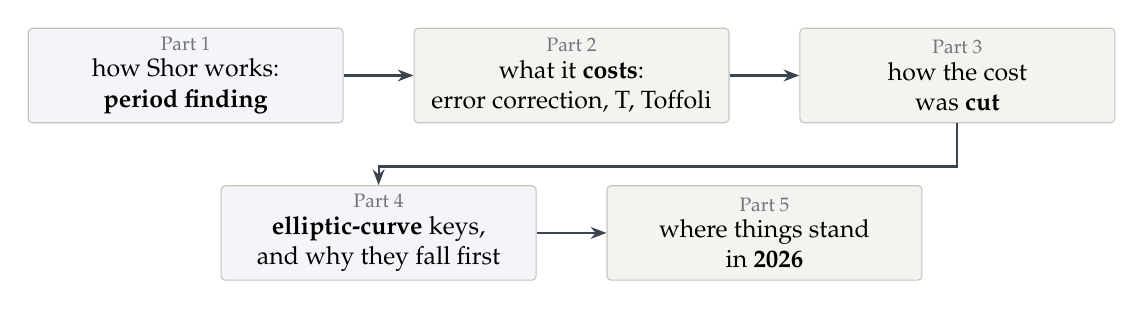
\begin{tikzpicture}[
      stage/.style={draw=rulegrey,fill=greybox,rounded corners=1.5pt,align=center,
        minimum width=40mm,minimum height=12mm,font=\small,inner sep=2pt},
      quantum/.style={stage,fill=lavender},
      arr/.style={-{Stealth[length=2mm]},color=body,thick}]
    \node[quantum] (a) at (0,0)     {\actlab{Part 1}how Shor works:\\\textbf{period finding}};
    \node[stage]   (b) at (4.9,0)   {\actlab{Part 2}what it \textbf{costs}:\\error correction, T, Toffoli};
    \node[stage]   (c) at (9.8,0)   {\actlab{Part 3}how the cost\\was \textbf{cut}};
    \node[quantum] (d) at (2.45,-2) {\actlab{Part 4}\textbf{elliptic-curve} keys,\\and why they fall first};
    \node[stage]   (e) at (7.35,-2) {\actlab{Part 5}where things stand\\in \textbf{2026}};
    \draw[arr] (a) -- (b); \draw[arr] (b) -- (c);
    \draw[arr] (c.south) |- ++(0,-0.55) -| (d.north);
    \draw[arr] (d) -- (e);
  \end{tikzpicture}\par
  \vskip4mm
  \raggedright\small
  Each part answers one question, and each step uses only what came before it. Two background slides fill in what we need along the way: qubits and phases (now), error correction (Part 2).
  \begin{takeaway}Almost all of Shor's cost is reversible arithmetic: that is what we build, run and count.\end{takeaway}
\end{frame}}

% ======================================================================
\act{Part 1 --- How Shor works}

{\setbeamertemplate{footline}{\hfill{\scriptsize\color{ink}N2}\hspace*{5mm}\vskip3mm}
\begin{frame}[noframenumbering]{Background: qubits, gates and phases}
  \begin{columns}[T,onlytextwidth]
    \begin{column}{0.485\textwidth}
      \begin{panel}[equal height group=bgq]
        \blocktitle{States}
        \small
        A qubit is $\alpha|0\rangle+\beta|1\rangle$; measuring gives 0 with probability $|\alpha|^2$, 1 with $|\beta|^2$.\par\vskip1mm
        $n$ qubits hold $2^n$ amplitudes, one per integer: $\sum_x\alpha_x|x\rangle$. Registers combine by $\otimes$: $|a\rangle\otimes|b\rangle=|a\rangle|b\rangle$.\par\vskip1mm
        \textbf{Phases.} A global phase $e^{i\theta}|\psi\rangle$ changes nothing. A \textbf{relative} phase, $\alpha|0\rangle+e^{i\theta}\beta|1\rangle$, is real: interference can read it.
      \end{panel}
    \end{column}
    \begin{column}{0.485\textwidth}
      \begin{panel}[equal height group=bgq]
        \blocktitle{Gates}
        \small
        $H$: $|0\rangle\mapsto\tfrac{|0\rangle+|1\rangle}{\sqrt2}$, $|1\rangle\mapsto\tfrac{|0\rangle-|1\rangle}{\sqrt2}$. \ $X$: NOT. \ $P(\theta)$: $|1\rangle\mapsto e^{i\theta}|1\rangle$.\par\vskip1mm
        CNOT: $|a,b\rangle\mapsto|a,b\oplus a\rangle$. Controlled-$U$: apply $U$ only where the control is 1.\par\vskip1mm
        QFT: $|x\rangle\mapsto\frac{1}{\sqrt Q}\sum_y e^{2\pi i\,xy/Q}|y\rangle$ writes $x$ as a \textbf{phase ramp}; QFT$^\dagger$ reads a ramp back as an integer.
      \end{panel}
    \end{column}
  \end{columns}
  \vskip1mm
  \begin{takeaway}Gates act on every branch of a superposition at once; the answer comes from interference, phases arranged so wrong answers cancel.\end{takeaway}
\end{frame}}

\setcounter{framenumber}{2}
\begin{frame}{Act I --- factoring reduces to finding a period}
  \begin{difficulty}{1}To factor $N$, pick $a$ with $\gcd(a,N)=1$ and find its \textbf{order} \per{$r$}: the smallest $r>0$ with $a^r\equiv1 \pmod N$.\end{difficulty}
  \centering
  \renewcommand{\arraystretch}{1.2}
  \begin{tabular}{c|ccccccc}
    $x$ & 0 & 1 & 2 & 3 & 4 & 5 & $\cdots$\\ \hline
    $7^x \bmod 15$ & 1 & 7 & 4 & 13 & 1 & 7 & $\cdots$
  \end{tabular}
  \qquad $\Rightarrow\ \per{r=4}$
  \vskip2mm
  \raggedright
  Why the period factors $N$: if $r$ is even, $N$ divides
  \[ a^r-1=(a^{r/2}-1)(a^{r/2}+1), \]
  and unless $a^{r/2}\equiv-1$ each factor shares a divisor with $N$: \ $\gcd(48,15)=3$, \ $\gcd(50,15)=5$.
  \begin{takeaway}The period is a property of the whole sequence, not of any one value. Only the period needs a quantum computer; the rest is Euclid.\end{takeaway}
\end{frame}

\setcounter{framenumber}{3}
\begin{frame}{Phase estimation: the circuit}
  \centering
  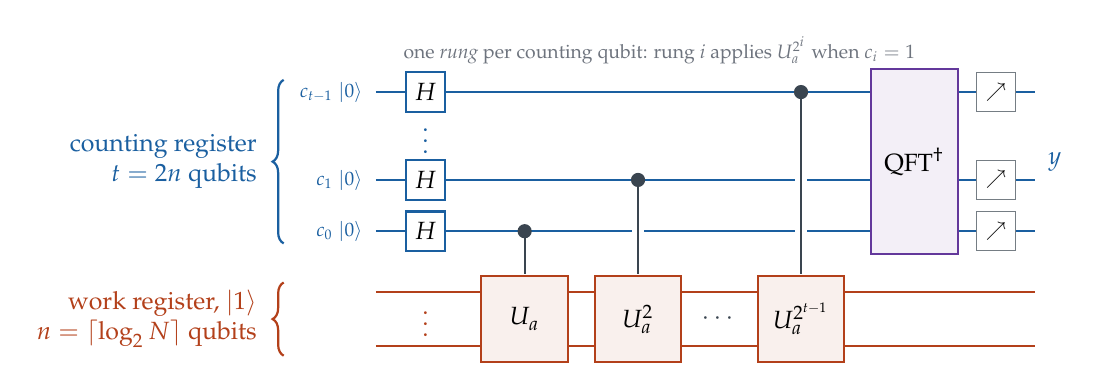
\begin{tikzpicture}[x=9mm,y=6.2mm]
    % counting register: c_0 at the bottom, c_{t-1} at the top; the gap row carries the dots
    \foreach \y/\q in {5.45/{t-1},3.65/1,2.6/0} {
      \node[font=\scriptsize,color=cblue,anchor=east] at (-0.05,\y) {$c_{\q}\;|0\rangle$};
      \draw[cwire] (0,\y) -- (9.3,\y);
      \node[hop] at (0.7,\y) {$H$};}
    \node[font=\small,color=cblue] at (0.7,4.62) {$\vdots$};
    % work register: n qubits holding the integer 1
    \foreach \y in {1.35,0.25} \draw[twire] (0,\y) -- (9.3,\y);
    \node[font=\small,color=cverm] at (0.7,0.86) {$\vdots$};
    % braces
    \draw[decorate,decoration={brace,amplitude=4pt},thick,color=cblue] (-1.3,2.35) -- (-1.3,5.7)
      node[midway,left=6pt,font=\small,align=right,color=cblue] {counting register\\$t=2n$ qubits};
    \draw[decorate,decoration={brace,amplitude=4pt},thick,color=cverm] (-1.3,0.05) -- (-1.3,1.55)
      node[midway,left=6pt,font=\small,align=right,color=cverm] {work register, $|1\rangle$\\$n=\lceil\log_2N\rceil$ qubits};
    % rungs: each control line hops over the wires it crosses
    \foreach \x/\y/\p in {2.1/2.6/{}, 3.7/3.65/{2}, 6.0/5.45/{2^{t-1}}} {
      \draw[white,line width=4pt] (\x,\y-0.28) -- (\x,1.75);
      \draw[thick,color=body] (\x,\y) -- (\x,1.72);
      \node[dot] at (\x,\y) {};
      \node[op,minimum width=11mm,minimum height=11mm] at (\x,0.8) {$U_a^{\p}$};}
    \node[font=\small,color=body] at (4.85,0.8) {$\cdots$};
    % inverse QFT and readout
    \node[qop,minimum height=23.5mm,minimum width=11mm] at (7.6,4.025) {$\mathrm{QFT}^\dagger$};
    \foreach \y in {5.45,3.65,2.6} \node[meter] at (8.75,\y) {$\nearrow$};
    \node[font=\small,color=cblue,anchor=west] at (9.35,4.025) {$y$};
    \node[note] at (4.0,6.3) {one \emph{rung} per counting qubit: rung $i$ applies $U_a^{2^i}$ when $c_i=1$};
  \end{tikzpicture}
  \vskip0.5mm
  \[
    U_{\text{Shor}}=\big(\per{\mathrm{QFT}^\dagger}\otimes I\big)\;
    \text{C-}\tgt{U_a^{2^{t-1}}}\cdots\,\text{C-}\tgt{U_a^{2}}\;\text{C-}\tgt{U_a}\;
    \big(\cnt{H^{\otimes t}}\otimes I\big)\quad\text{applied to}\quad \cnt{|0\rangle^{\otimes t}}\,\tgt{|1\rangle}
  \]
  \vskip-1mm
  {\small where $\text{C-}U=|0\rangle\langle0|\otimes I+|1\rangle\langle1|\otimes U$, and $U_a^{2^i}=U_{a^{2^i}\bmod N}$ is computed classically.}
\end{frame}

{\setbeamertemplate{footline}{\hfill{\scriptsize\color{ink}N3}\hspace*{5mm}\vskip3mm}
\begin{frame}[noframenumbering]{Phase kickback: how the control learns the phase}
  \small
  If $|\psi\rangle$ is an eigenvector, $U|\psi\rangle=e^{2\pi i\varphi}|\psi\rangle$, a controlled-$U$ does this:
  \[ \text{C-}U\,(\alpha|0\rangle+\beta|1\rangle)|\psi\rangle
     \;\underset{\text{linearity}}{=}\;\alpha|0\rangle|\psi\rangle+\beta|1\rangle\,e^{2\pi i\varphi}|\psi\rangle
     \;\underset{\text{bilinearity}}{=}\;\big(\alpha|0\rangle+e^{2\pi i\varphi}\beta|1\rangle\big)|\psi\rangle . \]
  \begin{columns}[T,onlytextwidth]
    \begin{column}{0.485\textwidth}
      \begin{panel}[equal height group=kb]
        \blocktitle{Why}
        Linearity: only the $|1\rangle$ branch gets the phase. Bilinearity: a number on a product belongs to neither factor, $(\lambda a)\otimes b=a\otimes(\lambda b)$. Global on the target, so invisible; \textbf{relative} on the control, so readable.
      \end{panel}
    \end{column}
    \begin{column}{0.485\textwidth}
      \begin{panel}[equal height group=kb]
        \blocktitle{Check on two qubits}
        CNOT on $|+\rangle|-\rangle$ gives $|-\rangle|-\rangle$: the ``target'' is unchanged and the ``control'' flipped, because $X|-\rangle=-|-\rangle$. The phase belongs to the pair.
      \end{panel}
    \end{column}
  \end{columns}
  \vskip1mm
  \begin{takeaway}In Shor, rung $j$ kicks $e^{2\pi i\,2^j s/r}$ onto counting qubit $j$: together, the phase ramp $\sum_x e^{2\pi i\,x s/r}|x\rangle$.\end{takeaway}
\end{frame}}

\setcounter{framenumber}{4}
\begin{frame}{Why the measurement reveals $s/r$}
  \setlength{\abovedisplayskip}{2pt}\setlength{\belowdisplayskip}{2pt}\setlength{\parskip}{2pt}
  \begin{enumerate}
    \setlength{\itemsep}{2.5mm}
    \item \textbf{Eigenvectors.} \ $U_a|u_s\rangle=e^{2\pi i\,\per{\varphi}}|u_s\rangle$, \ $\per{\varphi=s/r}$; \ the input is $\tgt{|1\rangle}=\frac{1}{\sqrt r}\sum_{s}|u_s\rangle$.
    \item \textbf{Kickback.} Rung $j$ leaves $|u_s\rangle$ alone and turns its control by $2^j\per{\varphi}$. The counting register ($Q=2^t$) becomes a product:
      \[ \bigotimes_{j}\frac{|0\rangle+e^{2\pi i\,2^j\per{\varphi}}|1\rangle}{\sqrt2}
         =\frac{1}{\sqrt Q}\sum_{x=0}^{Q-1}e^{2\pi i\,\per{\varphi}\,\cnt{x}}\,\cnt{|x\rangle}=:|\Phi_{\per{\varphi}}\rangle \]
      {\small since branch $\cnt{x}$ collects the turns of its 1-bits, $\prod_j e^{2\pi i\,2^j\per{\varphi}\,x_j}=e^{2\pi i\,\per{\varphi}\,\cnt{x}}$: a \emph{phase ramp} of slope $\per{\varphi}$.}
    \item \textbf{Readout.} With $\langle y|\,\mathrm{QFT}^\dagger|x\rangle=e^{-2\pi i\,xy/Q}/\sqrt Q$:
      \[ \langle y|\,\mathrm{QFT}^\dagger|\Phi_{\per{\varphi}}\rangle
         =\frac1Q\sum_{x}e^{-2\pi i\,xy/Q}\,e^{2\pi i\,\per{\varphi}x}
         =\frac1Q\sum_{x=0}^{Q-1}e^{2\pi i\,(\per{\varphi}-y/Q)\,x}
         =\begin{cases}\approx1, & y\approx Q\per{\varphi}\\[-1pt] \approx0, & \text{otherwise}\end{cases} \]
      {\small Each $|u_s\rangle$ carries its own ramp; they do not interfere: $y\approx Q\,\per{s/r}$, $s$ uniformly random.}
  \end{enumerate}
\end{frame}

\setcounter{framenumber}{5}
\begin{frame}{$\mathrm{QFT}^\dagger$ in action: a ramp becomes an integer}
  $t=3$, $\per{s/r=1/4}$: the phase $e^{2\pi i\,x/4}=i^{\,x}$ turns a quarter turn per step:
  \vskip-1mm
  \[
    \frac{1}{\sqrt8}\sum_{x=0}^{7}e^{2\pi i\,x/4}\,|x\rangle
    =\frac{|0\rangle+i|1\rangle-|2\rangle-i|3\rangle+|4\rangle+\cdots}{\sqrt8}
    =\mathrm{QFT}\,|2\rangle
    \;\xrightarrow{\;\mathrm{QFT}^\dagger\;}\;\cnt{|2\rangle}
  \]
  \par\centering\fig[width=0.88\textwidth]{qft_readout_exact.pdf}
  \begin{takeaway}Every shot gives $y=2$: $s/r=2/8=1/4$, the ramp's slope read as an integer.\end{takeaway}
\end{frame}

\setcounter{framenumber}{32}
\begin{frame}{$N=15$: four sharp peaks}
  \begin{columns}[c]
    \begin{column}{0.5\textwidth}
      \centering\fig[width=\textwidth]{n15_hist.pdf}
    \end{column}
    \begin{column}{0.46\textwidth}
      \blocktitle{The exact distribution}
      The target takes $r$ values, one per residue $x_0=x \bmod r$:
      \[ P(y)=\frac{1}{4^{t}}\sum_{x_0<r}\Big|\sum_{m} e^{-2\pi i\,m r y/2^t}\Big|^2 \]
      Aer's exact probabilities equal it.
    \end{column}
  \end{columns}
  \vskip1mm
  {\small \textbf{Samples vs exact:} the total variation distance $\tfrac12\sum_y|\hat p(y)-p(y)|$ is $0.006$. A perfect sampler exceeds $0.032$ only 0.01\% of the time at 4096 shots --- the \emph{shot-noise bound}.}
\end{frame}

% ======================================================================
\act{Part 2 --- What it costs}

{\setbeamertemplate{footline}{\hfill{\scriptsize\color{ink}N4}\hspace*{5mm}\vskip3mm}
\begin{frame}[noframenumbering]{Background: error correction in one slide}
  \begin{columns}[T,onlytextwidth]
    \begin{column}{0.6\textwidth}
      \small
      \textbf{Why.} Physical qubits fail about once per $10^3$ gates; Shor needs $10^8$--$10^{10}$ Toffolis.\par\vskip0.8mm
      \textbf{Logical qubits.} Store one protected qubit in many physical ones, e.g.\ $\alpha|000\rangle+\beta|111\rangle$. \textbf{Parity checks} (``are qubits 1 and 2 equal?'') locate an error without reading $\alpha,\beta$; a decoder fixes it.\par\vskip0.8mm
      \textbf{Distance $d$, threshold.} Below about $1\%$ physical error, the logical error falls exponentially with $d$: $d\approx27$ at $p=10^{-3}$.\par\vskip0.8mm
      \textbf{Cheap gates.} \emph{Transversal} gates act qubit by qubit, so one fault stays one error. On the surface code the Clifford gates ($H$, $S$, CNOT) are cheap; $T$ is not.
    \end{column}
    \begin{column}{0.36\textwidth}
      \centering
      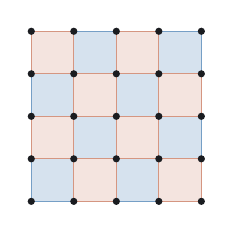
\begin{tikzpicture}[x=5.4mm,y=5.4mm]
        \foreach \i/\j in {0/0,0/2,1/1,1/3,2/0,2/2,3/1,3/3} \fill[cblue!18,draw=cblue!60] (\i,\j) rectangle ++(1,1);
        \foreach \i/\j in {0/1,0/3,1/0,1/2,2/1,2/3,3/0,3/2} \fill[cverm!14,draw=cverm!55] (\i,\j) rectangle ++(1,1);
        \foreach \i in {0,...,4} \foreach \j in {0,...,4} \fill[ink] (\i,\j) circle (1.3pt);
      \end{tikzpicture}\par
      \vskip1mm
      {\scriptsize Surface code, $d=5$: dots are data qubits, squares are checks of $Z$ (blue) or $X$ (red) type on 4 neighbours. About $2d^2$ physical qubits per logical one: ${\approx}1\,500$ at $d=27$.}
    \end{column}
  \end{columns}
  \begin{takeaway}Error correction makes Clifford gates cheap and leaves one gate expensive: $T$.\end{takeaway}
\end{frame}}

{\setbeamertemplate{footline}{\hfill{\scriptsize\color{ink}N5}\hspace*{5mm}\vskip3mm}
\begin{frame}[noframenumbering]{The surface code: parity checks, errors and the decoder}
  \begin{columns}[T,onlytextwidth]
    \begin{column}{0.56\textwidth}
      \small
      \textbf{Measure parities, never the data.} Every cycle (about $1\,\mu$s) each square measures the parity of its four corners: \cnt{$Z$-squares} catch bit flips, \tgt{$X$-squares} phase flips. No check reveals the stored state.\par\vskip0.8mm
      \textbf{Find the errors.} An error flips the squares next to it; a chain of errors flips only its two ends. A classical \emph{decoder} pairs the flipped squares and infers the correction.\par\vskip0.8mm
      \textbf{Where the qubit lives.} The logical operator is a string across the whole patch (\per{purple}). Corrupting it takes $d$ errors in a line: the distance.
    \end{column}
    \begin{column}{0.4\textwidth}
      \centering
      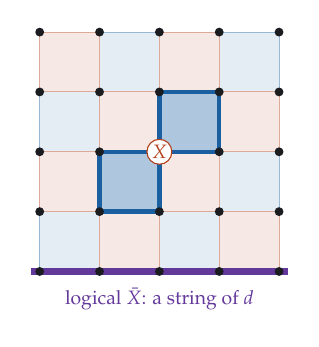
\begin{tikzpicture}[x=7.6mm,y=7.6mm]
        \foreach \i/\j in {0/0,0/2,1/1,1/3,2/0,2/2,3/1,3/3} \fill[cblue!12,draw=cblue!45] (\i,\j) rectangle ++(1,1);
        \foreach \i/\j in {0/1,0/3,1/0,1/2,2/1,2/3,3/0,3/2} \fill[cverm!12,draw=cverm!45] (\i,\j) rectangle ++(1,1);
        \foreach \i/\j in {1/1,2/2} \draw[cblue,line width=1.6pt,fill=cblue!35] (\i,\j) rectangle ++(1,1);
        \draw[cpurple,line width=2.2pt] (-0.15,0) -- (4.15,0);
        \foreach \i in {0,...,4} \foreach \j in {0,...,4} \fill[ink] (\i,\j) circle (1.6pt);
        \node[draw=cverm,fill=white,circle,inner sep=0.6pt,font=\scriptsize\bfseries,text=cverm] at (2,2) {$X$};
        \node[font=\scriptsize,color=cpurple,anchor=north] at (2,-0.12) {logical $\bar X$: a string of $d$};
      \end{tikzpicture}\par
      \vskip0.5mm
      {\scriptsize $d=5$. One bit flip (centre) lights the two $Z$-squares beside it.}
    \end{column}
  \end{columns}
  \vskip1mm
  \begin{takeaway}Below threshold ($p_{\mathrm{th}}\approx1\%$), $P_L\approx(p/p_{\mathrm{th}})^{(d+1)/2}$: at $p=10^{-3}$, each $d\to d+2$ divides it by about 10.\end{takeaway}
\end{frame}}

{\setbeamertemplate{footline}{\hfill{\scriptsize\color{ink}N8}\hspace*{5mm}\vskip3mm}
\begin{frame}[noframenumbering]{The surface code as parity checks, at $d=3$}
  \begin{columns}[T,onlytextwidth]
    \begin{column}{0.36\textwidth}
      \centering
      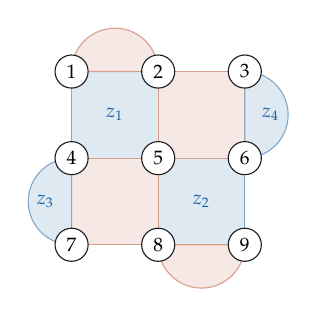
\begin{tikzpicture}[x=11mm,y=11mm]
        \fill[cblue!14,draw=cblue!55] (0,-1) rectangle (1,0);
        \fill[cblue!14,draw=cblue!55] (1,-2) rectangle (2,-1);
        \fill[cverm!12,draw=cverm!50] (1,-1) rectangle (2,0);
        \fill[cverm!12,draw=cverm!50] (0,-2) rectangle (1,-1);
        \fill[cverm!12,draw=cverm!50] (0,0) arc (180:0:0.5) -- cycle;
        \fill[cverm!12,draw=cverm!50] (1,-2) arc (180:360:0.5) -- cycle;
        \fill[cblue!14,draw=cblue!55] (0,-1) arc (90:270:0.5) -- cycle;
        \fill[cblue!14,draw=cblue!55] (2,0) arc (90:-90:0.5) -- cycle;
        \node[font=\scriptsize,color=cblue] at (0.5,-0.5) {$z_1$};
        \node[font=\scriptsize,color=cblue] at (1.5,-1.5) {$z_2$};
        \node[font=\scriptsize,color=cblue] at (-0.3,-1.5) {$z_3$};
        \node[font=\scriptsize,color=cblue] at (2.3,-0.5) {$z_4$};
        \foreach \c/\r/\q in {0/0/1,1/0/2,2/0/3,0/1/4,1/1/5,2/1/6,0/2/7,1/2/8,2/2/9}
          \node[circle,fill=white,draw=ink,inner sep=0.8pt,minimum size=4.2mm,font=\scriptsize] at (\c,-\r) {\q};
      \end{tikzpicture}\par
      \vskip1mm
      {\scriptsize 9 data qubits; \tgt{red} $X$-checks catch $Z$ errors, \cnt{blue} $Z$-checks catch $X$ errors.}
    \end{column}
    \begin{column}{0.6\textwidth}
      \small\setlength{\abovedisplayskip}{2pt}\setlength{\belowdisplayskip}{2pt}%
      $Z$-checks as a parity-check matrix $H_Z$; an $X$ error $e$ gives $s=H_Ze$. Each check asks: \emph{did an odd number of $X$ errors hit my qubits?}
      \[ {\scriptsize\setlength{\arraycolsep}{2.6pt}\begin{array}{r|ccccccccc}
           & 1&2&3&4&5&6&7&8&9\\ \hline
         z_1 & 1&1&0&1&1&0&0&0&0\\
         z_2 & 0&0&0&0&1&1&0&1&1\\
         z_3 & 0&0&0&1&0&0&1&0&0\\
         z_4 & 0&0&1&0&0&1&0&0&0 \end{array}} \]
      \textbf{Narrowing down.} $X_5$ lights $z_1,z_2$: only qubit 5 is in both; $X_7$ lights $z_3$ alone.\par\vskip0.5mm
      \textbf{Degenerate.} $X_1$, $X_2$ give one syndrome, but $X_1X_2$ is a check: either fix works.
    \end{column}
  \end{columns}
  \begin{takeaway}$[[9,1,3]]$: 8 checks, 1 logical qubit ($\bar X=X_1X_4X_7$, $\bar Z=Z_1Z_2Z_3$), distance 3: every single error is fixed.\end{takeaway}
\end{frame}}

{\setbeamertemplate{footline}{\hfill{\scriptsize\color{ink}N7}\hspace*{5mm}\vskip3mm}
\begin{frame}[noframenumbering]{How error correction runs: measure, decode, keep going}
  \begin{columns}[T,onlytextwidth]
    \begin{column}{0.485\textwidth}
      \begin{panel}[equal height group=ecr]
        \blocktitle{On the chip (quantum)}
        \small
        Every ${\approx}1\,\mu$s every check is measured, in parallel with the computation.\par\vskip1mm
        A check reads a parity, never the data: the computation \textbf{never stops}.\par\vskip1mm
        Logical gates are themselves check measurements (lattice surgery).
      \end{panel}
    \end{column}
    \begin{column}{0.485\textwidth}
      \begin{panel}[equal height group=ecr]
        \blocktitle{In the decoder (classical)}
        \small
        Watches for checks whose result \textbf{changes}: errors show in space, faulty measurements in time.\par\vskip1mm
        Pairs the changes into the most likely errors.\par\vskip1mm
        Records the correction in software (the \emph{Pauli frame}); no gate is applied.
      \end{panel}
    \end{column}
  \end{columns}
  \vskip1mm
  \begin{takeaway}Never stop to correct. Wait only at $T$ gates, whose correction needs the decoder's answer: the ${\approx}10\,\mu$s reaction time.\end{takeaway}
\end{frame}}

{\setbeamertemplate{footline}{\hfill{\scriptsize\color{ink}N9}\hspace*{5mm}\vskip3mm}
\begin{frame}[noframenumbering]{Codes, their parameters, and the bounds}
  \begin{columns}[T,onlytextwidth]
    \begin{column}{0.47\textwidth}
      \small
      $[[n,k,d]]$: $n$ physical qubits store $k$ logical ones; $d$ is the fewest single-qubit errors that change the data unseen. It corrects $\lfloor(d-1)/2\rfloor$ errors.\par\vskip1mm
      \centering\footnotesize
      \renewcommand{\arraystretch}{1.12}
      \begin{tabular}{@{}ll@{}}
        \toprule
        code & $[[n,k,d]]$ \\
        \midrule
        five-qubit (smallest) & $[[5,1,3]]$ \\
        Steane & $[[7,1,3]]$ \\
        surface, rotated & $[[d^2,1,d]]$ \\
        IBM gross (qLDPC) & $[[144,12,12]]$ \\
        good qLDPC (2021) & $[[n,\Theta(n),\Theta(n)]]$ \\
        \bottomrule
      \end{tabular}
    \end{column}
    \begin{column}{0.49\textwidth}
      \begin{panel}
        \blocktitle{How well can a code do?}
        \small
        \textbf{Singleton:} $n-k\ge2(d-1)$.\par\vskip0.6mm
        \textbf{Hamming:} $2^{n-k}\ge\sum_{j\le t}\binom{n}{j}3^j$; $[[5,1,3]]$ meets it ($16=1+15$).\par\vskip0.6mm
        \textbf{Local checks on a flat chip:} $k\,d^2=O(n)$ (Bravyi--Poulin--Terhal). The surface code meets it.\par\vskip0.6mm
        \textbf{Cheap gates:} never universal (Eastin--Knill), so $T$ needs magic states.
      \end{panel}
    \end{column}
  \end{columns}
  \vskip1mm
  \begin{takeaway}On a flat chip with local checks, about $d^2$ qubits per logical qubit is the best possible; doing better needs long-range links (qLDPC).\end{takeaway}
\end{frame}}

{\setbeamertemplate{footline}{\hfill{\scriptsize\color{ink}N10}\hspace*{5mm}\vskip3mm}
\begin{frame}[noframenumbering]{Which codes can exist: the bounds}
  \begin{columns}[T,onlytextwidth]
    \begin{column}{0.56\textwidth}
      \centering
      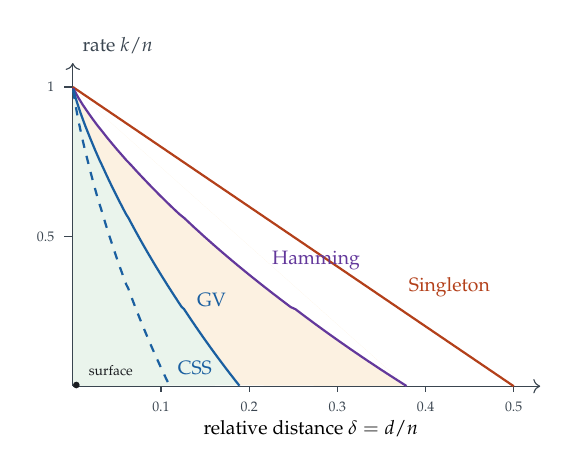
\begin{tikzpicture}[x=112mm,y=38mm]
        \fill[okfill] (0.0005,1) plot[domain=0.0005:0.1893,samples=60] (\x,{1-\x*ln(3)/ln(2)+\x*ln(\x)/ln(2)+(1-\x)*ln(1-\x)/ln(2)}) -- (0,0) -- cycle;
        \fill[lkfill] (0.0005,1) plot[domain=0.0005:0.1893,samples=60] (\x,{1-\x*ln(3)/ln(2)+\x*ln(\x)/ln(2)+(1-\x)*ln(1-\x)/ln(2)}) -- (0.3786,0) plot[domain=0.3786:0.0005,samples=60] (\x,{1-(\x/2)*ln(3)/ln(2)+(\x/2)*ln(\x/2)/ln(2)+(1-\x/2)*ln(1-\x/2)/ln(2)}) -- cycle;
        \draw[->,color=body] (0,0) -- (0.53,0); \node[font=\scriptsize] at (0.27,-0.14) {relative distance $\delta=d/n$};
        \draw[->,color=body] (0,0) -- (0,1.08) node[above right,font=\scriptsize] {rate $k/n$};
        \foreach \t in {0.1,0.2,0.3,0.4,0.5} \draw[color=body] (\t,0) -- (\t,-0.02) node[below,font=\tiny] {\t};
        \foreach \t in {0.5,1} \draw[color=body] (0,\t) -- (-0.01,\t) node[left,font=\tiny] {\t};
        \draw[cverm,thick] (0,1) -- (0.5,0);
        \draw[cpurple,thick,domain=0.0005:0.3786,samples=70] plot (\x,{1-(\x/2)*ln(3)/ln(2)+(\x/2)*ln(\x/2)/ln(2)+(1-\x/2)*ln(1-\x/2)/ln(2)});
        \draw[cblue,thick,domain=0.0005:0.1893,samples=70] plot (\x,{1-\x*ln(3)/ln(2)+\x*ln(\x)/ln(2)+(1-\x)*ln(1-\x)/ln(2)});
        \draw[cblue,thick,dashed,domain=0.0005:0.1100,samples=50] plot (\x,{1+2*\x*ln(\x)/ln(2)+2*(1-\x)*ln(1-\x)/ln(2)});
        \node[font=\scriptsize,color=cverm,anchor=west] at (0.37,0.33) {Singleton};
        \node[font=\scriptsize,color=cpurple,anchor=west] at (0.215,0.42) {Hamming};
        \node[font=\scriptsize,color=cblue,anchor=west] at (0.13,0.29) {GV};
        \node[font=\scriptsize,color=cblue,anchor=west] at (0.108,0.06) {CSS};
        \fill[ink] (0.004,0.004) circle (1.2pt) node[above right,font=\tiny,xshift=1pt,yshift=0pt] {surface};
      \end{tikzpicture}
    \end{column}
    \begin{column}{0.42\textwidth}
      \footnotesize
      Large codes, rate $k/n$, relative distance $\delta=d/n$:\par\vskip1mm
      \tgt{\textbf{Singleton:}} $k/n\le1-2\delta$.\par\vskip0.8mm
      \per{\textbf{Hamming:}} $k/n\le1-\tfrac{\delta}{2}\log_23-H_2(\tfrac{\delta}{2})$; tighter than Singleton.\par\vskip0.8mm
      \cnt{\textbf{Gilbert--Varshamov:}} codes \emph{exist} with $k/n\ge1-\delta\log_23-H_2(\delta)$; CSS codes with $1-2H_2(\delta)$ (dashed).\par\vskip0.8mm
      Surface code: at the origin. Good qLDPC codes: constant $k/n$ and $d/n$, with long-range links.
    \end{column}
  \end{columns}
  \vskip1mm
  \begin{takeaway}Green: codes exist. Peach: open. Above the Hamming curve: impossible for large codes.\end{takeaway}
\end{frame}}

{\setbeamertemplate{footline}{\hfill{\scriptsize\color{ink}N6}\hspace*{5mm}\vskip3mm}
\begin{frame}[noframenumbering]{From one patch to a computer}
  \begin{columns}[T,onlytextwidth]
    \begin{column}{0.485\textwidth}
      \begin{panel}[equal height group=sc2]
        \blocktitle{How big a patch}
        \small
        A Shor run has about $10^3$ logical qubits for $10^9$--$10^{10}$ cycles, so it needs $P_L\approx10^{-15}$ per qubit per cycle.\par\vskip1mm
        With a factor 10 per step: $d\approx27$, so $2d^2\approx1\,500$ physical qubits per logical one, plus routing and factories.\par\vskip1mm
        Measured: on Google's Willow (2024) the logical error halved at each step $d=3\to5\to7$.
      \end{panel}
    \end{column}
    \begin{column}{0.485\textwidth}
      \begin{panel}[equal height group=sc2]
        \blocktitle{How it computes}
        \small
        $X$, $Z$: free, tracked in software.\par\vskip1mm
        CNOT: \textbf{lattice surgery}. Merge two patches along an edge, measure their joint checks for about $d$ cycles, split.\par\vskip1mm
        $H$, $S$: cheap, by similar tricks.\par\vskip1mm
        $T$: impossible this way (Eastin--Knill): a \textbf{magic state} from a factory, consumed by lattice surgery.
      \end{panel}
    \end{column}
  \end{columns}
  \vskip1mm
  \begin{takeaway}A machine is a floor of patches: memory, routing and magic-state factories. The Toffoli count sets the runtime.\end{takeaway}
\end{frame}}

\setcounter{framenumber}{10}
\begin{frame}{Why the $T$ gate is the expensive one}
  \begin{columns}[T]
    \begin{column}{0.47\textwidth}
      \begin{greyblock}
        \blocktitle{Transversal gates}
        A \emph{logical} qubit is spread over many physical qubits. The safest logical gate is \textbf{transversal}: the same gate on every physical qubit, so a fault cannot spread. On the surface code CNOT is transversal and $H$, $S$ nearly so: Cliffords are cheap.
      \end{greyblock}
    \end{column}
    \begin{column}{0.47\textwidth}
      \begin{greyblock}
        \blocktitle{Eastin--Knill (2009)}
        No code has a transversal gate set that is \emph{universal}. A code that ignores small local errors cannot let small local operations move its logical state. Some gate must be done another way: $T$.
      \end{greyblock}
    \end{column}
  \end{columns}
  \begin{takeaway}Eastin--Knill makes the gate set finite; Solovay--Kitaev makes that affordable; magic states are the price of $T$.\end{takeaway}
\end{frame}

\setcounter{framenumber}{11}
\begin{frame}{Magic states: $T$ by teleportation}
  \centering
  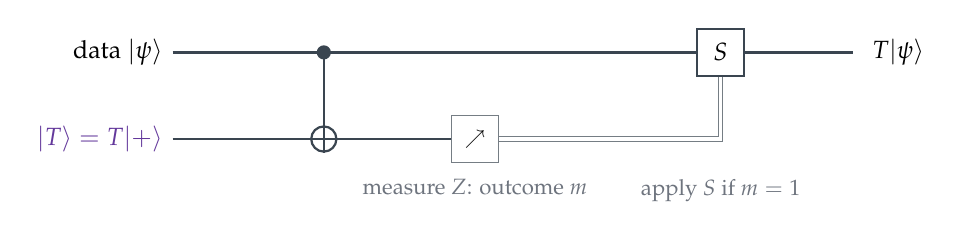
\begin{tikzpicture}[x=12mm,y=11mm]
    \node[lab] at (0,1) {data $|\psi\rangle$}; \draw[wire] (0,1) -- (7.2,1);
    \node[lab,color=cpurple] at (0,0) {$|T\rangle=T|{+}\rangle$}; \draw[wire] (0,0) -- (3.2,0);
    \draw[clw] (3.43,0) -- (5.8,0) -- (5.8,0.73);
    \draw[thick,color=body] (1.6,1) -- (1.6,0); \node[dot] at (1.6,1) {}; \oplusat{1.6}{0}
    \node[meter,minimum size=6mm] at (3.2,0) {$\nearrow$};
    \node[draw=body,fill=white,thick,minimum size=6mm,font=\small,inner sep=1pt] at (5.8,1) {$S$};
    \node[font=\small,anchor=west] at (7.3,1) {$T|\psi\rangle$};
    \node[note,anchor=north,font=\footnotesize] at (3.2,-0.35) {measure $Z$: outcome $m$};
    \node[note,anchor=north,font=\footnotesize] at (5.8,-0.35) {apply $S$ if $m=1$};
  \end{tikzpicture}
  \vskip3mm
  \begin{columns}[T]
    \begin{column}{0.47\textwidth}
      \blocktitle{Why it works}
      After the CNOT, $m=0$ leaves $T|\psi\rangle$ and $m=1$ leaves $T^\dagger|\psi\rangle$; $S\,T^\dagger=T$. CNOT, measurement and $S$ are all Clifford: the gate costs \textbf{one fresh $|T\rangle$}.
    \end{column}
    \begin{column}{0.47\textwidth}
      \blocktitle{Factories}
      Regions of the chip that produce $|T\rangle$. \emph{Distillation} (2005): 15 noisy copies $\to$ 1 with error $\approx35\varepsilon^3$. \emph{Cultivation} (2024): grow one copy inside a small code, checking as it grows; $\approx10\times$ cheaper.
    \end{column}
  \end{columns}
\end{frame}

\setcounter{framenumber}{12}
\begin{frame}{The Toffoli: a reversible AND}
  \[ \mathrm{Toffoli}\;|a,\,b,\,c\rangle = |a,\,b,\,c\oplus ab\rangle \]
  \vskip1mm
  \begin{columns}[T]
    \begin{column}{0.47\textwidth}
      \blocktitle{Reversible: it permutes basis states}
      It swaps $|110\rangle\leftrightarrow|111\rangle$ and fixes the other six. A permutation matrix is unitary; its inverse is the reverse permutation, here the Toffoli itself:
      \[ c\oplus ab\oplus ab=c . \]
    \end{column}
    \begin{column}{0.47\textwidth}
      \blocktitle{What it costs}
      In Clifford+T, a Toffoli is \textbf{7 T gates}. A classical function is therefore priced exactly by its Toffoli count.
    \end{column}
  \end{columns}
  \begin{takeaway}Reversible arithmetic = Toffolis + CNOTs. Its T cost is exact: $7\times$ the number of Toffolis.\end{takeaway}
\end{frame}

{\setbeamertemplate{footline}{\hfill{\scriptsize\color{ink}N11}\hspace*{5mm}\vskip3mm}
\begin{frame}[noframenumbering]{Irreversible functions as unitaries: the three tricks}
  \begin{columns}[T,onlytextwidth]
    \begin{column}{0.315\textwidth}
      \begin{panel}[equal height group=rv]
        \blocktitle{1. Keep the input}
        \footnotesize\setlength{\abovedisplayskip}{2pt}\setlength{\belowdisplayskip}{2pt}%
        Any $f$, even many-to-one:
        \[ U_f|x,y\rangle=|x,\,y\oplus f(x)\rangle \]
        A permutation of basis states: unitary, its own inverse. Built from NOT, CNOT (XOR) and Toffoli (AND).
      \end{panel}
    \end{column}
    \begin{column}{0.315\textwidth}
      \begin{panel}[equal height group=rv]
        \blocktitle{2. Clean the scratch}
        \footnotesize\setlength{\abovedisplayskip}{2pt}\setlength{\belowdisplayskip}{2pt}%
        Gates leave garbage $g(x)$ (Bennett):
        \[ \begin{gathered} |x\rangle|0\rangle|0\rangle \to |x\rangle|f(x)\rangle|g(x)\rangle\\ \text{copy } f(x) \text{ out, run backwards} \end{gathered} \]
        Result: $|x\rangle$ and a clean copy of $f(x)$, for about $2\times$ the gates.
      \end{panel}
    \end{column}
    \begin{column}{0.315\textwidth}
      \begin{panel}[equal height group=rv]
        \blocktitle{3. Invertible: in place}
        \footnotesize\setlength{\abovedisplayskip}{2pt}\setlength{\belowdisplayskip}{2pt}%
        If $f^{-1}$ is computable:
        \[ \begin{gathered} |x\rangle|0\rangle\to|x\rangle|f(x)\rangle\\ \xrightarrow{\text{swap}}|f(x)\rangle|x\rangle\\ \xrightarrow{f^{-1}}|f(x)\rangle|0\rangle \end{gathered} \]
        Shor: $\times a$, swap, $\times(-a^{-1})$ (slide 28).
      \end{panel}
    \end{column}
  \end{columns}
  \vskip0.5mm
  {\small Linearity does the rest: $\sum_x\alpha_x|x\rangle|0\rangle\mapsto\sum_x\alpha_x|x\rangle|f(x)\rangle$, every input at once.}
  \begin{takeaway}Keep the input, XOR the output, clean the scratch; invertible $f$: swap, then erase $x$ with $f^{-1}$.\end{takeaway}
\end{frame}}

\setcounter{framenumber}{16}
\begin{frame}{The price list}
  \centering
  \renewcommand{\arraystretch}{1.3}
  \begin{tabular}{lll}
    \toprule
    gate & T gates & note \\
    \midrule
    $H$, $S$, CNOT (Clifford) & 0 & cheap on the code \\
    $T=P(\pi/4)$ & 1 & one magic state \\
    Toffoli & 7 & (4 as a temporary AND, Act VII) \\
    small rotation $P(\theta)$ & $\approx3\log_2(1/\varepsilon)\approx60$--$100$ & budget $\varepsilon/R$ for each of $R$ \\
    \bottomrule
  \end{tabular}
  \vskip5mm
  \resolved{One small rotation costs as much as about ten Toffolis. Circuits built from Toffolis have an exact, low T count; circuits built from rotations pay for synthesis on every one.}
\end{frame}

\setcounter{framenumber}{17}
\begin{frame}{Act III --- arithmetic leaves scratch values behind}
  \begin{difficulty}{3}A quantum circuit cannot erase. Computing $f(x)$ reversibly leaves intermediate values --- carries, flags, partial products --- in \textbf{ancillas}, scratch qubits that start in $|0\rangle$. Does this \emph{garbage} matter if we never measure it?\end{difficulty}
  \vskip2mm
  A reversible circuit for $f$:
  \[ |x\rangle\,|0\rangle\,|0\rangle \;\longmapsto\; |x\rangle\;\tgt{|f(x)\rangle}\;|g(x)\rangle ,\]
  where $g(x)$ is everything else it wrote down. In Shor, $x$ is the \cnt{counting register}, in superposition:
  \[
    |\Psi\rangle=\frac{1}{\sqrt Q}\sum_{x=0}^{Q-1}\cnt{|x\rangle}\;\tgt{|f(x)\rangle}\;|g(x)\rangle,
    \qquad f(x)=a^x \bmod N,\quad Q=2^t .
  \]
\end{frame}

\setcounter{framenumber}{18}
\begin{frame}{Garbage destroys the interference: the formula}
  Apply $\mathrm{QFT}^\dagger$ to the \cnt{counting register}, measure $y$. The other registers enter through their \textbf{overlaps}:
  \[
    P(y)\;=\;\frac{1}{Q^2}\sum_{x,x'} e^{2\pi i\,(x'-x)\,y/Q}\;
    \underbrace{\tgt{\langle f(x')|f(x)\rangle}}_{\text{target}}\;
    \underbrace{\langle g(x')|g(x)\rangle}_{\text{garbage}} .
  \]
  \vskip-3mm
  \begin{columns}[T]
    \begin{column}{0.47\textwidth}
      \begin{greyblock}
        \blocktitle{No garbage, or garbage set by $f(x)$}
        The overlaps are $[x\equiv x' \bmod r]$: each period's terms interfere, and $P(y)$ peaks at $y\approx sQ/\per{r}$.
      \end{greyblock}
    \end{column}
    \begin{column}{0.47\textwidth}
      \begin{peachblock}
        \peachtitle{Garbage that records $x$}
        $\langle g(x')|g(x)\rangle=\delta_{xx'}$: every cross term vanishes, and $P(y)=Q/Q^2=1/Q$ --- flat.
      \end{peachblock}
    \end{column}
  \end{columns}
  \begin{takeaway}Garbage is a which-path record. If it tells $x$ apart beyond $f(x)$, it measures $x$ --- and the interference is gone.\end{takeaway}
\end{frame}

\setcounter{framenumber}{20}
\begin{frame}{Bennett's fix: compute, copy, uncompute}
  \centering
  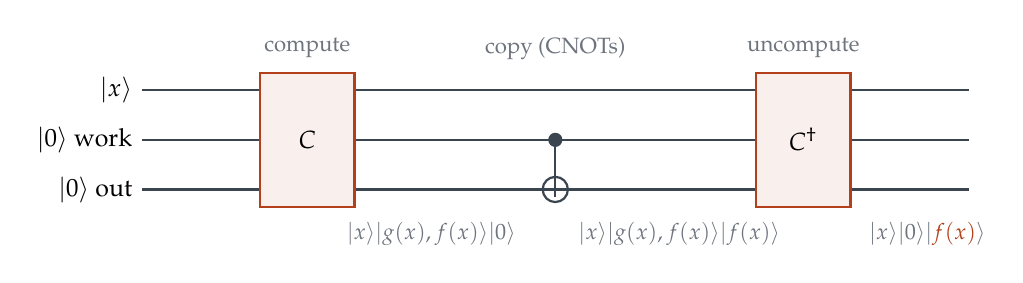
\begin{tikzpicture}[x=10.5mm,y=6.3mm,note/.append style={font=\footnotesize}]
    \foreach \y/\l in {2/{$|x\rangle$},1/{$|0\rangle$ work},0/{$|0\rangle$ out}} {
      \node[lab] at (0,\y) {\l}; \draw[wire] (0,\y) -- (10,\y);}
    \node[op,minimum height=17mm,minimum width=12mm] at (2,1) {$C$};
    \draw[thick,color=body] (5,1) -- (5,0); \node[dot] at (5,1) {}; \oplusat{5}{0}
    \node[op,minimum height=17mm,minimum width=12mm] at (8,1) {$C^\dagger$};
    \node[note] at (3.5,-0.9) {$|x\rangle|g(x),f(x)\rangle|0\rangle$};
    \node[note] at (6.5,-0.9) {$|x\rangle|g(x),f(x)\rangle|f(x)\rangle$};
    \node[note] at (9.5,-0.9) {$|x\rangle|0\rangle|\tgt{f(x)}\rangle$};
    \node[note] at (2,2.85) {compute}; \node[note] at (5,2.85) {copy (CNOTs)}; \node[note] at (8,2.85) {uncompute};
  \end{tikzpicture}
  \vskip2mm
  \begin{columns}[T]
    \begin{column}{0.42\textwidth}
      \blocktitle{The price}
      About twice the gates, plus a register for the copy: a factor 2 in every count that follows.
    \end{column}
    \begin{column}{0.54\textwidth}
      \blocktitle{Where it returns}
      the modular adder's flag; multiply--swap--\emph{un}-multiply; a point addition's second division; the temporary AND
    \end{column}
  \end{columns}
  \resolved{Every scratch register must be back in $|0\rangle$ before the QFT.}
\end{frame}

\setcounter{framenumber}{22}
\begin{frame}{Five levels, each a product of the one below}
  \begin{difficulty}{4}How does ``multiply by $a$ modulo $N$'' become gates? Build it in levels, and check each level exactly before using it.\end{difficulty}
  \centering
  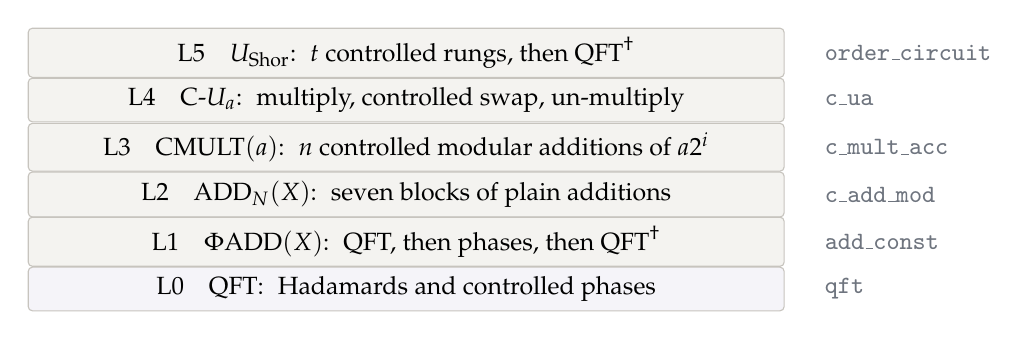
\begin{tikzpicture}[lvl/.style={draw=rulegrey,fill=greybox,rounded corners=1.5pt,minimum width=96mm,
        minimum height=5.3mm,font=\small,anchor=west},
      fn/.style={font=\ttfamily\small,color=subtle,anchor=west}]
    \foreach \i/\l/\f/\c in {
        5/{L5\quad $U_{\text{Shor}}$: \ $t$ controlled rungs, then $\mathrm{QFT}^\dagger$}/order\_circuit/greybox,
        4/{L4\quad $\text{C-}U_a$: \ multiply, controlled swap, un-multiply}/c\_ua/greybox,
        3/{L3\quad $\mathrm{CMULT}(a)$: \ $n$ controlled modular additions of $a2^i$}/c\_mult\_acc/greybox,
        2/{L2\quad $\mathrm{ADD}_N(X)$: \ seven blocks of plain additions}/c\_add\_mod/greybox,
        1/{L1\quad $\Phi\mathrm{ADD}(X)$: \ QFT, then phases, then $\mathrm{QFT}^\dagger$}/add\_const/greybox,
        0/{L0\quad $\mathrm{QFT}$: \ Hadamards and controlled phases}/qft/lavender} {
      \node[lvl,fill=\c] at (0,0.6*\i) {\l};
      \node[fn] at (10,0.6*\i) {\f};}
  \end{tikzpicture}
  \begin{takeaway}Each level is verified exhaustively --- every input, every ancilla back to $|0\rangle$ --- before the next is built on it.\end{takeaway}
\end{frame}

\setcounter{framenumber}{25}
\begin{frame}{L1 --- Draper's adder: addition is a phase}
  In the Fourier basis, qubit $i$ of $\mathrm{QFT}|y\rangle$ carries $e^{2\pi i\,y2^i/2^m}$. Adding $X$ multiplies it by $e^{2\pi i\,X2^i/2^m}$: one phase per qubit, \textbf{no carries}.
  \[
    \Phi\mathrm{ADD}(X)=\mathrm{QFT}^\dagger\Big(\bigotimes_{i=0}^{m-1}P\big(2\pi X2^{i}/2^{m}\big)\Big)\,\mathrm{QFT}
  \]
  \begin{columns}[c]
    \begin{column}{0.44\textwidth}
      \centering\fig[width=0.95\textwidth]{draper3.pdf}
    \end{column}
    \begin{column}{0.52\textwidth}
      {\small $X=3$ on 3 qubits: checked equal to the cyclic shift $y\mapsto y+3 \bmod 8$.}
      \begin{takeaway}To control the adder, control only the phases: the QFT pair cancels when they do not fire.\end{takeaway}
    \end{column}
  \end{columns}
\end{frame}

\setcounter{framenumber}{27}
\begin{frame}{L3--4 --- multiply, swap, un-multiply}
  Shift-and-add, $ax=\sum_i x_i\,(a2^i)$, gives an \emph{out-of-place} product: \ $\mathrm{CMULT}(a)$ is $n$ modular additions of $a2^i$, each controlled by $c$ and $x_i$. Phase estimation needs $U_a$ \emph{in place}:
  \vskip2mm
  \centering
  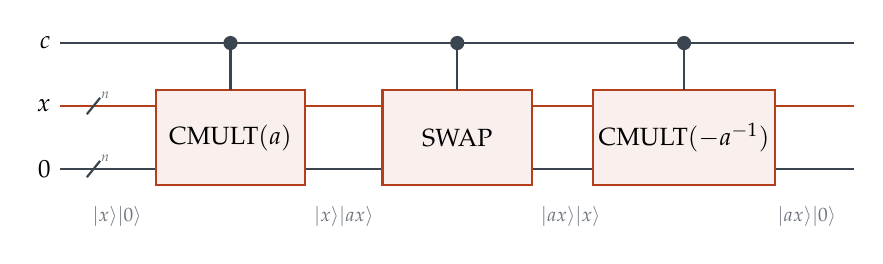
\begin{tikzpicture}[x=12mm,y=8mm]
    \node[lab] at (0,2.2) {$c$}; \draw[wire] (0,2.2) -- (8.4,2.2);
    \node[lab] at (0,1.2) {$x$}; \draw[twire] (0,1.2) -- (8.4,1.2); \bundle{0.35}{1.2}{$n$}
    \node[lab] at (0,0.2) {$0$}; \draw[wire] (0,0.2) -- (8.4,0.2); \bundle{0.35}{0.2}{$n$}
    \foreach \x/\l in {1.8/{$\mathrm{CMULT}(a)$},4.2/{SWAP},6.6/{$\mathrm{CMULT}(-a^{-1})$}} {
      \node[op,minimum width=19mm,minimum height=12mm] at (\x,0.7) {\l};
      \draw[thick,color=body] (\x,2.2) -- (\x,1.46); \node[dot] at (\x,2.2) {};}
    \node[note] at (0.6,-0.55) {$|x\rangle|0\rangle$};
    \node[note] at (3.0,-0.55) {$|x\rangle|ax\rangle$};
    \node[note] at (5.4,-0.55) {$|ax\rangle|x\rangle$};
    \node[note] at (7.9,-0.55) {$|ax\rangle|0\rangle$};
  \end{tikzpicture}
  \vskip1mm
  \raggedright
  \[ \text{C-}U_a=\mathrm{CMULT}(-a^{-1})\cdot\text{C-SWAP}\cdot\mathrm{CMULT}(a) \]
  \begin{takeaway}One rung is $2n$ modular additions and $n$ controlled swaps. The second multiplication only erases the input: uncomputation, made possible by $a^{-1}$.\end{takeaway}
\end{frame}

\setcounter{framenumber}{38}
\begin{frame}{At RSA-2048 size}
  \begin{columns}[T]
    \begin{column}{0.47\textwidth}
      \begin{peachblock}
        \peachtitle{This circuit (verified formulas)}
        8\,194 qubits,\ \ $6.9\times10^{10}$ Toffolis\par
        exact QFTs: $\approx2\times10^{17}$ T\par
        approximate QFTs: $\approx1\times10^{16}$ T\par
        \vskip1mm
        {\small still dominated by rotations}
      \end{peachblock}
    \end{column}
    \begin{column}{0.47\textwidth}
      \begin{greyblock}
        \blocktitle{Reported by the state of the art}
        Gidney--Ekerå 2021: $6\,189$ qubits, $2.7\times10^{9}$ Toffolis --- ripple-carry, windowed.\par
        \vskip1mm
        Gidney 2025: $1\,399$ qubits, $6.5\times10^{9}$ Toffolis --- approximate residue arithmetic.\par
        \vskip1mm
        {\small Physically: $<10^6$ qubits for 5 days, or $\approx94\,000$ for a month.}
      \end{greyblock}
    \end{column}
  \end{columns}
  \resolved{Polynomial but enormous, mostly rotations: Act VII removes them first.}
\end{frame}

% ======================================================================
\act{Part 3 --- How the cost was cut}

\setcounter{framenumber}{46}
\begin{frame}{Toffoli arithmetic: the ripple-carry adder}
  \begin{columns}[c]
    \begin{column}{0.48\textwidth}
      \centering
      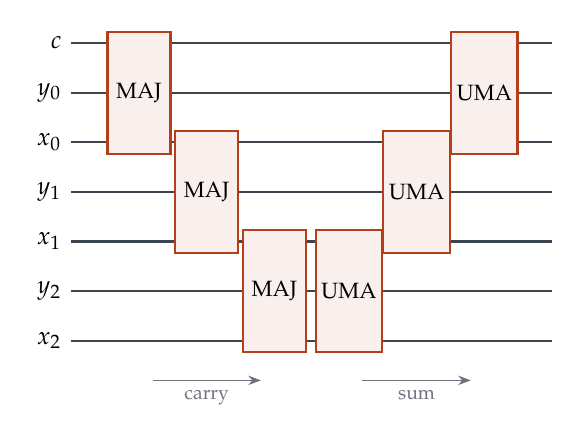
\begin{tikzpicture}[x=8.6mm,y=6.3mm]
        \foreach \y/\l in {6/c,5/y_0,4/x_0,3/y_1,2/x_1,1/y_2,0/x_2} {
          \node[lab] at (0,\y) {$\l$}; \draw[wire] (0,\y) -- (7.1,\y);}
        \foreach \x/\t/\l in {1/6/MAJ,2/4/MAJ,3/2/MAJ,4.1/2/UMA,5.1/4/UMA,6.1/6/UMA}
          \node[op,minimum width=8mm,minimum height=15.5mm,font=\footnotesize] at (\x,\t-1) {\l};
        \draw[-{Stealth[length=1.6mm]},color=subtle] (1.2,-0.8) -- (2.8,-0.8) node[midway,below,note] {carry};
        \draw[-{Stealth[length=1.6mm]},color=subtle] (4.3,-0.8) -- (5.9,-0.8) node[midway,below,note] {sum};
      \end{tikzpicture}
    \end{column}
    \begin{column}{0.48\textwidth}
      Cuccaro et al.: \textbf{MAJ} blocks carry up, \textbf{UMA} blocks write the sum on the way down. Each is one Toffoli and two CNOTs.
      \vskip2mm
      \begin{greyblock}
        $2m$ Toffolis, one carry qubit, \textbf{no rotations}. The seven blocks of the modular adder stay the same; only the adder inside changes.
      \end{greyblock}
    \end{column}
  \end{columns}
\end{frame}

\setcounter{framenumber}{42}
\begin{frame}{One counting qubit: the semiclassical QFT}
  Every rotation of $\mathrm{QFT}^\dagger$ is controlled by a qubit \emph{about to be measured}. Measure it first and control classically: the distribution is unchanged.
  \vskip1mm
  \centering
  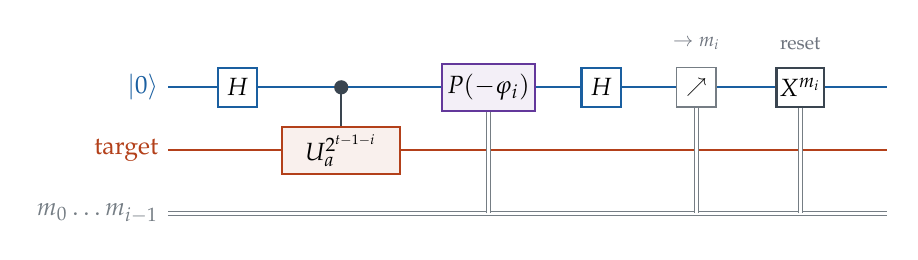
\begin{tikzpicture}[x=11mm,y=8mm]
    \node[lab,color=cblue] at (0,1.6) {$|0\rangle$}; \draw[cwire] (0,1.6) -- (8.3,1.6);
    \node[lab,color=cverm] at (0,0.6) {target}; \draw[twire] (0,0.6) -- (8.3,0.6);
    \node[lab,color=quotebar] at (0,-0.4) {$m_0\dots m_{i-1}$}; \draw[clw] (0,-0.4) -- (8.3,-0.4);
    \node[hop] at (0.8,1.6) {$H$};
    \draw[thick,color=body] (2.0,1.6) -- (2.0,0.9); \node[dot] at (2.0,1.6) {};
    \node[op,minimum width=15mm,minimum height=6mm] at (2.0,0.6) {$U_a^{2^{t-1-i}}$};
    \node[qop,minimum height=6mm] (ph) at (3.7,1.6) {$P(-\varphi_i)$};
    \draw[clw] (3.7,-0.4) -- (ph.south);
    \node[hop] at (5.0,1.6) {$H$};
    \node[meter] (m) at (6.1,1.6) {$\nearrow$};
    \draw[clw] (m.south) -- (6.1,-0.4);
    \node[draw=body,fill=white,thick,minimum size=5mm,font=\small,inner sep=1pt] (x) at (7.3,1.6) {$X^{m_i}$};
    \draw[clw] (7.3,-0.4) -- (x.south);
    \node[note] at (6.1,2.3) {$\to m_i$}; \node[note] at (7.3,2.3) {reset};
  \end{tikzpicture}
  \[ \varphi_i=\pi\sum_{j<i} m_j/2^{\,i-j},\qquad \text{repeat for } i=0,\dots,t-1 \ \text{(heaviest rung first)} \]
  \begin{takeaway}One recycled qubit replaces all $2n$ counting qubits: $4n+2\to2n+3$. The controlled phases become classically controlled single-qubit phases.\end{takeaway}
\end{frame}

\setcounter{framenumber}{50}
\begin{frame}{The temporary AND: uncomputation for free}
  \centering\fig[width=0.97\textwidth]{and_gadget.pdf}\par
  {\scriptsize\color{subtle}Compute with 4 T; uncompute by an $X$-basis measurement and a classically controlled CZ.}
  \vskip1mm
  \begin{columns}[T]
    \begin{column}{0.47\textwidth}
      \blocktitle{Why it works}
      The target starts in $|0\rangle$: 4 T, not 7. An $X$-basis measurement reveals nothing about $a,b$; a Clifford fixes the phase.
    \end{column}
    \begin{column}{0.47\textwidth}
      \blocktitle{What it saves}
      A compute/uncompute pair drops from 14 T to 4: a table lookup costs $3.5\times$ fewer T.
    \end{column}
  \end{columns}
\end{frame}

\setcounter{framenumber}{52}
\begin{frame}{Windowing in three steps}
  \begin{enumerate}\setlength{\itemsep}{1.2mm}
    \item \textbf{A controlled addition is a lookup.} Adding $k$ when $q=1$ is adding $T[q]$ from the table $T=[0,k]$.
    \item \textbf{Address $w$ bits at once.} Window $j$ of $x$ contributes $k\,j\,2^i\bmod N$: tabulate the $2^w$ values and add \textbf{once}, so $n$ additions become $\lceil n/w\rceil$.
    \item \textbf{Fold the control in.} The outer control is one more address bit whose $c=0$ entries are 0: the modular adder needs \textbf{no} control.
  \end{enumerate}
  \centering
  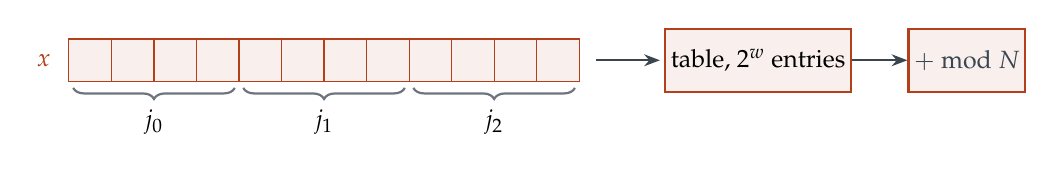
\begin{tikzpicture}[x=5.4mm,y=5.4mm]
    \foreach \i in {0,...,11} \draw[draw=cverm,fill=cverm!8] (\i,0) rectangle (\i+1,1);
    \node[lab,color=cverm] at (-0.2,0.5) {$x$};
    \foreach \w/\c in {0/{$j_0$},4/{$j_1$},8/{$j_2$}} {
      \draw[decorate,decoration={brace,amplitude=4pt,mirror},thick,color=subtle] (\w+0.1,-0.15) -- (\w+3.9,-0.15);
      \node[font=\small] at (\w+2,-0.95) {\c};}
    \draw[-{Stealth[length=2mm]},thick,color=body] (12.4,0.5) -- (13.9,0.5);
    \node[op,minimum height=8mm,anchor=west] (tb) at (14,0.5) {table, $2^w$ entries};
    \draw[-{Stealth[length=2mm]},thick,color=body] (tb.east) -- ++(1.3,0) node[op,minimum height=8mm,anchor=west] {$+$ mod $N$};
  \end{tikzpicture}
  \begin{takeaway}Cost $O\!\big(\tfrac nw(n+2^w)\big)$; $w\approx\log_2n$ balances the terms: $O(n^2/\log n)$, a gain that grows with $n$.\end{takeaway}
\end{frame}

\setcounter{framenumber}{56}
\begin{frame}{Making the lookup cheap: unary iteration}
  \begin{columns}[c]
    \begin{column}{0.5\textwidth}
      \centering
      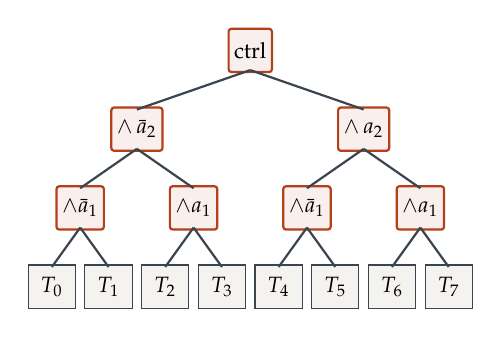
\begin{tikzpicture}[x=7.2mm,y=10mm,nd/.style={draw=cverm,fill=cverm!8,thick,rounded corners=1pt,font=\footnotesize,inner sep=2pt,minimum height=5.5mm},
          lf/.style={draw=body,fill=greybox,font=\footnotesize,inner sep=1.5pt,minimum width=6mm,minimum height=5.5mm}]
        \node[nd] (r) at (3.5,3) {ctrl};
        \node[nd] at (1.5,2) {$\wedge\,\bar a_2$}; \node[nd] at (5.5,2) {$\wedge\,a_2$};
        \foreach \x/\n in {0.5/{$\wedge\bar a_1$},2.5/{$\wedge a_1$},4.5/{$\wedge\bar a_1$},6.5/{$\wedge a_1$}} \node[nd] at (\x,1) {\n};
        \foreach \i in {0,...,7} \node[lf] at (\i,0) {$T_{\i}$};
        \draw[thick,color=body] (3.5,2.75) -- (1.5,2.25); \draw[thick,color=body] (3.5,2.75) -- (5.5,2.25);
        \foreach \a/\b in {1.5/0.5,1.5/2.5,5.5/4.5,5.5/6.5} \draw[thick,color=body] (\a,1.75) -- (\b,1.25);
        \foreach \a/\i in {0.5/0,0.5/1,2.5/2,2.5/3,4.5/4,4.5/5,6.5/6,6.5/7} \draw[thick,color=body] (\a,0.75) -- (\i,0.25);
      \end{tikzpicture}\par
      {\small $m=3$ address bits, $L=8$ entries}
    \end{column}
    \begin{column}{0.46\textwidth}
      The one-hot QROM holds all $2^m$ address states at once. Unary iteration walks the address \textbf{tree} instead, holding only the AND of the current prefix: a node is $\text{parent}\wedge a_i$ (one AND), its sibling the same with one CNOT, and each leaf loads $T[j]$ with CNOTs.
    \end{column}
  \end{columns}
  \begin{peachblock}\peachtitle{Measured}
    $2(L-1)$ Toffolis exactly ($2,6,14,30$ for $m=1..4$) on $m$ ancillas instead of $2^m$ --- $L-1$ with temporary ANDs. At $N=255$, $w=4$: \textbf{59 qubits $\to$ 31}, and the CNOT saving over shift-and-add grows from $1.67\times$ to $2.26\times$.
  \end{peachblock}
\end{frame}

\setcounter{framenumber}{58}
\begin{frame}{Uncomputing a lookup for free}
  \begin{columns}[c]
    \begin{column}{0.5\textwidth}
      \centering
      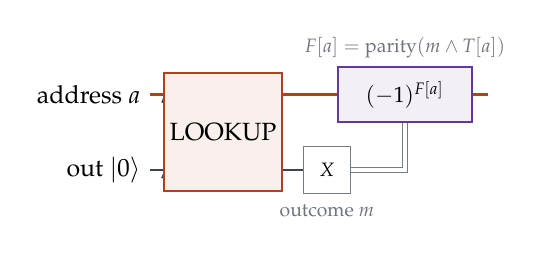
\begin{tikzpicture}[x=6.6mm,y=8mm]
        \node[lab] at (0,1.2) {address $a$}; \draw[twire] (0,1.2) -- (6.5,1.2); \bundle{0.3}{1.2}{$w$}
        \node[lab] at (0,0) {out $|0\rangle$}; \draw[wire] (0,0) -- (3.0,0); \bundle{0.3}{0}{$b$}
        \node[op,minimum width=14mm,minimum height=15mm] at (1.4,0.6) {LOOKUP};
        \node[meter,minimum size=6mm] (m) at (3.4,0) {$X$};
        \draw[clw] (m.east) -- (4.9,0) -- (4.9,0.85);
        \node[qop,minimum width=17mm,minimum height=7mm,font=\footnotesize] at (4.9,1.2) {$(-1)^{F[a]}$};
        \node[note] at (3.4,-0.65) {outcome $m$};
        \node[note] at (4.9,1.95) {$F[a]=\mathrm{parity}(m\wedge T[a])$};
      \end{tikzpicture}
      \vskip2mm
      \raggedright\small
      Measuring the output in $X$ gives a random $m$ and leaves only the phase $(-1)^{m\cdot T[a]}$. A \textbf{phase} lookup costs $O(\sqrt L)$: one-hot the low half of $a$, unary-iterate the high half applying CZ.
    \end{column}
    \begin{column}{0.46\textwidth}
      \centering\footnotesize
      \renewcommand{\arraystretch}{1.12}
      \begin{tabular}{@{}rrrrr@{}}
        \toprule
        $w$ & $L$ & redo & measure & saving \\
        \midrule
        2 & 4 & 6 & 3 & $2.0\times$ \\
        4 & 16 & 30 & 9 & $3.3\times$ \\
        8 & 256 & 510 & 45 & $11.3\times$ \\
        11 & 2\,048 & 4\,094 & 157 & $\mathbf{26.1\times}$ \\
        \bottomrule
      \end{tabular}\par
      {\scriptsize Toffolis. Redo: $2(L-1)$; measure: $2^l-1+2(2^h-1)$,\\ with $l=h=w/2$}
      \vskip2mm
      \begin{greyblock}[fontupper=\small]
        At $w\approx11$, as at cryptographic size, compute $+$ uncompute costs $1.04$ lookups, not 2.
      \end{greyblock}
    \end{column}
  \end{columns}
\end{frame}

{\setbeamertemplate{footline}{\hfill{\scriptsize\color{ink}S1}\hspace*{5mm}\vskip3mm}
\begin{frame}[noframenumbering]{Factoring: what each optimisation bought (1/2)}
  \centering\footnotesize
  \renewcommand{\arraystretch}{1.25}
  \begin{tabular}{@{}>{\raggedright}p{33mm}>{\raggedright}p{52mm}>{\raggedright\arraybackslash\leavevmode\color{cverm}}p{47mm}@{}}
    \toprule
    optimisation & what it removes & \color{ink}measured gain \\
    \midrule
    \textbf{Ripple-carry adders} & every small rotation in the arithmetic & T $-95\%$ ($n=4$) to $-99\%$ ($n=12$) \\
    \textbf{Semiclassical QFT} & the counting register: one qubit, reused & qubits $-41\%$ ($N=21$), $-50\%$ at size \\
    \textbf{Control placement} & controls on blocks that cancel anyway & CNOTs per adder $-92\%$ \\
    \textbf{Temporary AND} & the T cost of uncomputing an AND & T per AND pair $-71\%$ ($14\to4$) \\
    \textbf{Windowing} & most of the modular additions & additions $-75\%$, depth $-70\%$ \\
    \bottomrule
  \end{tabular}\par
  \vskip2mm\raggedright
  {\scriptsize\color{subtle}Free before all of these: precomputed powers ($t$ rungs, not $2^t-1$) and controlled MAJ/UMA ($2n$ controlled gates, not $6n$). Windowing measured at $N=255$, $w=4$.}
\end{frame}}

{\setbeamertemplate{footline}{\hfill{\scriptsize\color{ink}S2}\hspace*{5mm}\vskip3mm}
\begin{frame}[noframenumbering]{Factoring: what each optimisation bought (2/2)}
  \centering\footnotesize
  \renewcommand{\arraystretch}{1.25}
  \begin{tabular}{@{}>{\raggedright}p{33mm}>{\raggedright}p{52mm}>{\raggedright\arraybackslash\leavevmode\color{cverm}}p{47mm}@{}}
    \toprule
    optimisation & what it removes & \color{ink}measured gain \\
    \midrule
    \textbf{Unary iteration} & the lookup's $2^w$ ancillas & lookup qubits $-47\%$ ($59\to31$) \\
    \textbf{Measured uncomputation} & the second lookup & clean-up $-96\%$ ($4\,094\to157$) \\
    \textbf{Nested windows} & exponent rungs and their controls & multiplications $-50\%$ ($8\to4$) \\
    \textbf{Coset representation} & the modular reduction & Toffolis per addition $-67$ to $-74\%$ \\
    \textbf{Approximate QFT} & the smallest rotations & rotations $-34\%$ ($n=8$) \\
    \bottomrule
  \end{tabular}\par
  \vskip1mm\raggedright
  \begin{takeaway}All together at $N=15$: $978\,000$ T $\to$ $\mathbf{42\,600}$ T ($-96\%$), on 17 qubits instead of 18.\end{takeaway}
\end{frame}}

% ======================================================================
\act{Part 4 --- Elliptic-curve keys}

\setcounter{framenumber}{68}
\begin{frame}{Act VIII --- ECDSA keys are discrete logarithms}
  \begin{difficulty}{8}An ECDSA or ECDH key pair is a secret number $\per{d}$ and a public point $Q=\per{d}\,G$ on a curve. Recovering $\per{d}$ from $Q$ is the elliptic-curve discrete logarithm. Does the same circuit solve it?\end{difficulty}
  \vskip2mm
  The points $(x,y)$ with $y^2=x^3+ax+b \pmod p$, plus a point at infinity $O$, form a group. Adding two points:
  \[ \lambda=\frac{y_2-y_1}{x_2-x_1},\qquad x_3=\lambda^2-x_1-x_2,\qquad y_3=\lambda(x_1-x_3)-y_1 . \]
  \begin{takeaway}Point addition needs a modular \textbf{division}. That is the whole cost difference from factoring.\end{takeaway}
\end{frame}

\setcounter{framenumber}{69}
\begin{frame}{A toy curve}
  \begin{columns}[c]
    \begin{column}{0.4\textwidth}
      \centering\fig[width=\textwidth]{curve_p7.pdf}
    \end{column}
    \begin{column}{0.56\textwidth}
      $y^2=x^3+5x+4$ over $\mathbb{F}_7$: nine points and $O$.
      \vskip2mm
      $kP=P+\dots+P$ ($k$ times). \ $G=(0,5)$ has order $r=5$:
      \[ G,\ 2G,\ 3G,\ 4G,\ 5G=O . \]
      The public key $Q=(0,2)=\per{4}\,G$ hides $\per{k=4}$.
    \end{column}
  \end{columns}
\end{frame}

\setcounter{framenumber}{70}
\begin{frame}{Why the key is a hidden period}
  \begin{columns}[T]
    \begin{column}{0.485\textwidth}
      \begin{panel}[equal height group=hp]
        \blocktitle{1. The key hides as a subgroup\vphantom{$L^\perp$}}
        \small\setlength{\abovedisplayskip}{3pt}\setlength{\belowdisplayskip}{3pt}%
        \setlength{\abovedisplayshortskip}{3pt}\setlength{\belowdisplayshortskip}{3pt}%
        With $P$ of prime order $r$ and $Q=[\per{k}]P$:
        \[ f(u,v)=[u]P+[v]Q=[u+\per{k}v]P . \]
        $f$ is constant exactly on the cosets of the hidden subgroup
        \[ \begin{aligned} L&=\{(a,b): a+\per{k}b\equiv0\ (\mathrm{mod}\ r)\}\\ &=\langle(-\per{k},1)\rangle . \end{aligned} \]
        So $f(u-\per{k},\,v+1)=f(u,v)$: a 2-D period; one more $Q$ is $\per{k}$ more copies of $P$.
      \end{panel}
    \end{column}
    \begin{column}{0.485\textwidth}
      \begin{panel}[equal height group=hp]
        \blocktitle{2. Fourier sampling lands in $L^\perp$}
        \small\setlength{\abovedisplayskip}{6pt}\setlength{\belowdisplayskip}{6pt}%
        \setlength{\abovedisplayshortskip}{6pt}\setlength{\belowdisplayshortskip}{6pt}%
        Superpose all $(u,v)$ and evaluate $f$ into a point register:
        \[ \textstyle\sum_{u,v}|u,v\rangle|O\rangle\ \xrightarrow{\,U_f\,}\ \sum_{u,v}|u,v\rangle\,|f(u,v)\rangle . \]
        Inverse QFTs, measure $(s,t)\in L^\perp$:
        \[ \begin{gathered} L^\perp=\{(s,t): -\per{k}s+t\equiv0\}, \\[2pt] t\equiv\per{k}s,\quad \per{k}\equiv t\,s^{-1}\ (\mathrm{mod}\ r)\ \text{ for any } s\neq0 . \end{gathered} \]
      \end{panel}
    \end{column}
  \end{columns}
  \vskip1mm
  \footnotesize\raggedright Toy curve (slide 70): $r=5$, $\per{k}=4$, so $L=\langle(1,1)\rangle$; a shot $(s,t)=(2,3)$ gives ${\per{k}=3\cdot2^{-1}=3\cdot3\equiv4\pmod 5}$. Check $[\per{k}]P=Q$ classically. The oracle is the double-scalar multiplication $[u]P+[v]Q$; everything that follows makes it cheap.
\end{frame}

\setcounter{framenumber}{71}
\begin{frame}{Shor for ECDLP: what changes from factoring}
  \centering\small
  \renewcommand{\arraystretch}{1.24}
  \begin{tabular}{@{}lll@{}}
    \toprule
    & \textbf{factoring $N$} & \textbf{ECDLP, $Q=[\per{k}]P$} \\
    \midrule
    secret & the order $\per{r}$ of $a\bmod N$ & the scalar $\per{k}$; the order $r$ is public \\
    hidden period & in one variable: $a^{x+\per{r}}=a^x$ & in two: $f(u-\per{k},\,v+1)=f(u,v)$ \\
    counting registers & \cnt{one}, $2n$ qubits & \cnt{two}, $n+1$ qubits each \\
    controlled box & \tgt{multiply} by $a^{2^j}\bmod N$ & \tgt{add} the point $[2^j]P$ or $[2^j]Q$ \\
    one box costs & modular additions & additions and a modular \textbf{division} \\
    staying clean & multiply, swap, un-multiply & a second division clears $\lambda$ \\
    read-out & continued fractions, then a gcd & $\per{k}=t\,s^{-1}\bmod r$; check $[\per{k}]P=Q$ \\
    128-bit security & $n=3072$ & $n=256$ \\
    \bottomrule
  \end{tabular}\par
  \vskip1mm
  \raggedright
  \begin{takeaway}Same skeleton, a different box: a point addition costs a division, but the key is $12\times$ shorter. Built here at about $1\,460$ qubits: ECDLP-256 $3.7\times10^7$ Toffolis, RSA-2048 $7.0\times10^9$.\end{takeaway}
\end{frame}

\setcounter{framenumber}{72}
\begin{frame}{Two registers, one accumulator}
  \centering
  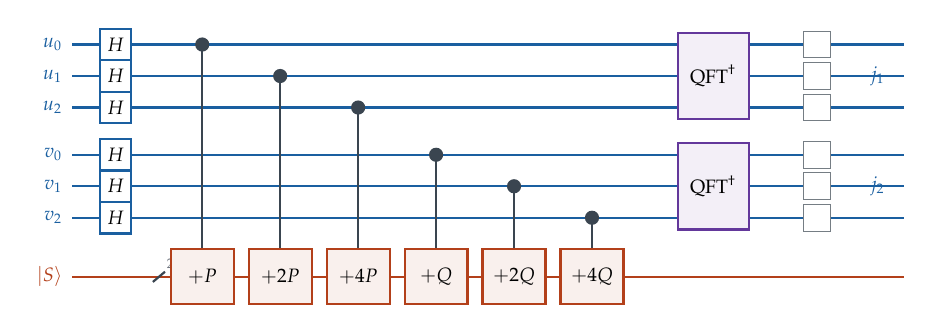
\begin{tikzpicture}[x=11mm,y=5mm]
    \foreach \y/\l in {5/u_0,4.2/u_1,3.4/u_2,2.2/v_0,1.4/v_1,0.6/v_2} {
      \node[lab,color=cblue,font=\scriptsize] at (0,\y) {$\l$};
      \draw[cwire] (0,\y) -- (9.6,\y);
      \node[hop,minimum size=4mm,font=\scriptsize] at (0.5,\y) {$H$};}
    \node[lab,color=cverm,font=\scriptsize] at (0,-0.9) {$|S\rangle$}; \draw[twire] (0,-0.9) -- (9.6,-0.9); \bundle{1.0}{-0.9}{$2n$}
    \foreach \x/\y/\l in {1.5/5/P,2.4/4.2/2P,3.3/3.4/4P,4.2/2.2/Q,5.1/1.4/2Q,6.0/0.6/4Q} {
      \draw[thick,color=body] (\x,\y) -- (\x,-0.45); \node[dot] at (\x,\y) {};
      \node[op,minimum width=8mm,minimum height=7mm,font=\scriptsize] at (\x,-0.9) {$+\l$};}
    \node[qop,minimum height=11mm,minimum width=9mm,font=\scriptsize] at (7.4,4.2) {$\mathrm{QFT}^\dagger$};
    \node[qop,minimum height=11mm,minimum width=9mm,font=\scriptsize] at (7.4,1.4) {$\mathrm{QFT}^\dagger$};
    \foreach \y in {5,4.2,3.4,2.2,1.4,0.6} \node[meter,minimum size=3.4mm] at (8.6,\y) {};
    \node[font=\scriptsize,color=cblue] at (9.3,4.2) {$j_1$}; \node[font=\scriptsize,color=cblue] at (9.3,1.4) {$j_2$};
  \end{tikzpicture}
  \[ \frac{1}{2^m}\sum_{u,v}\cnt{|u\rangle|v\rangle}\;\tgt{|S+uP+vQ\rangle}=\frac{1}{2^m}\sum_{u,v}\cnt{|u\rangle|v\rangle}\;\tgt{|S+(u+\per{k}v)P\rangle} \]
  \raggedright{\small The accumulator depends on $(u,v)$ only through $u+kv\bmod r$; two inverse QFTs turn that into $(j_1,j_2)$. $S$ is a fixed start point, since affine formulas cannot represent $O$ (hit with probability $O(1/p)$).}
\end{frame}

\setcounter{framenumber}{75}
\begin{frame}{Post-processing: the key from $(j_1,j_2)$}
  \begin{columns}[c]
    \begin{column}{0.54\textwidth}
      A peak satisfies $\;j_2\,r/2^m \equiv \per{k}\,(j_1\,r/2^m) \pmod r$. Round, and divide:
      \[ a_i=\mathrm{round}\big(j_i\,r/2^m\big),\qquad \per{k}=a_2\,a_1^{-1}\bmod r . \]
      Every shot votes; the winner is checked with $kG=Q$.
      \vskip2mm
      {\small Code: \texttt{ec\_classical.ecdlp\_postprocess} (backup). It also tries $\pm1$ around the rounding when $2^m$ is not a multiple of $r$ (Ekerå).}
    \end{column}
    \begin{column}{0.42\textwidth}
      \centering\fig[width=\textwidth]{ecdlp_votes.pdf}
    \end{column}
  \end{columns}
  \begin{takeaway}$k=4$ takes 42\% of the vote, against 13--16\% for each wrong key: a signal, not luck.\end{takeaway}
\end{frame}

\setcounter{framenumber}{76}
\begin{frame}{One point addition is eleven reversible steps}
  \begin{columns}[c]
    \begin{column}{0.54\textwidth}
      \centering\fig[width=\textwidth]{padd_steps.pdf}
    \end{column}
    \begin{column}{0.42\textwidth}
      \blocktitle{In place, no garbage}
      Step 3 divides to get $\lambda$. Step 4 clears $y$, since $x\lambda=y$. Step 8 is the \emph{same} division; by then $y/x=\lambda$ again, so it \textbf{clears} $\lambda$ --- uncomputation.
      \vskip2mm
      {\small A division is Kaliski's binary extended-Euclid inversion: $2n$ rounds of shifts and subtractions.}
    \end{column}
  \end{columns}
  \begin{takeaway}The two divisions are 80\% of the 2\,744 Toffolis of one addition ($p=7$).\end{takeaway}
\end{frame}

\setcounter{framenumber}{78}
\begin{frame}{Making ECDLP fast: one optimisation per level}
  \centering\footnotesize
  \renewcommand{\arraystretch}{1.12}
  \begin{tabular}{@{}lll@{}}
    \toprule
    level & optimisation & measured on a fixed task \\
    \midrule
    L0 & temporary AND (Gidney) & $2.50\times$ fewer T over one inversion \\
    L1 & Gidney adder, copy-then-add control [106] & controlled add $128\to63$ Toffolis ($n=32$) \\
    L2 & top-bit, pseudo-Mersenne reduction [1128] & doubling $25\to4$ Toffolis, 3.1\% failures \\
    L3 & Montgomery on a carry-save tree [106] & depth $\div2.0$ ($n=16$) \\
    L3 & Kaliski: no counter, late reduction [106] & $-29\%$ Toffolis, $-41\%$ depth ($n=12$) \\
    L3 & Euclidean dialog and replay [1128] & $-54\%$ Toffolis, $-43\%$ qubits ($p=61$) \\
    L4 & Jacobian coordinates [106] & $-45\%$ Toffolis, $3n$ garbage qubits \\
    L5 & windows, zig-zag, one control qubit & $514\to34$ additions at $n=256$ \\
    \bottomrule
  \end{tabular}
  \vskip2mm
  \raggedright
  {\small [106] Kim et al., eprint 2026/106; [1128] Schrottenloher, eprint 2026/1128. Each variant is re-checked against the classical model inside the benchmark before it is counted; approximate ones record a failure rate.}
\end{frame}

\setcounter{framenumber}{93}
\begin{frame}{L5: window by window --- look up, add, unlook up}
  \small Cut each scalar into $\ell=\lceil n/w\rceil$ windows of $w$ bits, $u=\sum_{j<\ell}u_j2^{jw}$, and the oracle becomes a sum of table entries:
  \[ [u]P+[v]Q=\sum_{j<\ell}[u_j]P_j+\sum_{j<\ell}[v_j]Q_j,\qquad P_j=[2^{jw}]P,\quad Q_j=[2^{jw}]Q . \]
  \begin{columns}[c]
    \begin{column}{0.47\textwidth}
      \centering
      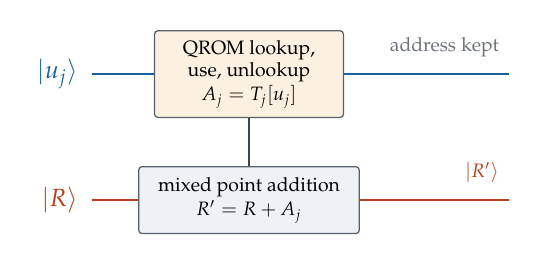
\begin{tikzpicture}[x=1mm,y=1mm]
        \draw[cwire] (11,16) -- (64,16); \node[lab,color=cblue] at (10.5,16) {$|u_j\rangle$};
        \draw[twire] (11,0) -- (64,0); \node[lab,color=cverm] at (10.5,0) {$|R\rangle$};
        \node[bxl,minimum width=24mm,minimum height=11mm] (L) at (31,16) {QROM lookup,\\use, unlookup\\[0.3mm] $A_j=T_j[u_j]$};
        \node[bxa,minimum width=28mm,minimum height=8.5mm] (A) at (31,0) {mixed point addition\\[0.3mm] $R'=R+A_j$};
        \draw[thick,color=body] (L.south) -- (A.north);
        \node[note,anchor=south east] at (64,17) {address kept};
        \node[note,anchor=south east,color=cverm] at (64,1) {$|R'\rangle$};
      \end{tikzpicture}
    \end{column}
    \begin{column}{0.49\textwidth}
      \small The table $T_j[i]=[i\,2^{jw}]P$ has $2^w$ entries, all computed classically before the run. The window is a coherent \textbf{address}, not a control bit: the circuit loads the point it selects, adds it, and erases it.
    \end{column}
  \end{columns}
  \vskip2mm
  \centering\footnotesize
  $|z\rangle|0\rangle_A|R\rangle\xrightarrow{\text{lookup}}|z\rangle|T_j[z]\rangle_A|R\rangle\xrightarrow{\text{add}}|z\rangle|T_j[z]\rangle_A|R+T_j[z]\rangle\xrightarrow{\text{unlookup}}|z\rangle|0\rangle_A|R+T_j[z]\rangle$\par
  \vskip1mm
  {\scriptsize $n=256$, $w=16$: 16 windows per scalar, 32 such updates}
\end{frame}

{\setbeamertemplate{footline}{\hfill{\scriptsize\color{ink}S3}\hspace*{5mm}\vskip3mm}
\begin{frame}[noframenumbering]{Elliptic curves at toy size: what each level bought}
  \centering\footnotesize
  \renewcommand{\arraystretch}{1.1}
  \begin{tabular}{@{}>{\raggedright}p{42mm}>{\raggedright}p{44mm}>{\raggedright\arraybackslash\leavevmode\color{cverm}}p{46mm}@{}}
    \toprule
    level and technique & what it does & \color{ink}measured gain \\
    \midrule
    \textbf{L0} temporary AND & 4-T ANDs in the inversion & T $-60\%$ \\
    \textbf{L1} Gidney adder & $n-1$ ANDs, control on a copy & controlled add $-51\%$ \\
    \textbf{L2} pseudo-Mersenne & subtract $p$: clear a bit, add $f$ & doubling $-84\%$ \\
    \textbf{L3} carry-save Montgomery & one compressor tree & depth $-50\%$ ($4\times$ qubits) \\
    \textbf{L3} Kaliski, late reduction & reduce once, at the end & Toffolis $-29\%$, depth $-41\%$ \\
    \textbf{L3} Euclidean dialog & 2 bits per round, replayed & Toffolis $-54\%$, qubits $-43\%$ \\
    \textbf{L4} Jacobian coordinates & no division at all & Toffolis $-45\%$ ($3n$ garbage) \\
    \textbf{L5} windows, zig-zag & 16-bit windows & additions $-93\%$ ($514\to34$) \\
    \bottomrule
  \end{tabular}\par
  \vskip1mm\raggedright
  \begin{takeaway}Halving a point addition is worth half as much as running fifteen times fewer of them.\end{takeaway}
\end{frame}}

\setcounter{framenumber}{106}
\begin{frame}{At 128-bit security}
  \begin{columns}[c]
    \begin{column}{0.57\textwidth}
      \centering\fig[width=\textwidth]{rsa_vs_ecc.pdf}
    \end{column}
    \begin{column}{0.4\textwidth}
      \blocktitle{Toffolis}
      $(3072/256)^3=1\,728$, and $1\,728/6.7\approx260$: \par
      this repo's circuits $\approx270\times$ fewer for P-256; minimal-width literature $148\times$; optimised literature $\approx180\times$.
      \vskip2mm
      \blocktitle{Qubits}
      depend on the construction: $2.6\times$ fewer in like-for-like circuits, but RSA-2048 now fits in $\approx1\,400$ (Gidney 2025).
    \end{column}
  \end{columns}
\end{frame}

\setcounter{framenumber}{108}
\begin{frame}{What it means}
  \begin{peachblock}
    \peachtitle{Elliptic curves are the cheaper target}
    The short key that makes ECC efficient classically makes it the easier quantum target: two orders of magnitude fewer Toffolis at the same security. Optimised: $4$--$9\times10^{7}$ for a 256-bit curve (Google, IonQ 2026) against $6.5\times10^{9}$ for RSA-2048 (Gidney 2025).
  \end{peachblock}
  \vskip3mm
  \begin{columns}[T]
    \begin{column}{0.47\textwidth}
      \blocktitle{Key exchange (ECDH)}
      Traffic recorded today can be decrypted later: \emph{harvest now, decrypt later}.
    \end{column}
    \begin{column}{0.47\textwidth}
      \blocktitle{Signatures (ECDSA)}
      Once a large machine exists, anyone can forge. Migrate to ML-KEM and ML-DSA (FIPS 203, 204).
    \end{column}
  \end{columns}
  \resolved{ECDSA falls first: same cubic cost, a 12$\times$ shorter key, a $\approx7\times$ heavier group operation --- 20 minutes against 5 days on the same hardware.}
\end{frame}

% ======================================================================
\act{Part 5 --- Where things stand in 2026}

{\setbeamertemplate{footline}{\hfill{\scriptsize\color{ink}N13}\hspace*{5mm}\vskip3mm}
\begin{frame}[noframenumbering]{Choosing the code distance from the error budget}
  \begin{columns}[T,onlytextwidth]
    \begin{column}{0.53\textwidth}
      \footnotesize\setlength{\abovedisplayskip}{2pt}\setlength{\belowdisplayskip}{2pt}%
      \textbf{1. Budget.} A run fails if any qubit fails in any round:
      \[ P_{\rm fail}\approx P_L\times\text{qubits}\times\text{rounds}. \]
      ECDLP-256: $1.4\times10^{12}$ qubit-rounds; RSA-2048: $7\times10^{13}$. With $P_L=10^{-15}$ they fail $0.1\%$ and $7\%$ of the time.\par\vskip1mm
      \textbf{2. Scaling.} $P_L(d)\approx0.1\,(p/p_{\rm th})^{(d+1)/2}$, $p_{\rm th}\approx1.2\%$: each $d\to d+2$ divides it by ${\approx}12$ at $p=10^{-3}$.\par\vskip1mm
      \textbf{3. Solve.} $\dfrac{d+1}{2}\ge\dfrac{\log(0.1/P_L)}{\log(p_{\rm th}/p)}=\dfrac{14}{1.09}$, so $d=25$.
    \end{column}
    \begin{column}{0.44\textwidth}
      \centering\footnotesize
      \renewcommand{\arraystretch}{1.2}
      \begin{tabular}{@{}rrr@{}}
        \toprule
        physical $p$ & $d$ & per logical \\
        \midrule
        $10^{-3}$ & $25$ & $1\,352$ \\
        $5\times10^{-4}$ & $21$ & $968$ \\
        $10^{-4}$ & $13$ & $392$ \\
        \bottomrule
      \end{tabular}\par
      \vskip1.5mm\raggedright
      {\scriptsize Physical qubits per working logical qubit, $2(d+1)^2$, at $P_L=10^{-15}$.}
    \end{column}
  \end{columns}
  \vskip1mm
  \begin{takeaway}$d$ grows with the log of the run; a $10\times$ better $p$ cuts qubits per logical qubit $3.5\times$.\end{takeaway}
\end{frame}}

{\setbeamertemplate{footline}{\hfill{\scriptsize\color{ink}N12}\hspace*{5mm}\vskip3mm}
\begin{frame}[noframenumbering]{From logical to physical qubits: the recipe}
  \begin{columns}[T,onlytextwidth]
    \begin{column}{0.5\textwidth}
      \footnotesize
      At $p=10^{-3}$, a $1\,\mu$s cycle, $10\,\mu$s reaction:\par\vskip1mm
      \textbf{1.} Pick $d$ with $0.1\,(p/0.0122)^{(d+1)/2}\le10^{-15}$: $d=25$.\par\vskip0.6mm
      \textbf{2.} Working logical qubit: $2(d+1)^2=\mathbf{1\,352}$.\par\vskip0.6mm
      \textbf{3.} Idle logical qubit (yoked storage): ${\approx}\mathbf{430}$.\par\vskip0.6mm
      \textbf{4.} Factories $+$ workspace: $\mathbf{170\,352}$.\par\vskip0.6mm
      \textbf{5.} One CCZ every $\mathbf{25}\,\mu$s: time $=$ Toffolis $\times25\,\mu$s.
    \end{column}
    \begin{column}{0.47\textwidth}
      \centering\footnotesize
      \renewcommand{\arraystretch}{1.2}
      \begin{tabular}{@{}lrr@{}}
        \toprule
        & ECDLP-256 & RSA-2048 \\
        \midrule
        working logical & $1\,457$ & $131$ \\
        idle logical & -- & $1\,280$ \\
        Toffolis & $3.68\times10^{7}$ & $6.5\times10^{9}$ \\
        \textbf{physical} & $\mathbf{2\,140\,216}$ & $\mathbf{897\,864}$ \\
        \textbf{time} & \textbf{15 min} & \textbf{4.96 d} \\
        \bottomrule
      \end{tabular}\par
      \vskip1mm\raggedright
      {\scriptsize $1\,457\times1\,352+170\,352$; \ $1\,280\times430+131\times1\,352+170\,352$. RSA: $12.07$ h $\times$ 9.2 shots $=4.63$ d, $\div\,93\%$ error-free.}
    \end{column}
  \end{columns}
  \vskip1mm
  {\scriptsize\color{subtle}Gidney 2025's model (Sec.~3.2), in \texttt{shor\_qiskit/physical.py}; it reproduces the paper's headline.}
  \begin{takeaway}Physical $\approx$ logical $\times\,1\,352+170\,352$; runtime $\approx$ Toffolis $\times\,25\,\mu$s.\end{takeaway}
\end{frame}}

\setcounter{framenumber}{156}
\begin{frame}{The logical frontier, September 2026}
  \begin{columns}[c]
    \begin{column}{0.58\textwidth}
      \centering
      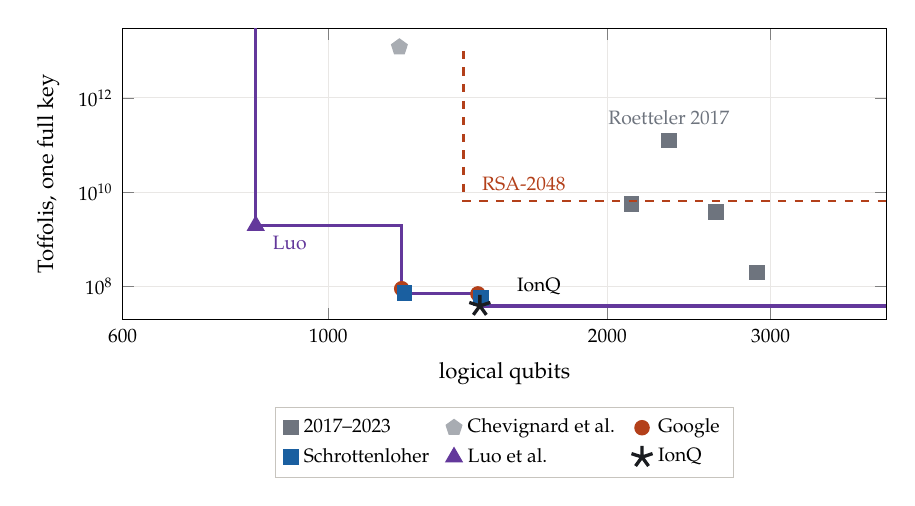
\begin{tikzpicture}
      \begin{axis}[scale only axis,width=0.8\linewidth,height=3.7cm,xmode=log,ymode=log,xmin=600,xmax=4000,ymin=2e7,ymax=3e13,
        xlabel={logical qubits},ylabel={Toffolis, one full key},xtick={600,1000,2000,3000},xticklabels={600,1000,2000,3000},
        grid=both,clip mode=individual,
        legend style={at={(0.5,-0.3)},anchor=north,legend columns=3,/tikz/every even column/.append style={column sep=4pt}}]
        \addplot[very thick,cpurple,forget plot] coordinates {(835,3e13) (835,1.97e9) (1200,1.97e9) (1200,9e7) (1208,9e7) (1208,7.24e7) (1450,7.24e7) (1450,7e7) (1457,7e7) (1457,3.9e7) (4000,3.9e7)};
        \addplot[only marks,mark=square*,mark size=2.6pt,subtle] coordinates {(2330,1.26e11) (2124,5.7e9) (2619,3.8e9) (2900,2e8)};\addlegendentry{2017--2023}
        \addplot[only marks,mark=pentagon*,mark size=3pt,subtle!60] coordinates {(1193,1.19e13)};\addlegendentry{Chevignard et al.}
        \addplot[only marks,mark=*,mark size=2.6pt,cverm] coordinates {(1200,9e7) (1450,7e7)};\addlegendentry{Google}
        \addplot[only marks,mark=square*,mark size=2.6pt,cblue] coordinates {(1208,7.24e7) (1462,5.76e7)};\addlegendentry{Schrottenloher}
        \addplot[only marks,mark=triangle*,mark size=3.4pt,cpurple] coordinates {(835,1.97e9)};\addlegendentry{Luo et al.}
        \addplot[only marks,mark=star,mark size=4pt,very thick,ink] coordinates {(1457,3.9e7)};\addlegendentry{IonQ}
        \addplot[thick,cverm,dashed,forget plot] coordinates {(1399,1e13) (1399,6.5e9) (6189,6.5e9)};
        \node[font=\scriptsize,cverm,anchor=south west] at (axis cs:1430,6.5e9) {RSA-2048};
        \node[font=\scriptsize,cpurple,anchor=north west] at (axis cs:850,1.9e9) {Luo};
        \node[font=\scriptsize,anchor=south west] at (axis cs:1560,4.2e7) {IonQ};
        \node[font=\scriptsize,subtle,anchor=south] at (axis cs:2330,1.7e11) {Roetteler 2017};
      \end{axis}
      \end{tikzpicture}
    \end{column}
    \begin{column}{0.38\textwidth}
      \small
      \blocktitle{ECDLP-256 frontier (purple)}
      Luo et al.\ $(835,\,2.0\times10^9)$ $\to$ Google $(1\,200,\,9\times10^7)$ $\to$ Schrottenloher $(1\,208,\,7.2\times10^7)$ $\to$ Google $(1\,450,\,7\times10^7)$ $\to$ IonQ $(1\,457,\,3.9\times10^7)$.
      \vskip2mm
      \blocktitle{RSA-2048 (dashed)}
      Gidney 2025 $(1\,399,\,6.5\times10^9)$; Gidney--Ekerå $(6\,189,\,2.7\times10^9)$. The 2026 progress on RSA was in the machines, not the arithmetic.
    \end{column}
  \end{columns}
\end{frame}

\setcounter{framenumber}{163}
\begin{frame}{Act XII --- from the papers as printed to below IonQ's count}
  \begin{difficulty}{12}Act VIII built eprints 2026/106 and 2026/1128 as printed: $2.6$M Toffolis per point addition. IonQ reports $1.39$M on $1\,457$ qubits. Where is the factor 2?\end{difficulty}
  \centering\small
  \renewcommand{\arraystretch}{1.05}
  \begin{tabular}{@{}lrr@{}}
    \toprule
    one windowed point addition, $n=256$, $w=16$ & before & after \\
    \midrule
    two in-place multiplications & 3\,910\,552 & 1\,441\,130 \\
    square-subtract & 1\,050\,623 & 79\,160 \\
    table lookups & 1\,310\,700 & 197\,364 \\
    five modular additions & 5\,115 & 5\,115 \\
    \midrule
    total & 6\,276\,990 & \textbf{1\,722\,769} \\
    whole ECDLP-256 ($34\to28$ additions) & 213M & \textbf{48M} \\
    \bottomrule
  \end{tabular}
  \begin{takeaway}$3.6\times$ per addition from three changes: measured uncomputation, a cheaper GCD, a squarer.\end{takeaway}
\end{frame}

\setcounter{framenumber}{206}
\begin{frame}{Act XII in plain words (1/3)}
  \centering\footnotesize
  \renewcommand{\arraystretch}{1.15}
  \begin{tabular}{@{}>{\raggedright}p{30mm}>{\raggedright}p{63mm}>{\raggedright\arraybackslash\leavevmode\color{cverm}}p{40mm}@{}}
    \toprule
    optimisation & what it does & \color{ink}what it bought \\
    \midrule
    \textbf{Measured lookup uncomputation} & ten recomputed lookups become three loads and one shared phase repair & $1.31$M $\to197\,364$ Toffolis per addition \\
    \textbf{Conditionally inverted GCD} & keep both values odd, so each step is one uncontrolled adder between rows of CNOTs & in-place multiplication $1.96\to0.72$M \\
    \textbf{Squarer and fold} & squaring as unconditional signed subtractions, reduced with the shape of $p$ & square-subtract $1.05$M $\to79\,160$ \\
    \textbf{Carry-is-flag adder (IonQ)} & add with carry-out; the carry decides the reduction and is cleared by a measurement and a phase fix & replay step $712\to352$; addition $1.71\to1.44$M \\
    \textbf{37 careful steps, own replay} & the one sum the carry misses ($x+y=p$) occurs early; multiplication gets its own replay & exact on every test; $569\,600\to307\,574$ \\
    \bottomrule
  \end{tabular}
  \par\vskip1mm{\scriptsize\color{subtle}All at $n=256$, $w=16$, per windowed point addition unless stated.}
\end{frame}

\setcounter{framenumber}{207}
\begin{frame}{Act XII in plain words (2/3)}
  \centering\footnotesize
  \renewcommand{\arraystretch}{1.15}
  \begin{tabular}{@{}>{\raggedright}p{30mm}>{\raggedright}p{63mm}>{\raggedright\arraybackslash\leavevmode\color{cverm}}p{40mm}@{}}
    \toprule
    optimisation & what it does & \color{ink}what it bought \\
    \midrule
    \textbf{Signed windows} & read each window as $\pm d$, look up $|d|$, negate $y$ for the sign & $2^{15}$-entry tables, no $O$; $4.6\%$ below IonQ \\
    \textbf{Peak chasing} & free the scratch of whichever step sets the peak; pack the record, share registers & $2\,233\to1\,457$ qubits, no extra Toffoli \\
    \textbf{SELECT-SWAP} & load $2^k$ words at once and route one with Fredkins, on qubits idle at that moment & $1.327\to1.311$M executed at $1\,457$ qubits \\
    \textbf{Lean cells} & CDKM adders, a 1-ancilla comparator, chunked tests, a constant adder with a borrowed increment & $2\,251\to1\,246$ qubits, $1.71\to2.82$M Toffolis \\
    \textbf{Controlled CDKM at $3n$} & carries computed uncontrolled; only the sum write is controlled & $4n\to3n$ Toffolis \\
    \bottomrule
  \end{tabular}
\end{frame}

{\setbeamertemplate{footline}{\hfill{\scriptsize\color{ink}S4}\hspace*{5mm}\vskip3mm}
\begin{frame}[noframenumbering]{secp256k1 at full size: what each change bought}
  \centering\footnotesize
  \renewcommand{\arraystretch}{1.1}
  \begin{tabular}{@{}>{\raggedright}p{50mm}>{\raggedright}p{58mm}>{\raggedright\arraybackslash\leavevmode\color{cverm}}p{24mm}@{}}
    \toprule
    one point addition, $n=256$, $w=16$ & before $\to$ after & \color{ink}gain \\
    \midrule
    Measured lookup clean-up & lookups $1.31$M $\to197$k Toffolis & $-85\%$ \\
    Inverted-step GCD (IonQ) & multiplication $1.96\to0.72$M & $-63\%$ \\
    Squarer and fold & square-subtract $1.05$M $\to79$k & $-92\%$ \\
    \textbf{Three changes together} & $\mathbf{6.28\to1.72}$\textbf{M Toffolis} & $\mathbf{-73\%}$ \\
    Carry-is-flag adder (IonQ) & replay step $712\to352$ & $-51\%$ \\
    Signed windows & tables $2^{16}\to2^{15}$ entries & $-7\%$ \\
    Peak chasing and sharing & qubits $2\,233\to1\,457$ & $-35\%$ \\
    SELECT-SWAP, $3x$ lookup & $1.327\to1.311$M executed & $-1.2\%$ \\
    \bottomrule
  \end{tabular}\par
  \vskip1mm\raggedright
  \begin{takeaway}$1.31$M executed Toffolis per addition on $1\,457$ qubits, $5.9\%$ below IonQ. Whole ECDLP-256: $213$M $\to$ $\mathbf{37.1}$\textbf{M} ($-83\%$).\end{takeaway}
\end{frame}}

{\setbeamertemplate{footline}{\hfill{\scriptsize\color{ink}S5}\hspace*{5mm}\vskip3mm}
\begin{frame}[noframenumbering]{Other trade-offs: fewer qubits, or less depth}
  \centering\footnotesize
  \renewcommand{\arraystretch}{1.25}
  \begin{tabular}{@{}>{\raggedright}p{50mm}>{\raggedright}p{44mm}>{\raggedright\arraybackslash\leavevmode\color{cverm}}p{38mm}@{}}
    \toprule
    one point addition, $n=256$ & gain & \color{ink}price \\
    \midrule
    \textbf{Lean cells}: CDKM adders, a 1-ancilla comparator, a borrowed increment & qubits $2\,251\to1\,246$ ($-45\%$) & Toffolis $1.71\to2.82$M ($+65\%$) \\
    \textbf{Register-shared Euclid} (Luo et al.): no record kept & qubits $1\,246\to1\,107$ & $30\times$ the Toffolis \\
    \textbf{Three field registers}: measure $y$ away, repair the phase & $851$ qubits & $85.2$M Toffolis per addition \\
    \textbf{Carry-lookahead adders}, controls fanned out & Toffoli depth $1.50\to0.39$M ($-74\%$) & $4.6\times$ the Toffolis \\
    \bottomrule
  \end{tabular}\par
  \vskip1mm\raggedright
  \begin{takeaway}The headline circuit sits at $1\,457$ qubits; going narrower or shallower is possible, and it costs Toffolis.\end{takeaway}
\end{frame}}

\setcounter{framenumber}{205}
\begin{frame}{The built frontier}
  \begin{columns}[c]
    \begin{column}{0.64\textwidth}
      \centering
      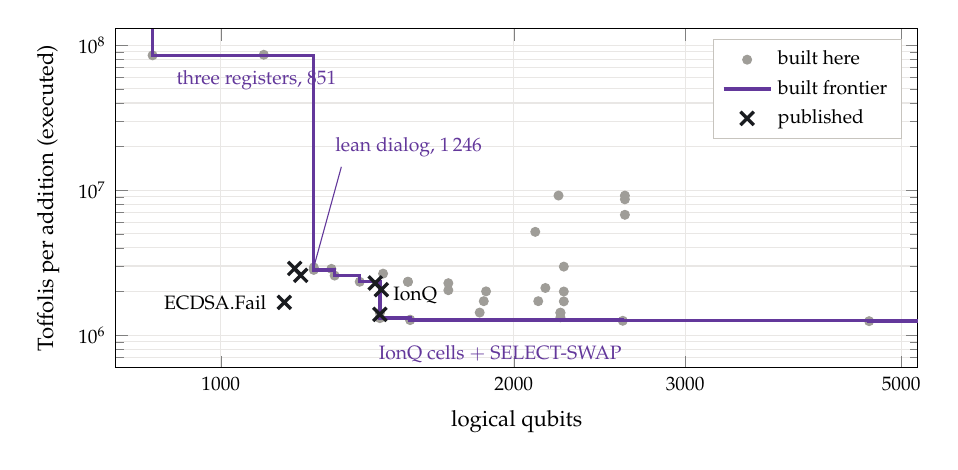
\begin{tikzpicture}
      \begin{axis}[scale only axis,width=0.84\linewidth,height=4.3cm,xmode=log,ymode=log,xmin=780,xmax=5200,ymin=6e5,ymax=1.3e8,
        xlabel={logical qubits},ylabel={Toffolis per addition (executed)},xtick={1000,2000,3000,5000},xticklabels={1000,2000,3000,5000},
        grid=both,clip mode=individual,
        legend style={at={(0.98,0.97)},anchor=north east}]
        \addplot[only marks,mark=*,mark size=1.6pt,rulegrey!80!black] coordinates {
          (851,85204396) (1107,86033905) (1246,2821091) (1246,2853603) (1246,2935857) (1299,2868531) (1309,2577278)
          (1389,2335990) (1457,1310693) (1457,1326821) (1457,1424871) (1468,2659019) (1557,2333400) (1557,2338844)
          (1565,1271269) (1565,1278949) (1713,2042914) (1713,2284770) (1845,1432285) (1863,1716514) (1873,2006184)
          (2104,5163617) (2119,1716514) (2155,2117534) (2223,9189792) (2233,1328915) (2233,1426965) (2233,1430352)
          (2251,1711194) (2251,2000864) (2251,2972327) (2588,1256933) (2601,6769556) (2601,8655996) (2601,9184472)
          (4635,1249765)};\addlegendentry{built here}
        \addplot[very thick,cpurple] coordinates {(851,1.3e8) (851,85204396) (1246,85204396) (1246,2821091) (1309,2821091) (1309,2577278) (1389,2577278) (1389,2335990) (1457,2335990) (1457,1310693) (1565,1310693) (1565,1271269) (2588,1271269) (2588,1256933) (4635,1256933) (4635,1249765) (5200,1249765)};\addlegendentry{built frontier}
        \addplot[only marks,mark=x,mark size=3.4pt,very thick,ink] coordinates {(1208,2588963) (1462,2060646) (1191,2888147) (1441,2293760) (1457,1392608) (1162,1684161)};\addlegendentry{published}
        \node[font=\scriptsize,cpurple,anchor=north west] at (axis cs:880,7.8e7) {three registers, 851};
        \draw[cpurple,thin] (axis cs:1246,2.95e6) -- (axis cs:1330,1.45e7) node[anchor=south west,font=\scriptsize,xshift=-2mm] {lean dialog, 1\,246};
        \node[font=\scriptsize,cpurple,anchor=north west] at (axis cs:1420,1.0e6) {IonQ cells $+$ SELECT-SWAP};
        \node[font=\scriptsize,anchor=south west] at (axis cs:1470,1.4e6) {IonQ};
        \node[font=\scriptsize,anchor=east] at (axis cs:1140,1.68e6) {ECDSA.Fail};
      \end{axis}
      \end{tikzpicture}
    \end{column}
    \begin{column}{0.33\textwidth}
      \small Grey: every circuit built at $n=256$ (secp256k1's prime); Qualtran counts the same Toffolis. Crosses: [1128], Google, IonQ, ECDSA.Fail.
      \vskip2mm
      The frontier ends at IonQ's cells with SELECT-SWAP: 1\,457 qubits, 1.31M executed --- below IonQ's own point.
    \end{column}
  \end{columns}
  \resolved{The factor 2 between [1128] and IonQ is three ideas, all reproduced.}
\end{frame}

{\setbeamertemplate{footline}{\hfill{\scriptsize\color{ink}S0}\hspace*{5mm}\vskip3mm}
\begin{frame}[noframenumbering]{What the optimisations in the repo bought}
  \centering\footnotesize
  \renewcommand{\arraystretch}{1.3}
  \begin{tabular}{@{}>{\raggedright\bfseries}p{30mm}>{\raggedright\arraybackslash}p{68mm}>{\raggedright\arraybackslash\leavevmode\color{cverm}}p{34mm}@{}}
    \toprule
    & \mdseries biggest single gains & \color{ink}overall \\
    \midrule
    Factoring & ripple-carry adders: T $-95$ to $-99\%$\newline one counting qubit: qubits $-41$ to $-50\%$\newline measured clean-up of a lookup: $-96\%$ & T $-96\%$ at $N=15$ \\
    Elliptic curves, toy size & Euclidean dialog: Toffolis $-54\%$, qubits $-43\%$\newline pseudo-Mersenne doubling: $-84\%$\newline 16-bit windows: point additions $-93\%$ & each level measured on a fixed task \\
    secp256k1, $n=256$ & three changes: $6.28\to1.72$M per addition ($-73\%$)\newline peak chasing: $2\,233\to1\,457$ qubits ($-35\%$)\newline $1.31$M per addition, $5.9\%$ below IonQ & whole ECDLP-256: $213\to37.1$M ($-83\%$) \\
    \bottomrule
  \end{tabular}\par
  \vskip1mm\raggedright
  \begin{takeaway}Every number is a count the repo measured on circuits it built, each optimisation switched on and off.\end{takeaway}
\end{frame}}

\setcounter{framenumber}{210}
\begin{frame}{Seven things to keep}
  \begin{enumerate}
    \setlength{\itemsep}{1.2mm}
    \item \textbf{Shor is phase estimation of a group operation.} The quantum part is short; the cost is reversible arithmetic.
    \item \textbf{Uncomputation is mandatory.} Garbage that records $x$ erases the peaks.
    \item \textbf{The price is T gates.} A Toffoli costs 7; a small rotation $\approx3\log_2(1/\varepsilon)$.
    \item \textbf{Optimise in order.} Remove rotations, then the counting register, then additions.
    \item \textbf{Elliptic curves fall first.} Same $\Theta(n^3)$, a 12$\times$ shorter key: $150$--$270\times$ cheaper.
    \item \textbf{Gates are Hamiltonians.} Universality is a Lie-bracket condition; every platform reaches the CNOT point.
    \item \textbf{The frontier moved in 2026.} ECDLP-256 on $\approx10^3$ logical qubits, $4$--$9\times10^7$ Toffolis: $5\times10^5$ superconducting qubits for minutes, or $2\times10^4$ ions or atoms for weeks.
  \end{enumerate}
\end{frame}

% ======================================================================
\act{Optimisations in detail --- factoring (Act VII)}

\setcounter{framenumber}{39}
\begin{frame}{Act VII --- what each optimisation removes}
  \centering\footnotesize
  \renewcommand{\arraystretch}{1.06}
  \begin{tabular}{@{}lll@{}}
    \toprule
    optimisation & what it removes & measured effect \\
    \midrule
    precomputed powers & $2^t-1$ rung applications & $t$ rungs instead \\
    control placement & controls that cancel anyway & $12.8\times$ fewer CNOTs per adder \\
    semiclassical QFT & the counting register & $4n+2\to2n+3$ qubits \\
    ripple-carry adder & every rotation in the arithmetic & T $\div19$ ($n=4$) to $\div99$ ($n=12$) \\
    controlled MAJ/UMA & 4 of 6 controlled gates per bit & $2n$ controlled gates, not $6n$ \\
    temporary AND & the T cost of uncomputing & $3.5\times$ fewer T per lookup \\
    windowing & most modular additions & $n\to\lceil n/w\rceil$; depth $\div3.4$ ($n=8$) \\
    unary iteration & the lookup's $2^w$ ancillas & $59\to31$ qubits ($n=8$, $w=4$) \\
    measured uncomputation & the second lookup & $26\times$ cheaper at $w=11$ \\
    nested windows & exponent rungs and their controls & $8\to4$ multiplications ($N=15$) \\
    coset representation & the modular reduction & $3$--$3.9\times$ fewer Toffolis \\
    approximate QFT & the smallest rotations & $-34\%$ rotations ($n=8$) \\
    \bottomrule
  \end{tabular}
  \begin{takeaway}All twelve are built and checked in \texttt{shor\_qiskit/}; numbers from \texttt{shor-complete.tex}, Part V.\end{takeaway}
\end{frame}

\setcounter{framenumber}{40}
\begin{frame}[fragile]{Free, before anything else: the powers collapse}
  Rung $j$ needs $U_a^{2^j}$, and that is \textbf{one} multiplication by a classical constant:
  \[ U_a^{2^j}=U_{a^{2^j}\bmod N}\qquad(\text{repeated squaring, on a laptop}). \]
  \begin{columns}[c]
    \begin{column}{0.48\textwidth}
      \centering
      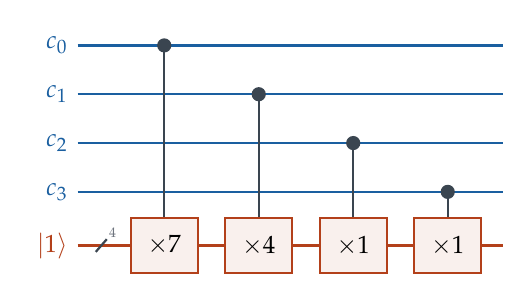
\begin{tikzpicture}[x=10mm,y=6.2mm]
        \foreach \j in {0,...,3} {
          \pgfmathsetmacro{\yy}{4-\j}
          \node[lab,color=cblue] at (0,\yy) {$c_{\j}$};
          \draw[cwire] (0,\yy) -- (5.4,\yy);}
        \node[lab,color=cverm] at (0,-0.1) {$|1\rangle$}; \draw[twire] (0,-0.1) -- (5.4,-0.1); \bundle{0.3}{-0.1}{$4$}
        \foreach \j/\c in {0/7,1/4,2/1,3/1} {
          \pgfmathsetmacro{\xx}{1.1+\j*1.2}
          \pgfmathsetmacro{\yy}{4-\j}
          \draw[thick,color=body] (\xx,\yy) -- (\xx,0.3); \node[dot] at (\xx,\yy) {};
          \node[op,minimum width=8.5mm,minimum height=7mm] at (\xx,-0.1) {$\times\c$};}
      \end{tikzpicture}\par
      {\small $N=15$, $a=7$: rungs $\times7,\times4,\times1,\times1$}
    \end{column}
    \begin{column}{0.48\textwidth}
      \begin{greyblock}
        Without it: $2^t-1$ applications of $U_a$ --- 15 instead of 4 at $t=4$, exponentially many at size.
      \end{greyblock}
      {\small At $N=15$ the rungs from the third on multiply by 1; a circuit compiled for 15 deletes them (7 NMR qubits, 2001).}
    \end{column}
  \end{columns}
  \code[basicstyle=\ttfamily\footnotesize]{ladder.py}
\end{frame}

\setcounter{framenumber}{41}
\begin{frame}{Free, before anything else: control only what does not cancel}
  Control only some gates of $V=G_L\cdots G_1$: with the control off, the rest still runs. So
  \[ \text{C-}V\ \text{needs a control on } G_j \text{ only if the uncontrolled residue would not cancel.} \]
  \vskip-1mm
  \begin{columns}[c]
    \begin{column}{0.53\textwidth}
      \centering
      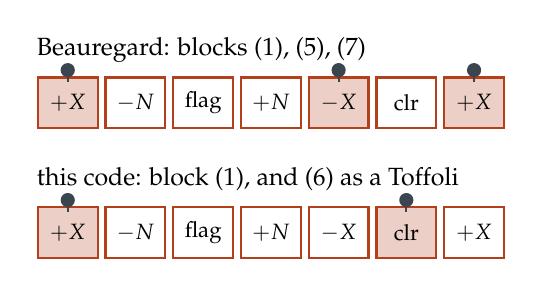
\begin{tikzpicture}[x=8.6mm,y=7.5mm,blk/.style={draw=cverm,thick,minimum width=7.6mm,minimum height=6.4mm,font=\footnotesize,inner sep=0pt,fill=white},
          on/.style={fill=cverm!25}]
        \node[font=\small,anchor=west] at (0.4,3.1) {Beauregard: blocks (1), (5), (7)};
        \foreach \i/\l in {1/{$+X$},2/{$-N$},3/{flag},4/{$+N$},5/{$-X$},6/{clr},7/{$+X$}}
          \node[blk] at (\i,2.2) {\l};
        \foreach \i/\l in {1/{$+X$},5/{$-X$},7/{$+X$}} {
          \node[blk,on] at (\i,2.2) {\l}; \draw[thick,color=body] (\i,2.55) -- (\i,2.75); \node[dot] at (\i,2.75) {};}
        \node[font=\small,anchor=west] at (0.4,0.9) {this code: block (1), and (6) as a Toffoli};
        \foreach \i/\l in {1/{$+X$},2/{$-N$},3/{flag},4/{$+N$},5/{$-X$},6/{clr},7/{$+X$}}
          \node[blk] at (\i,0) {\l};
        \foreach \i/\l in {1/{$+X$},6/{clr}} {
          \node[blk,on] at (\i,0) {\l}; \draw[thick,color=body] (\i,0.35) -- (\i,0.55); \node[dot] at (\i,0.55) {};}
      \end{tikzpicture}
    \end{column}
    \begin{column}{0.43\textwidth}
      \small
      \textbf{Conjugation:} in $ABA^\dagger$ control $B$ only --- Draper's adder controls its phases, not its QFTs.\par\vskip1mm
      \textbf{Compensating residue:} with the control off, blocks (2)--(4) and (6) cancel each other, because $y<N$.
    \end{column}
  \end{columns}
  \begin{peachblock}\peachtitle{Measured, $N=15$, $a=7$ (CNOTs / depth)}
    modular adder $2\,634\,/\,4\,836\to\mathbf{206\,/\,354}$ ($12.8\times$); \quad whole C-$U_a$ $20\,892\,/\,37\,727\to\mathbf{1\,748\,/\,2\,957}$ ($12.0\times$)
  \end{peachblock}
\end{frame}

\setcounter{framenumber}{43}
\begin{frame}{In Qiskit: a dynamic circuit}
  \centering\fig[width=0.96\textwidth]{semiclassical_phase.pdf}\par
  {\footnotesize\color{subtle}The loop on its own, with phase gates as the rungs ($y=5$, $t=3$): Aer reads back \texttt{101} on every shot.}
  \vskip1mm
  \raggedright
  \texttt{if\_test}: \textbf{mid-circuit measurement and feed-forward}.
\end{frame}

\setcounter{framenumber}{44}
\begin{frame}[fragile]{The loop in code}
  \code[basicstyle=\ttfamily\scriptsize]{semiclassical.py}
  \begin{columns}[T]
    \begin{column}{0.47\textwidth}
      \blocktitle{One loop, both problems}
      The rungs are callbacks: the same function drives factoring and ECDLP.
    \end{column}
    \begin{column}{0.47\textwidth}
      \blocktitle{Checked exactly}
      Enumerating the measurement branches, its distribution equals the full circuit's to $10^{-13}$.
    \end{column}
  \end{columns}
\end{frame}

\setcounter{framenumber}{45}
\begin{frame}{$N=21$ on 13 qubits instead of 22}
  \centering\fig[width=0.97\textwidth]{n21_measured.pdf}\par
  {\scriptsize\color{subtle}bars: Aer, 1024 shots of the one-counting-qubit circuit; dots: the exact distribution around each peak $s\cdot2^{10}/6$.}
  \vskip2mm
  \begin{columns}[T]
    \begin{column}{0.47\textwidth}
      \blocktitle{Same distribution}
      total variation distance $0.075$, within the shot-noise bound $0.108$.
    \end{column}
    \begin{column}{0.47\textwidth}
      \blocktitle{Same success}
      one shot gives $r=6$ with probability $0.322$ exact, $0.313$ measured; $21=7\times3$.
    \end{column}
  \end{columns}
\end{frame}

\setcounter{framenumber}{47}
\begin{frame}[fragile]{Controlling the ripple-carry adder: two gates of six}
  \begin{columns}[c]
    \begin{column}{0.55\textwidth}
      \centering
      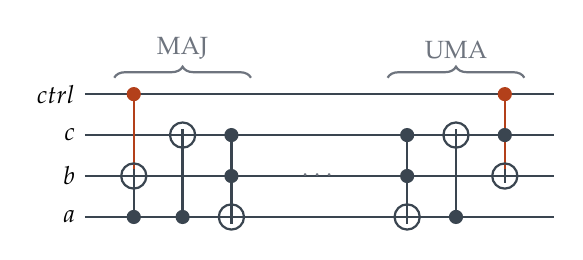
\begin{tikzpicture}[x=6.2mm,y=5.2mm]
        \foreach \y/\l in {3/ctrl,2/c,1/b,0/a} {\node[lab] at (0,\y) {$\l$}; \draw[wire] (0,\y) -- (9.6,\y);}
        \draw[thick,color=cverm] (1,3) -- (1,1); \node[dot,fill=cverm] at (1,3) {}; \node[dot] at (1,0) {}; \draw[thick,color=body] (1,0) -- (1,1); \oplusat{1}{1}
        \draw[thick,color=body] (2,0) -- (2,2); \node[dot] at (2,0) {}; \oplusat{2}{2}
        \draw[thick,color=body] (3,2) -- (3,0); \node[dot] at (3,2) {}; \node[dot] at (3,1) {}; \oplusat{3}{0}
        \draw[thick,color=body] (6.6,2) -- (6.6,0); \node[dot] at (6.6,2) {}; \node[dot] at (6.6,1) {}; \oplusat{6.6}{0}
        \draw[thick,color=body] (7.6,0) -- (7.6,2); \node[dot] at (7.6,0) {}; \oplusat{7.6}{2}
        \draw[thick,color=cverm] (8.6,3) -- (8.6,1); \node[dot,fill=cverm] at (8.6,3) {}; \node[dot] at (8.6,2) {}; \oplusat{8.6}{1}
        \draw[decorate,decoration={brace,amplitude=4pt},thick,color=subtle] (0.6,3.4) -- (3.4,3.4) node[midway,above=3pt,font=\small] {MAJ};
        \draw[decorate,decoration={brace,amplitude=4pt},thick,color=subtle] (6.2,3.4) -- (9.0,3.4) node[midway,above=3pt,font=\small] {UMA};
        \node[font=\small,color=subtle] at (4.8,1) {$\cdots$};
      \end{tikzpicture}
    \end{column}
    \begin{column}{0.41\textwidth}
      \small Only the two CNOTs into $b$ (\tgt{vermillion}) take the outer control. With it off, MAJ leaves two gates and UMA the same two reversed, so the chains cancel from the inside out.\par\vskip1mm
      {\color{cverm}\bfseries $2n$ controlled gates, not $6n$.}
    \end{column}
  \end{columns}
  \code[basicstyle=\ttfamily\scriptsize]{rc_majuma.py}
\end{frame}

\setcounter{framenumber}{48}
\begin{frame}{Ripple-carry against Fourier, measured}
  \begin{columns}[T]
    \begin{column}{0.56\textwidth}
      \centering\footnotesize
      \renewcommand{\arraystretch}{1.12}
      \begin{tabular}{@{}llrrrr@{}}
        \toprule
        adder & & qubits & rot. & Toffoli & depth \\
        \midrule
        $N=15$ & Fourier & 7 & 125 & 0 & 492 \\
        & ripple-carry & 13 & \textbf{0} & 71 & 578 \\
        \midrule
        $N=63$ & Fourier & 9 & 245 & 0 & 948 \\
        & ripple-carry & 17 & \textbf{0} & 99 & \textbf{844} \\
        \bottomrule
      \end{tabular}\par
      \vskip2mm
      \raggedright{\small One modular adder. Rotations grow as $n^2$ ($125\to245$), Toffolis as $n$ ($71\to99$); from $n=6$ ripple-carry is shallower too.}
    \end{column}
    \begin{column}{0.4\textwidth}
      \begin{greyblock}[fontupper=\small]
        \blocktitle{Which to use}
        \emph{Simulating} small $N$: Fourier --- $4n+2$ qubits against $5n+4$ is the whole cost of a statevector.\par\vskip1mm
        \emph{Fault tolerance}: ripple-carry. No rotations, and the T count is the bill.
      \end{greyblock}
    \end{column}
  \end{columns}
  \begin{takeaway}The smallest Fourier rotation is $2\pi/2^{n+1}$: $10^{-616}$ rad at $n=2048$. At size, Fourier arithmetic must be approximated before it can be run at all.\end{takeaway}
\end{frame}

\setcounter{framenumber}{49}
\begin{frame}{Toffolis are cheaper than rotations}
  \begin{columns}[c]
    \begin{column}{0.52\textwidth}
      \centering\fig[width=\textwidth]{rung_T.pdf}
    \end{column}
    \begin{column}{0.44\textwidth}
      One rung, T gates with every rotation synthesised.
      \vskip2mm
      \begin{greyblock}
        Ripple-carry: 7--8$\times$ \textbf{more} Toffolis, but no rotations.\par
        T: $\div19$ at $n=4$, $\div99$ at $n=12$.
      \end{greyblock}
      {\small The gap grows like $n$: rotations scale as $n^4$, Toffolis as $n^3$.}
    \end{column}
  \end{columns}
\end{frame}

\setcounter{framenumber}{51}
\begin{frame}[fragile]{The temporary AND, in code}
  \begin{columns}[T]
    \begin{column}{0.33\textwidth}
      \code[basicstyle=\ttfamily\scriptsize]{and_compute.py}
    \end{column}
    \begin{column}{0.63\textwidth}
      \centering\footnotesize
      \renewcommand{\arraystretch}{1.1}
      \begin{tabular}{@{}rrrrr@{}}
        \toprule
        bits & $L$ & T (Toffolis) & T (temp.\ ANDs) & saving \\
        \midrule
        2 & 4 & 42 & 12 & $3.50\times$ \\
        3 & 8 & 98 & 28 & $3.50\times$ \\
        4 & 16 & 210 & 60 & $3.50\times$ \\
        5 & 32 & 434 & 124 & $3.50\times$ \\
        \bottomrule
      \end{tabular}\par
      {\scriptsize one unary-iteration lookup, transpiled to Clifford$+$T}\par
      \vskip1.5mm
      \raggedright\small
      Exactly $7/2$: half the Toffolis were uncomputes, now free; the rest fell from 7 T to 4. The last gate is $S^\dagger$: three plausible variants differ only there, and all are wrong.
    \end{column}
  \end{columns}
  \code[basicstyle=\ttfamily\scriptsize]{and_uncompute.py}
\end{frame}

\setcounter{framenumber}{53}
\begin{frame}[fragile]{Windowing: look the answer up, then add once}
  \begin{columns}[c]
    \begin{column}{0.62\textwidth}
      \centering
      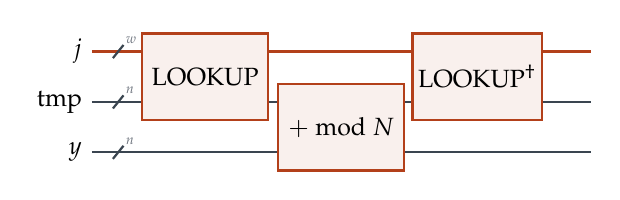
\begin{tikzpicture}[x=9.6mm,y=6.4mm]
        \node[lab] at (0,2) {$j$}; \draw[twire] (0,2) -- (6.6,2); \bundle{0.35}{2}{$w$}
        \node[lab] at (0,1) {tmp}; \draw[wire] (0,1) -- (6.6,1); \bundle{0.35}{1}{$n$}
        \node[lab] at (0,0) {$y$}; \draw[wire] (0,0) -- (6.6,0); \bundle{0.35}{0}{$n$}
        \node[op,minimum width=16mm,minimum height=11mm] at (1.5,1.5) {LOOKUP};
        \node[op,minimum width=16mm,minimum height=11mm] at (3.3,0.5) {$+$ mod $N$};
        \node[op,minimum width=16mm,minimum height=11mm] at (5.1,1.5) {LOOKUP$^\dagger$};
      \end{tikzpicture}
    \end{column}
    \begin{column}{0.34\textwidth}
      \small tmp $\leftarrow T[j]$; \ $y\leftarrow y+\text{tmp}$; \ tmp $\leftarrow0$.\par\vskip1mm
      The addend is now \emph{quantum}: Draper's phase ramp takes its rotations from the bits of tmp; the seven blocks are unchanged.
    \end{column}
  \end{columns}
  \code[basicstyle=\ttfamily\scriptsize]{add_quantum_mod.py}
\end{frame}

\setcounter{framenumber}{54}
\begin{frame}[fragile]{Windowing, in code}
  \code[basicstyle=\ttfamily\scriptsize]{windowed.py}
  \begin{columns}[T]
    \begin{column}{0.5\textwidth}
      \begin{greyblock}[fontupper=\small]
        \blocktitle{Why $c=0$ entries of 0 are the trick}
        With $c=0$ the lookup writes 0, and the seven blocks with $t=0$ undo themselves: no controlled gate in the adder.
      \end{greyblock}
    \end{column}
    \begin{column}{0.44\textwidth}
      \small The second \texttt{lookup\_ui} uncomputes the first --- a cost the next slides remove.
    \end{column}
  \end{columns}
\end{frame}

\setcounter{framenumber}{55}
\begin{frame}{Windowing, measured}
  \begin{columns}[T]
    \begin{column}{0.55\textwidth}
      \centering\footnotesize
      \renewcommand{\arraystretch}{1.08}
      \begin{tabular}{@{}lrrrr@{}}
        \toprule
        $y\mathrel{+}=kx$, $N=255$ & adds & qubits & CNOT & depth \\
        \midrule
        shift-and-add & 8 & 19 & 7\,390 & 13\,020 \\
        window $w=2$ & 4 & 29 & 4\,840 & 6\,497 \\
        window $w=3$ & 3 & 30 & 3\,902 & 4\,873 \\
        window $w=4$ & 2 & 31 & \textbf{3\,264} & \textbf{3\,866} \\
        \bottomrule
      \end{tabular}\par
      \vskip3mm
      \begin{tabular}{@{}lrrr@{}}
        \toprule
        full circuit, $N=15$ & qubits & CNOT & depth \\
        \midrule
        plain, $t=8$ & 18 & 20\,462 & 34\,537 \\
        windowed $w=2$, $t=8$ & 24 & 14\,276 & \textbf{17\,028} \\
        \bottomrule
      \end{tabular}
    \end{column}
    \begin{column}{0.41\textwidth}
      \small
      \blocktitle{Depth falls faster than additions}
      Lookups are shallow; the additions they replace were not. At $n=8$: CNOTs $\div2.3$, depth $\div3.4$, for 12 more qubits.
      \vskip1.5mm
      \blocktitle{End to end on Aer}
      $N=15$, $t=8$, 24 qubits: all 2\,048 shots on the four peaks.\par
      $N=21$, $t=10$, 29 qubits (68 min): the six peaks, $r=6$, $21=7\times3$.
    \end{column}
  \end{columns}
\end{frame}

\setcounter{framenumber}{57}
\begin{frame}[fragile]{Unary iteration, in code: $m$ ancillas, the control at the root}
  \code[basicstyle=\ttfamily\fontsize{7.6}{8.8}\selectfont]{lookup_ui.py}
\end{frame}

\setcounter{framenumber}{59}
\begin{frame}[fragile]{Measured uncomputation, in code: the controller sits in the middle}
  \code[basicstyle=\ttfamily\footnotesize]{phase_fixup.py}
  \begin{columns}[T]
    \begin{column}{0.47\textwidth}
      \blocktitle{Not one static circuit}
      $F$ depends on the outcome, so it runs as circuit $\to$ measure $\to$ classical $\to$ circuit, as on hardware (\texttt{run\_windowed\_acc\_mbu}).
    \end{column}
    \begin{column}{0.47\textwidth}
      \blocktitle{Checked}
      Exactly $\mathrm{diag}((-1)^{F[a]})$ for every split; in the windowed accumulate, 180 mid-circuit measurements leave every register exact.
    \end{column}
  \end{columns}
\end{frame}

\setcounter{framenumber}{60}
\begin{frame}{Nested windows: window the exponent too}
  \begin{columns}[c]
    \begin{column}{0.5\textwidth}
      \centering
      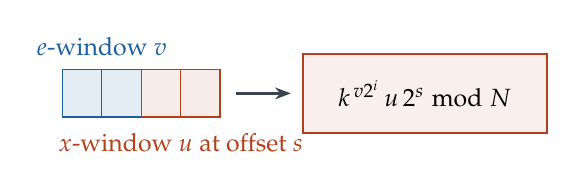
\begin{tikzpicture}[x=5mm,y=6mm]
        \foreach \i in {0,1} \draw[draw=cblue,fill=cblue!12] (\i,0) rectangle (\i+1,1);
        \foreach \i in {2,3} \draw[draw=cverm,fill=cverm!10] (\i,0) rectangle (\i+1,1);
        \node[font=\small,color=cblue] at (1,1.5) {$e$-window $v$};
        \node[font=\small,color=cverm] at (3,-0.55) {$x$-window $u$ at offset $s$};
        \draw[-{Stealth[length=2mm]},thick,color=body] (4.4,0.5) -- (5.8,0.5);
        \node[op,minimum width=31mm,minimum height=10mm,font=\small] at (9.2,0.5) {$k^{\,v2^i}\,u\,2^{s}\bmod N$};
      \end{tikzpicture}
      \vskip3mm
      \raggedright\small
      \begin{itemize}\setlength{\itemsep}{0.6mm}
        \item $\lceil t/w_e\rceil$ multiplications instead of $t$;
        \item \textbf{no control}: window 0 selects $k^0=1$;
        \item the swap becomes a \textbf{relabelling}: no Fredkins.
      \end{itemize}
    \end{column}
    \begin{column}{0.46\textwidth}
      \centering\footnotesize
      \renewcommand{\arraystretch}{1.1}
      \begin{tabular}{@{}lrrr@{}}
        \toprule
        $N=15$, $t=8$ & mults & CNOT & depth \\
        \midrule
        plain & 8 & 20\,462 & 34\,537 \\
        windowed $w_m=2$ & 8 & 14\,276 & 17\,028 \\
        nested $w_e=2$ & 4 & \textbf{11\,908} & \textbf{14\,229} \\
        nested $w_e=4$ & 2 & 16\,292 & 20\,095 \\
        \bottomrule
      \end{tabular}\par
      \vskip2mm
      \begin{peachblock}[fontupper=\small]\peachtitle{Windows have an optimum}
        At $w_e=4$ the $2^6$-entry table costs more than the two multiplications it saves.
      \end{peachblock}
    \end{column}
  \end{columns}
\end{frame}

\setcounter{framenumber}{61}
\begin{frame}[fragile]{Nested windows, in code}
  \code[basicstyle=\ttfamily\fontsize{7.6}{8.8}\selectfont]{nested.py}
  \begin{columns}[T]
    \begin{column}{0.47\textwidth}
      {\small\textbf{Checked:} $|e\rangle|1\rangle|0\rangle\mapsto|e\rangle|7^e\bmod15\rangle|0\rangle$ for all $e<16$; factors 15 on 23 qubits, 2 multiplications.}
    \end{column}
    \begin{column}{0.47\textwidth}
      {\small\textbf{Not with one counting qubit:} $w_e$ exponent bits must coexist as an address; the two are ends of one spectrum.}
    \end{column}
  \end{columns}
\end{frame}

\setcounter{framenumber}{62}
\begin{frame}[fragile]{Coset representation: delete the modular reduction}
  Store $k$ as a comb over $c$ padding qubits (Zalka; Gidney--Ekerå):\par
  {\centering $|k\rangle_{\mathrm{coset}}=2^{-c/2}\sum_{j<2^c}|jN+k\rangle$\par}
  \begin{columns}[c]
    \begin{column}{0.55\textwidth}
      \centering
      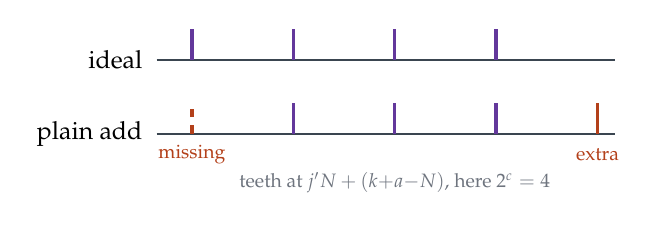
\begin{tikzpicture}[x=5.6mm,y=5.2mm]
        \draw[thick,color=body] (0,1.8) -- (10.4,1.8); \draw[thick,color=body] (0,0) -- (10.4,0);
        \node[font=\small,anchor=east] at (-0.1,1.8) {ideal}; \node[font=\small,anchor=east] at (-0.1,0) {plain add};
        \foreach \j in {0,...,3} {\draw[very thick,color=cpurple] (0.8+\j*2.3,1.8) -- (0.8+\j*2.3,2.55);}
        \foreach \j in {1,...,3} {\draw[very thick,color=cpurple] (0.8+\j*2.3,0) -- (0.8+\j*2.3,0.75);}
        \draw[very thick,color=cverm] (0.8+4*2.3,0) -- (0.8+4*2.3,0.75);
        \draw[very thick,color=cverm,dashed] (0.8,0) -- (0.8,0.75);
        \node[font=\scriptsize,color=cverm] at (10.0,-0.5) {extra}; \node[font=\scriptsize,color=cverm] at (0.8,-0.5) {missing};
        \node[font=\scriptsize,color=subtle] at (5.4,-1.2) {teeth at $j'N+(k{+}a{-}N)$, here $2^c=4$};
      \end{tikzpicture}
    \end{column}
    \begin{column}{0.41\textwidth}
      \small Every branch is $\equiv k\pmod N$, so a \textbf{plain} addition of $a$ gives branches $\equiv k+a$. When $k+a\ge N$ the comb re-indexes, and differs from the ideal state in \textbf{two edge teeth} out of $2^c$. That is the entire approximation.
    \end{column}
  \end{columns}
  \begin{columns}[c]
    \begin{column}{0.47\textwidth}
      \code[basicstyle=\ttfamily\footnotesize]{coset_add.py}
    \end{column}
    \begin{column}{0.49\textwidth}
      \begin{peachblock}\peachtitle{One addition, coset vs seven blocks}
        Fourier: $1.7\times$ ($N=15$) to $2.8\times$ ($N=1023$) fewer CNOTs. Ripple-carry: $3.0\times$ to $3.9\times$ fewer Toffolis.
      \end{peachblock}
    \end{column}
  \end{columns}
\end{frame}

\setcounter{framenumber}{63}
\begin{frame}{Coset representation, measured}
  \begin{columns}[T]
    \begin{column}{0.46\textwidth}
      \centering\footnotesize
      \renewcommand{\arraystretch}{1.04}
      \begin{tabular}{@{}rrrr@{}}
        \toprule
        $N$ & $c$ & error, 8 adds & bound $8/2^c$ \\
        \midrule
        15 & 2 & 0.749 & 2.000 \\
           & 3 & 0.373 & 1.000 \\
           & 4 & 0.129 & 0.500 \\
           & 5 & 0.031 & 0.250 \\
           & 6 & 0.000 & 0.125 \\
        \midrule
        31 & 2 & 0.507 & 2.000 \\
           & 4 & 0.061 & 0.500 \\
        \bottomrule
      \end{tabular}\par
      {\scriptsize The error halves per padding qubit. Approximate by design: the tests measure a rate, not equality.}
    \end{column}
    \begin{column}{0.5\textwidth}
      \begin{peachblock}[fontupper=\small]\peachtitle{A friendly modulus hides the effect}
        At $N=21$ the error was 0 for every $c$: $2^n-N=11$ leaves so much headroom that no branch wraps. Hence 15 and 31, just below $2^n$.
      \end{peachblock}
      \small
      \blocktitle{Multiplying works too}
      Branch bits differ, yet $\sum_iv_i(A2^i\bmod N)\equiv A(jN+x)\equiv Ax$. At $N=7$, $c=4$: worst error $0.0135$.\par
      \vskip1mm
      The coset order-finding circuit (\texttt{coset.order\_circuit\_coset}) is checked at $N=15$.
    \end{column}
  \end{columns}
\end{frame}

\setcounter{framenumber}{64}
\begin{frame}{Approximate QFT: fewer rotations, but errors add up}
  Drop every $\mathrm{CP}(\pi/2^k)$ with $k>d$, in every adder's QFT. On $N=15$:
  \vskip2mm
  \centering
  \renewcommand{\arraystretch}{1.2}
  \begin{tabular}{lrrr}
    \toprule
    QFTs & small rotations & distance from exact & P(one shot gives $r$) \\
    \midrule
    exact & 12\,855 & 0.006 & 0.501 \\
    $d=4$ & 12\,837 & 0.006 & 0.501 \\
    $d=3$ & 10\,905 & \textbf{0.138} & 0.451 \\
    $d=2$ & 7\,050 & \textbf{0.594} & 0.245 \\
    \bottomrule
  \end{tabular}
  \vskip2mm
  \raggedright{\small 320 Fourier additions, each with its own approximation error: they accumulate. Shot-noise bound: 0.032.}
  \begin{takeaway}One error budget is shared by every approximation, so $d$ must grow like $\log_2(\#\text{additions}/\varepsilon)$. At $n=8$, $d=4$ already removes a third of the rotations.\end{takeaway}
\end{frame}

\setcounter{framenumber}{65}
\begin{frame}{Act VII in plain words (1/2)}
  \centering\footnotesize
  \renewcommand{\arraystretch}{1.15}
  \begin{tabular}{@{}>{\raggedright}p{30mm}>{\raggedright}p{63mm}>{\raggedright\arraybackslash\leavevmode\color{cverm}}p{40mm}@{}}
    \toprule
    optimisation & what it does & \color{ink}what it bought \\
    \midrule
    \textbf{Precomputed powers} & $U_a^{2^j}$ is one multiplication by the constant $a^{2^j}\bmod N$, squared on a laptop & $t$ rungs instead of $2^t-1$ multiplications \\
    \textbf{Control placement} & of the seven blocks of a controlled adder, only those that do not cancel need the control & $12.8\times$ fewer CNOTs per adder ($N=15$) \\
    \textbf{Semiclassical QFT} & measure each counting qubit first, apply the rotations classically, reuse one qubit & $4n+2\to2n+3$ qubits; $N=21$ on 13 \\
    \textbf{Ripple-carry adder} & add with Toffolis and CNOTs, no small rotations & T $\div19$ ($n=4$) to $\div99$ ($n=12$) \\
    \textbf{Controlled MAJ/UMA} & control only the two CNOTs per bit that write the target & $2n$ controlled gates, not $6n$ \\
    \textbf{Temporary AND} & a Toffoli onto $|0\rangle$ costs 4 T; undo it by an $X$ measurement and a classically controlled CZ & 14 T $\to$ 4 per pair; lookups $3.5\times$ cheaper \\
    \bottomrule
  \end{tabular}
\end{frame}

\setcounter{framenumber}{66}
\begin{frame}{Act VII in plain words (2/2)}
  \centering\footnotesize
  \renewcommand{\arraystretch}{1.15}
  \begin{tabular}{@{}>{\raggedright}p{30mm}>{\raggedright}p{63mm}>{\raggedright\arraybackslash\leavevmode\color{cverm}}p{40mm}@{}}
    \toprule
    optimisation & what it does & \color{ink}what it bought \\
    \midrule
    \textbf{Windowing} & take $w$ bits at once, look up their contribution, add once; the control becomes one more address bit & $n\to\lceil n/w\rceil$ additions; one rung $4.0\to1.2$M T \\
    \textbf{Unary iteration} & walk the table's addresses with a tree of ANDs on about $w$ ancillas & $59\to31$ qubits ($n=8$, $w=4$) \\
    \textbf{Measured uncomputation} & erase a lookup by an $X$ measurement and an $O(\sqrt L)$ phase repair, not a second lookup & $4\,094\to157$ Toffolis at $w=11$ \\
    \textbf{Nested windows} & window the exponent too: one multiplication covers several exponent bits & $8\to4$ multiplications ($N=15$) \\
    \textbf{Coset representation} & store $k$ as $\sum_j|jN+k\rangle$; a plain adder then adds mod $N$, error $\approx2^{-c}$ & $3.0$--$3.9\times$ fewer Toffolis per addition \\
    \textbf{Approximate QFT} & drop the rotations finer than $\pi/2^d$ & $-34\%$ rotations; errors add up \\
    \bottomrule
  \end{tabular}
\end{frame}

\setcounter{framenumber}{67}
\begin{frame}{All together: $N=15$}
  \centering\fig[width=0.96\textwidth]{variants.pdf}
  \vskip1mm
  \raggedright
  {\small Priced with synthesis, ripple-carry wins by $20\times$: 17 qubits and 42\,600 T, against 18 and 978\,000.}
  \resolved{Remove rotations first, then qubits, then additions.}
\end{frame}

% ======================================================================
\act{Optimisations in detail --- elliptic curves, toy size (Act VIII)}

\setcounter{framenumber}{79}
\begin{frame}{L0: temporary ANDs --- and which Toffolis are counted}
  \begin{columns}[T]
    \begin{column}{0.52\textwidth}
      \centering\footnotesize
      \renewcommand{\arraystretch}{1.12}
      \begin{tabular}{@{}rrrrr@{}}
        \toprule
        $n$ & ANDs & AND$^\dagger$s & T (Toffoli) & T (AND) \\
        \midrule
        5 & 912 & 892 & 14\,938 & 5\,958 \\
        8 & 2\,229 & 2\,197 & 36\,694 & 14\,628 \\
        12 & 4\,785 & 4\,737 & 79\,254 & \textbf{31\,740} \\
        \bottomrule
      \end{tabular}\par
      {\scriptsize one modular inversion}\par
      \vskip2mm
      \raggedright\small
      A flat $2.50\times$: ANDs and AND$^\dagger$s come in equal numbers, so the average is $(4+0)/2=2$ T against 7 --- $3.5\times$, diluted by the Fredkins and dirty-target Toffolis that cannot use the trick.
    \end{column}
    \begin{column}{0.44\textwidth}
      \begin{greyblock}[fontupper=\small]
        \blocktitle{What counts as a Toffoli}
        Both papers count CCX, CCZ and AND gates; a measured AND$^\dagger$ has no T and is free. Counting every three-qubit operation instead nearly doubles Gidney-style circuits.\par\vskip1mm
        \texttt{ec\_cost} reports both (\texttt{toffoli\_paper}, \texttt{toffoli\_equiv}). Quoting the wrong one halves every optimisation here.
      \end{greyblock}
    \end{column}
  \end{columns}
\end{frame}

\setcounter{framenumber}{80}
\begin{frame}{L1: which adder, and how to control it}
  \centering\footnotesize
  \renewcommand{\arraystretch}{1.12}
  \begin{tabular}{@{}rrrrrr@{}}
    \toprule
    & \multicolumn{2}{c}{add} & \multicolumn{3}{c}{controlled add} \\
    \cmidrule(lr){2-3}\cmidrule(l){4-6}
    $n$ & CDKM & Gidney & promote & copy, CDKM & copy, Gidney \\
    \midrule
    8 & 16 & 7 & 32 & 24 & 15 \\
    16 & 32 & 15 & 64 & 48 & 31 \\
    32 & 64 & 31 & 128 & 96 & \textbf{63} \\
    \bottomrule
  \end{tabular}\par
  {\scriptsize Toffolis; ``promote'': every CNOT of the adder becomes a Toffoli}\par
  \vskip3mm
  \raggedright
  \begin{columns}[T]
    \begin{column}{0.48\textwidth}
      \small \textbf{CDKM}: $2n$ Toffolis on $2n+1$ qubits.\par\vskip1mm
      \textbf{Gidney}: $n-1$ ANDs on clean targets, free to uncompute (measure and fix the phase), on $3n-1$ qubits.
    \end{column}
    \begin{column}{0.48\textwidth}
      \small \textbf{Copy-then-add}: AND the addend into a clean register under the control, add unconditionally, un-AND. $2.0\times$ fewer Toffolis than promoting, of which $1.33\times$ is the control style alone.
    \end{column}
  \end{columns}
\end{frame}

\setcounter{framenumber}{81}
\begin{frame}[fragile]{Copy-then-add, in circuit and in code}
  \begin{columns}[c]
    \begin{column}{0.4\textwidth}
      \centering
      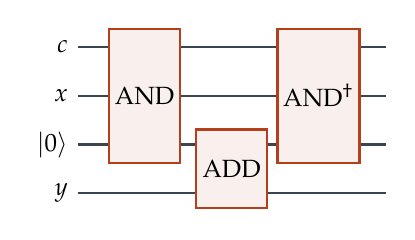
\begin{tikzpicture}[x=8.5mm,y=6.2mm]
        \foreach \y/\l in {3/{$c$},2/{$x$},1/{$|0\rangle$},0/{$y$}} {\node[lab] at (0,\y) {\l}; \draw[wire] (0,\y) -- (4.6,\y);}
        \node[op,minimum width=9mm,minimum height=17mm] at (1,2) {AND};
        \node[op,minimum width=9mm,minimum height=10mm] at (2.3,0.5) {ADD};
        \node[op,minimum width=9mm,minimum height=17mm] at (3.6,2) {AND$^\dagger$};
      \end{tikzpicture}\par
      \vskip1mm
      {\scriptsize $y\mathrel{+}=c\cdot x$; the copy is $|0\rangle$ again}
    \end{column}
    \begin{column}{0.56\textwidth}
      \code[basicstyle=\ttfamily\scriptsize]{cadd.py}
    \end{column}
  \end{columns}
  \vskip3mm
  {\small Only the copy sees the control: $n$ ANDs in, $n$ free AND$^\dagger$s out, and the adder in the middle is the cheap uncontrolled one. The same pattern controls every adder in the ECDLP circuit.}
\end{frame}

\setcounter{framenumber}{82}
\begin{frame}{L2: approximate and pseudo-Mersenne reduction}
  \begin{columns}[T]
    \begin{column}{0.5\textwidth}
      \small
      \blocktitle{Compare only the top bits}
      ``At least $p$?'' is right unless the top bits tie, probability $\approx2^{-\text{msbs}}$, and the flag comes \emph{before} the subtraction: one controlled subtraction instead of two steps.
      \vskip2mm
      \blocktitle{Use the shape of the prime}
      secp256k1: $p=2^{u}-f$, $f=2^{32}+977$. ``At least $p$?'' is almost ``bit $u$ set?'', and subtracting $p$ is ``clear bit $u$, add $f$'' --- on the low bits only.
    \end{column}
    \begin{column}{0.46\textwidth}
      \centering
      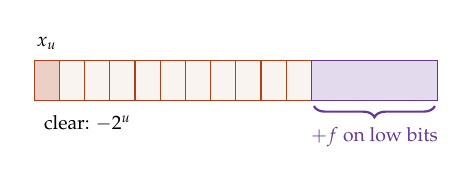
\begin{tikzpicture}[x=3.2mm,y=5mm]
        \draw[draw=cverm,fill=cverm!25] (0,0) rectangle (1,1); \node[font=\scriptsize] at (0.5,1.45) {$x_u$};
        \foreach \i in {1,...,15} \draw[draw=cverm,fill=cverm!6] (\i,0) rectangle (\i+1,1);
        \draw[draw=cpurple,fill=cpurple!18] (11,0) rectangle (16,1);
        \draw[decorate,decoration={brace,amplitude=4pt,mirror},thick,color=cpurple] (11.1,-0.15) -- (15.9,-0.15) node[midway,below=4pt,font=\scriptsize] {$+f$ on low bits};
        \node[font=\scriptsize,anchor=north west] at (0,-0.15) {clear: $-2^u$};
      \end{tikzpicture}
      \vskip2mm
      \footnotesize
      \renewcommand{\arraystretch}{1.08}
      \begin{tabular}{@{}lrrrr@{}}
        \toprule
        $p=4093$ & \multicolumn{2}{c}{doubling} & \multicolumn{2}{c}{ctrl.\ add} \\
        & Toff. & fail & Toff. & fail \\
        \midrule
        exact & 25 & 0\% & 73 & 0\% \\
        top 4 bits & 17 & 3.1\% & 51 & 9.7\% \\
        pseudo-M. & \textbf{4} & 3.1\% & 49 & 1.0\% \\
        \bottomrule
      \end{tabular}\par
      {\scriptsize Failures track $2^{-\text{msbs}}$: 8 bits give 0.17\%.}
    \end{column}
  \end{columns}
\end{frame}

\setcounter{framenumber}{83}
\begin{frame}[fragile]{Pseudo-Mersenne doubling, in code --- and why failures compound}
  \code[basicstyle=\ttfamily\fontsize{7.6}{8.8}\selectfont]{moddbl_pm.py}
  \begin{columns}[T]
    \begin{column}{0.48\textwidth}
      {\small Nothing compares anything: clearing the overflow bit \emph{is} the subtraction of $2^u$. A 2-bit comparison failing 12\% per step makes a whole multiplier fail 81\% ($p=31$): hence 40--50 bits at $n=256$.}
    \end{column}
    \begin{column}{0.48\textwidth}
      {\small \textbf{One case is not rare:} Alg.~10 cannot reduce $x+y=p$, and every multiplication meets it once. Alg.~11 catches it, with its flag test gated on the control.}
    \end{column}
  \end{columns}
\end{frame}

\setcounter{framenumber}{84}
\begin{frame}{L3: Montgomery multiplication over a carry-save tree}
  \begin{columns}[T]
    \begin{column}{0.45\textwidth}
      \small
      [106] rewrites the reduction $c\mathrel{+}=Mp$ as $c\mathrel{+}=c_w\cdot d$ with a \textbf{compile-time} $d=(p'_w\bmod 2^w)\,p$: the shape of the multiplication step, so one carry-save tree serves both.
      \vskip2mm
      A 3:2 compressor makes three addends two, $A+B+C=S+2M$, with one AND per bit and no carry chain: $O(\log w)$ depth.
      \vskip2mm
      \textbf{A depth optimisation}: $\div2.0$ at $n=16$, for $4\times$ the qubits; it does not beat the QROM multiplier on gates.
    \end{column}
    \begin{column}{0.51\textwidth}
      \centering
      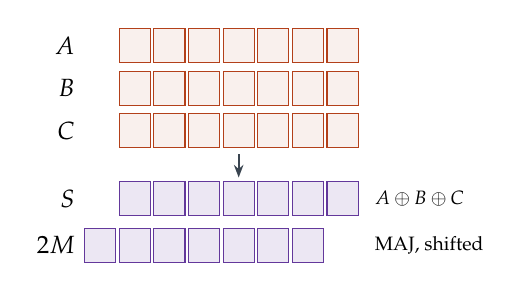
\begin{tikzpicture}[x=4.4mm,y=5.4mm]
        \foreach \r/\l/\c in {3/A/cverm,2/B/cverm,1/C/cverm} {
          \node[lab] at (-1,\r) {$\l$};
          \foreach \i in {0,...,6} \draw[draw=\c,fill=\c!8] (\i,\r-0.4) rectangle (\i+0.9,\r+0.4);}
        \draw[-{Stealth[length=1.6mm]},thick,color=body] (3.45,0.45) -- (3.45,-0.1);
        \node[lab] at (-1,-0.6) {$S$}; \foreach \i in {0,...,6} \draw[draw=cpurple,fill=cpurple!12] (\i,-1) rectangle (\i+0.9,-0.2);
        \node[lab] at (-1,-1.7) {$2M$}; \foreach \i in {-1,...,5} \draw[draw=cpurple,fill=cpurple!12] (\i,-2.1) rectangle (\i+0.9,-1.3);
        \node[font=\scriptsize,anchor=west] at (7.1,-0.6) {$A\oplus B\oplus C$};
        \node[font=\scriptsize,anchor=west] at (7.1,-1.7) {MAJ, shifted};
      \end{tikzpicture}
      \vskip2mm
      \footnotesize
      \renewcommand{\arraystretch}{1.08}
      \begin{tabular}{@{}lrrr@{}}
        \toprule
        $n=16$, $w=4$ & Toffoli & qubits & depth \\
        \midrule
        schoolbook & 2\,080 & 86 & 13\,043 \\
        carry-save tree & 1\,566 & 324 & \textbf{6\,669} \\
        QROM lookup & 1\,054 & 347 & 4\,780 \\
        \bottomrule
      \end{tabular}
    \end{column}
  \end{columns}
\end{frame}

\setcounter{framenumber}{85}
\begin{frame}[fragile]{The 3:2 compressor, in code}
  \code[basicstyle=\ttfamily\fontsize{7.6}{8.8}\selectfont]{csa.py}
  {\small The rewritten reduction over-adds by up to $2^{2w}p$, so the accumulator settles at $n+2w$ bits, not Montgomery's $n+2$; the tests measure that width rather than trust it.}
\end{frame}

\setcounter{framenumber}{86}
\begin{frame}[fragile]{L3: Kaliski with every round run, and the reductions postponed}
  \begin{columns}[T]
    \begin{column}{0.54\textwidth}
      \small
      \textbf{Run every round.} An inert round only doubles $r$, so every input ends at $-x^{-1}2^{2n}$: no counter, no corrective halvings --- one negation instead.\par\vskip1mm
      \textbf{Reduce once, at the end.} With $r,s$ on $2n$ bits a modular doubling is a shift, i.e.\ a renaming of wires, and a modular addition a plain one.
    \end{column}
    \begin{column}{0.42\textwidth}
      \centering\footnotesize
      \renewcommand{\arraystretch}{1.08}
      \begin{tabular}{@{}rrrrr@{}}
        \toprule
        & \multicolumn{2}{c}{Toffoli} & \multicolumn{2}{c}{depth} \\
        $n$ & before & after & before & after \\
        \midrule
        5 & 1\,242 & 817 & 4\,846 & 2\,664 \\
        8 & 3\,045 & 2\,077 & 12\,271 & 7\,019 \\
        12 & 6\,585 & \textbf{4\,653} & 27\,239 & \textbf{16\,059} \\
        \bottomrule
      \end{tabular}\par
      {\scriptsize Häner et al.\ 2020 $\to$ [106], $+11\%$ qubits}
    \end{column}
  \end{columns}
  \code[basicstyle=\ttfamily\scriptsize]{kaliski_opt.py}
\end{frame}

\setcounter{framenumber}{87}
\begin{frame}{L3 rebuilt: the Euclidean dialog}
  \begin{columns}[T]
    \begin{column}{0.52\textwidth}
      Inversion and multiplication are \textbf{one job} ([1128], after Khattar et al.). Run the binary GCD on $(u,v)=(p,x)$ \emph{without} the Bézout coefficients; keep only two decision bits per round, the \textbf{dialog}:
      \vskip1mm
      \begin{greyblock}[fontupper=\small]
        repeat $\approx1.413n$ times:\\
        \quad $b_0:=v\bmod2$,\quad $b_1:=[u>v]$\\
        \quad record $b_0$ and $b_0b_1$\\
        \quad if $b_0b_1$: swap $u,v$\\
        \quad if $b_0$: $v\mathrel{-}=u$\\
        \quad $v\mathrel{/}=2$
      \end{greyblock}
    \end{column}
    \begin{column}{0.44\textwidth}
      \small
      \blocktitle{Why $1.413n$ rounds}
      Halving always removes a bit, the subtraction a second one half the time: $uv$ shrinks by $3/8$ per round, $2n/\log_2(8/3)\approx1.413n$. Measured: $1.383n$ at $n=32$, $1.409n$ at $n=256$; spread $\approx0.6\sqrt n$, hence the $+c\sqrt n$ margin.
      \vskip2mm
      \blocktitle{Packing the record}
      $(b_0,b_0b_1)$ is never $(0,1)$: three pairs have $27<32$ states, so they fit in 5 bits. Record $2.83n\to2.355n$, at a fixed size.
    \end{column}
  \end{columns}
\end{frame}

\setcounter{framenumber}{88}
\begin{frame}[fragile]{One round of the dialog, in code}
  \code[basicstyle=\ttfamily\fontsize{7.6}{8.8}\selectfont]{dialog_round.py}
\end{frame}

\setcounter{framenumber}{89}
\begin{frame}[fragile]{The replay: the same decisions, applied to any pair}
  \begin{columns}[T]
    \begin{column}{0.48\textwidth}
      \small The updates the full extended Euclid makes to $(r,s)$ are \textbf{linear} in the recorded bits, so they can be replayed afterwards onto any pair:
      \vskip1mm
      \centering$s\leftarrow2s;\quad \text{if } b_0:\ s\mathrel{+}=r;$\\[0.5mm]
      $\text{if } b_0b_1:\ \text{swap}(r,s).$
    \end{column}
    \begin{column}{0.48\textwidth}
      \begin{peachblock}[fontupper=\small]\peachtitle{Direction matters}
        Read backwards from $(y,0)$ the replay ends at $(0,\,xy\bmod p)$ and needs only doubling; forwards it divides, with halving. Run the circuit in reverse to divide.
      \end{peachblock}
    \end{column}
  \end{columns}
  \code[basicstyle=\ttfamily\scriptsize]{bezout_replay.py}
\end{frame}

\setcounter{framenumber}{90}
\begin{frame}[fragile]{In-place multiplication: dialog, replay, dialog backwards}
  \code[basicstyle=\ttfamily\fontsize{7.6}{8.8}\selectfont]{inplace_mul_short.py}
  \begin{columns}[T]
    \begin{column}{0.5\textwidth}
      \centering\footnotesize
      \renewcommand{\arraystretch}{1.08}
      \begin{tabular}{@{}rrrrr@{}}
        \toprule
        & \multicolumn{2}{c}{invert, then multiply} & \multicolumn{2}{c}{dialog $+$ replay} \\
        $p$ & Toffoli & qubits & Toffoli & qubits \\
        \midrule
        7 & 1\,095 & 64 & 612 & 39 \\
        31 & 2\,889 & 99 & 1\,378 & 57 \\
        61 & 4\,068 & 115 & \textbf{1\,875} & \textbf{66} \\
        \bottomrule
      \end{tabular}
    \end{column}
    \begin{column}{0.46\textwidth}
      \small The rebuild consumes the record: nothing is left behind. At $p=61$: $-54\%$ Toffolis, $-43\%$ qubits, and the margin widens with $n$. One circuit gives both multiplicative steps of a point addition.
    \end{column}
  \end{columns}
\end{frame}

\setcounter{framenumber}{91}
\begin{frame}{L4 rebuilt: Jacobian coordinates, no inversion at all}
  \begin{columns}[T]
    \begin{column}{0.54\textwidth}
      In $(X\!:\!Y\!:\!Z)\sim(X/Z^2,\,Y/Z^3)$, with the addend affine:
      \vskip-1mm
      \[ \begin{aligned} U_2&=x_2Z_1^2, & S_2&=y_2Z_1^3,\\ H&=U_2-X_1, & R&=S_2-Y_1,\\ Z_3&=Z_1H, & X_3&=R^2-H^3-2X_1H^2,\\ && Y_3&=R(X_1H^2-X_3)-Y_1H^3 . \end{aligned} \]
      Eleven multiplications, no division ([106]: the fewest of any quantum projective addition).
    \end{column}
    \begin{column}{0.42\textwidth}
      \begin{peachblock}[fontupper=\small]\peachtitle{The catch: $3n$ qubits of garbage}
        A projective triple is not unique, so $(P+Q)-Q$ need not return the input triple: the input point cannot be erased. The 15 intermediates are cleaned; the input stays.
      \end{peachblock}
      \centering\footnotesize
      \renewcommand{\arraystretch}{1.08}
      \begin{tabular}{@{}lrr@{}}
        \toprule
        $p=11$ & Toffoli & qubits \\
        \midrule
        affine, in place & 4\,769 & 83 \\
        Jacobian & \textbf{2\,642} & 98 \\
        \bottomrule
      \end{tabular}\par
      {\scriptsize $45\%$ cheaper; affordable once windows and zig-zag limit the live inputs}
    \end{column}
  \end{columns}
\end{frame}

\setcounter{framenumber}{92}
\begin{frame}[fragile]{The Jacobian addition, in code: unwind out of order}
  \code[basicstyle=\ttfamily\fontsize{7.6}{8.8}\selectfont]{jacobian.py}
  {\small $X_3$ must survive, so $T_0$ is released by undoing step 12, which \emph{produced} it, not 13. The tests sweep every representative $Z$ of each input.}
\end{frame}

\setcounter{framenumber}{94}
\begin{frame}{L5: the circuit with its window controls expanded}
  \centering
  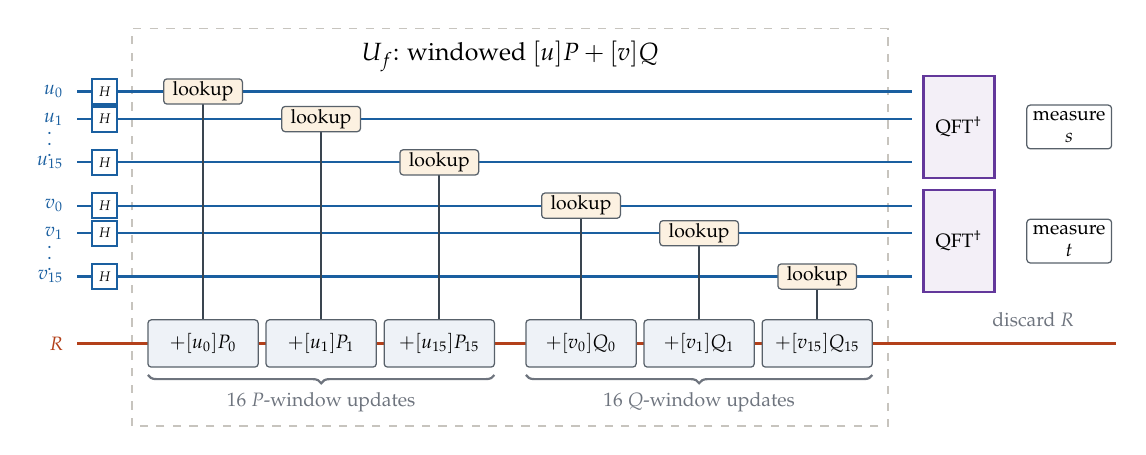
\begin{tikzpicture}[x=1mm,y=1mm]
    \draw[rulegrey,dashed,line width=0.6pt] (15,-10.5) rectangle (111,40);
    \node[font=\small,anchor=north] at (63,39.6) {$U_f$: windowed $[u]P+[v]Q$};
    \foreach \y/\l in {32/u_0,28.5/u_1,23/u_{15},17.5/v_0,14/v_1,8.5/v_{15}} {
      \draw[cwire] (8,\y) -- (114,\y); \node[lab,color=cblue,font=\scriptsize] at (7.5,\y) {$\l$};
      \node[hop,minimum size=3.2mm,font=\tiny] at (11.5,\y) {$H$};}
    \node[color=cblue,font=\scriptsize] at (4.5,26.3) {$\vdots$}; \node[color=cblue,font=\scriptsize] at (4.5,11.8) {$\vdots$};
    \draw[twire] (8,0) -- (140,0); \node[lab,color=cverm,font=\scriptsize] at (7.5,0) {$R$};
    \foreach \x/\y/\a in {24/32/{$+[u_0]P_0$},39/28.5/{$+[u_1]P_1$},54/23/{$+[u_{15}]P_{15}$},72/17.5/{$+[v_0]Q_0$},87/14/{$+[v_1]Q_1$},102/8.5/{$+[v_{15}]Q_{15}$}} {
      \draw[thick,color=body] (\x,\y) -- (\x,3);
      \node[bxl,minimum width=10mm,minimum height=3.2mm,inner sep=0.7pt] at (\x,\y) {lookup};
      \node[bxa,minimum width=14mm,minimum height=6mm,inner sep=0.7pt] at (\x,0) {\a};}
    \draw[decorate,decoration={brace,amplitude=3pt,mirror},thick,color=subtle] (17,-4) -- (61,-4) node[midway,below=2.5pt,font=\scriptsize] {16 $P$-window updates};
    \draw[decorate,decoration={brace,amplitude=3pt,mirror},thick,color=subtle] (65,-4) -- (109,-4) node[midway,below=2.5pt,font=\scriptsize] {16 $Q$-window updates};
    \node[qop,minimum width=9mm,minimum height=13mm,font=\scriptsize] at (120,27.5) {QFT$^\dagger$};
    \node[qop,minimum width=9mm,minimum height=13mm,font=\scriptsize] at (120,13) {QFT$^\dagger$};
    \node[bx,fill=white] at (134,27.5) {measure\\$s$}; \node[bx,fill=white] at (134,13) {measure\\$t$};
    \node[note,anchor=west] at (123,3) {discard $R$};
  \end{tikzpicture}\par
  \vskip1mm
  \raggedright{\small Each window register is the address of one table and leaves $U_f$ unchanged. This is the fully coherent picture; the semiclassical version interleaves the inverse QFT with the windows and recycles the control qubits.}
\end{frame}

\setcounter{framenumber}{95}
\begin{frame}{L5: windows, zig-zag, and one control qubit}
  \begin{columns}[T]
    \begin{column}{0.5\textwidth}
      \small
      \textbf{Windowing}: $w$ control bits address a table of $2^w$ points: $2n+2$ additions become $2\lceil(n+1)/w\rceil$. A lookup ($2^w$ Toffolis) is far cheaper than an addition, so $w=16$.\par\vskip1mm
      \textbf{Zig-zag} (Grassl et al.): runs of $\rho,\rho-1,\dots,1$ additions on $\rho$ registers, undoing all but the last of each run --- $\rho(\rho+1)/2$ additions on $\rho$ registers of projective garbage.\par\vskip1mm
      \textbf{Semiclassical QFT}: both scalar registers become one recycled qubit.
    \end{column}
    \begin{column}{0.46\textwidth}
      \centering
      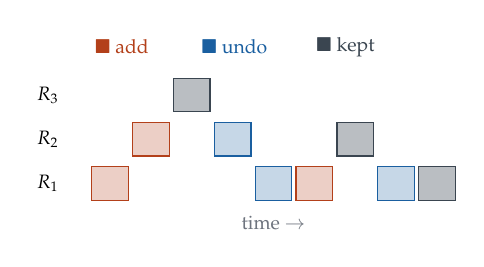
\begin{tikzpicture}[x=5.2mm,y=5.6mm]
        \foreach \r in {1,2,3} \node[lab,font=\scriptsize] at (0,\r) {$R_\r$};
        \foreach \t/\r/\c in {1/1/cverm,2/2/cverm,3/3/cverm,4/2/cblue,5/1/cblue,6/1/cverm,7/2/cverm,8/1/cblue,9/1/cverm} {
          \draw[draw=\c,fill=\c!25] (\t-0.45,\r-0.38) rectangle (\t+0.45,\r+0.38);}
        \draw[draw=body,fill=body!35] (3-0.45,3-0.38) rectangle (3+0.45,3+0.38);
        \draw[draw=body,fill=body!35] (7-0.45,2-0.38) rectangle (7+0.45,2+0.38);
        \draw[draw=body,fill=body!35] (9-0.45,1-0.38) rectangle (9+0.45,1+0.38);
        \node[font=\scriptsize,color=subtle] at (5,0.1) {time $\rightarrow$};
        \node[font=\scriptsize,color=cverm,anchor=west] at (0.4,4.1) {$\blacksquare$ add};
        \node[font=\scriptsize,color=cblue,anchor=west] at (3.0,4.1) {$\blacksquare$ undo};
        \node[font=\scriptsize,color=body,anchor=west] at (5.8,4.1) {$\blacksquare$ kept};
      \end{tikzpicture}\par
      {\scriptsize $\rho=3$: six additions on three registers}
      \vskip1mm
      \footnotesize
      \renewcommand{\arraystretch}{1.08}
      \begin{tabular}{@{}lrrr@{}}
        \toprule
        $n=256$ & none & $w=11$ & $w=16$ \\
        \midrule
        point additions & 514 & 48 & \textbf{34} \\
        zig-zag registers & 32 & 10 & 8 \\
        garbage qubits & 24\,576 & & \textbf{6\,144} \\
        \bottomrule
      \end{tabular}
    \end{column}
  \end{columns}
\end{frame}

\setcounter{framenumber}{96}
\begin{frame}{L5: one windowed addition is seven in-place updates}
  {\small Accumulator $R=(x_R,y_R)$ in registers $X,Y$; looked-up addend $A=(x_A,y_A)$; the result $R'=R+A$ lands in the same $X,Y$.}
  \vskip1mm
  \centering\small
  \renewcommand{\arraystretch}{1.12}
  \begin{tabular}{@{}rlll@{}}
    \toprule
    & update & after it & \texttt{windowed\_padd} \\
    \midrule
    1 & $X\leftarrow x_R-x_A$, \ $Y\leftarrow y_R-y_A$ & $X=d_x$, \ $Y=d_y$ & \# 3, 4 \\
    2 & $Y\leftarrow Y\,X^{-1}$ & $Y=\lambda$ & \# 6, division \\
    3 & $X\leftarrow X+3x_A$ & $X=x_R+2x_A$ & \# 7--9 \\
    4 & $X\leftarrow X-Y^2$ & $X=x_A-x_{R'}$ & \# 10, square \\
    5 & $Y\leftarrow Y\,X$ & $Y=\lambda(x_A-x_{R'})$ & \# 11, multiplication \\
    6 & $Y\leftarrow Y-y_A$ & $Y=y_{R'}$ & \# 14 \\
    7 & $X\leftarrow x_A-X$ & $X=x_{R'}$ & \# 12, 15 \\
    \bottomrule
  \end{tabular}\par
  \vskip2mm
  \raggedright
  \begin{greyblock}[fontupper=\small]
    \textbf{Algebraic check.} \ $\lambda=\dfrac{y_R-y_A}{x_R-x_A}$, \ $x_{R'}=\lambda^2-x_R-x_A$, \ $y_{R'}=\lambda(x_A-x_{R'})-y_A$. After steps 3--4, $X=(x_R-x_A)+3x_A-\lambda^2=x_A-x_{R'}$; steps 5--7 then give $y_{R'}$ and $x_{R'}$ with no separate output registers.
  \end{greyblock}
\end{frame}

\setcounter{framenumber}{97}
\begin{frame}{L5: the same addition as six stages on two registers}
  \centering
  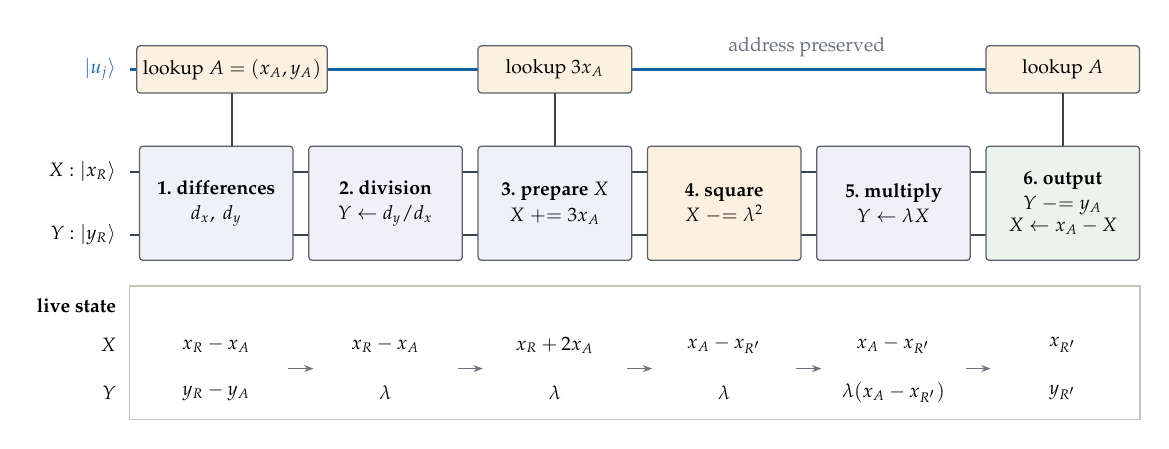
\begin{tikzpicture}[x=1mm,y=1mm]
    \draw[cwire] (14,31) -- (142,31); \node[lab,color=cblue,font=\scriptsize] at (13.5,31) {$|u_j\rangle$};
    \foreach \x/\t in {27/{lookup $A=(x_A,y_A)$},68/{lookup $3x_A$},132.5/{lookup $A$}} {
      \node[bxl,minimum width=19.5mm,minimum height=6mm] at (\x,31) {\t};
      \draw[thick,color=body] (\x,28) -- (\x,21.3);}
    \node[note,anchor=south] at (100,31.4) {address preserved};
    \draw[wire] (14,18) -- (142,18); \node[lab,font=\scriptsize] at (13.5,18) {$X:|x_R\rangle$};
    \draw[wire] (14,10) -- (142,10); \node[lab,font=\scriptsize] at (13.5,10) {$Y:|y_R\rangle$};
    \foreach \i/\x/\c/\t/\f in {1/25/bxa/{differences}/{$d_x,\ d_y$},2/46.5/bxo/{division}/{$Y\leftarrow d_y/d_x$},3/68/bxa/{prepare $X$}/{$X\mathrel{+}=3x_A$},4/89.5/bxl/{square}/{$X\mathrel{-}=\lambda^2$},5/111/bxo/{multiply}/{$Y\leftarrow \lambda X$},6/132.5/bxk/{output}/{$Y\mathrel{-}=y_A$\\$X\leftarrow x_A-X$}} {
      \node[style=\c,minimum width=19.5mm,minimum height=14.5mm] at (\x,14) {\textbf{\i.\ \t}\\[0.4mm]\f};}
    \draw[rulegrey,line width=0.5pt] (14,-13.5) rectangle (142.3,3.5);
    \node[font=\scriptsize\bfseries,anchor=east] at (13.5,1) {live state};
    \node[font=\scriptsize,anchor=east] at (13.5,-4) {$X$}; \node[font=\scriptsize,anchor=east] at (13.5,-10) {$Y$};
    \foreach \x/\a/\b in {25/{x_R-x_A}/{y_R-y_A},46.5/{x_R-x_A}/{\lambda},68/{x_R+2x_A}/{\lambda},89.5/{x_A-x_{R'}}/{\lambda},111/{x_A-x_{R'}}/{\lambda(x_A-x_{R'})},132.5/{x_{R'}}/{y_{R'}}} {
      \node[font=\scriptsize] at (\x,-4) {$\a$}; \node[font=\scriptsize] at (\x,-10) {$\b$};}
    \foreach \x in {35.75,57.25,78.75,100.25,121.75} \draw[-{Stealth[length=1.2mm]},color=subtle] (\x-1.6,-7) -- (\x+1.6,-7);
  \end{tikzpicture}\par
  \vskip1mm
  \raggedright{\small Stages 2 and 5 share one machine, a dialog GCD walk: it produces $\lambda$, then replays a fresh dialog to multiply by $X$. The three lookups are what Act XII makes cheap.}
\end{frame}

\setcounter{framenumber}{98}
\begin{frame}[fragile]{The windowed point addition, in code}
  \code[basicstyle=\ttfamily\fontsize{7.6}{8.8}\selectfont]{windowed_padd.py}
  \begin{columns}[T]
    \begin{column}{0.48\textwidth}
      {\small Step 6 runs the multiplier backwards, step 11 forwards: $\lambda$ is consumed, not cleared by a second division.}
    \end{column}
    \begin{column}{0.48\textwidth}
      {\small $i=0$ is free: $O$ is $(0,0)$ and steps 6 and 11 cancel. Fails only on $x_R=x_P$, $x_3=x_P$, or $x_R=0$ adding $O$.}
    \end{column}
  \end{columns}
\end{frame}

\setcounter{framenumber}{99}
\begin{frame}{Act VIII's optimisations in plain words (1/2)}
  \centering\footnotesize
  \renewcommand{\arraystretch}{1.15}
  \begin{tabular}{@{}>{\raggedright}p{30mm}>{\raggedright}p{63mm}>{\raggedright\arraybackslash\leavevmode\color{cverm}}p{40mm}@{}}
    \toprule
    optimisation & what it does & \color{ink}what it bought \\
    \midrule
    \textbf{L0 temporary AND} & the 4-T trick inside a modular inversion & $2.50\times$ fewer T at every size \\
    \textbf{L1 Gidney adder, copy-then-add} & $n-1$ ANDs instead of $2n$ Toffolis; AND the addend into a clean register under the control, add uncontrolled & controlled add $128\to63$ Toffolis ($n=32$) \\
    \textbf{L2 top-bit, pseudo-Mersenne} & decide ``$\ge p$?'' from a few top bits; for $p=2^{u}-f$, subtracting $p$ is clearing a bit and adding $f$ & doubling $25\to4$ Toffolis; 40--50 top bits at size \\
    \textbf{L3 carry-save Montgomery} & the reduction rewritten to look like a multiplication step: one 3:2 compressor tree does both & depth $\div2.0$ ($n=16$), $4\times$ the qubits \\
    \bottomrule
  \end{tabular}
\end{frame}

\setcounter{framenumber}{100}
\begin{frame}{Act VIII's optimisations in plain words (2/2)}
  \centering\footnotesize
  \renewcommand{\arraystretch}{1.15}
  \begin{tabular}{@{}>{\raggedright}p{30mm}>{\raggedright}p{63mm}>{\raggedright\arraybackslash\leavevmode\color{cverm}}p{40mm}@{}}
    \toprule
    optimisation & what it does & \color{ink}what it bought \\
    \midrule
    \textbf{L3 Kaliski, late reduction} & run every round, reduce once at the end: doublings become wire renamings & $-29\%$ Toffolis, $-41\%$ depth ($n=12$) \\
    \textbf{L3 Euclidean dialog, replay} & keep two decision bits per GCD round, replay them linearly on any pair: inversion and multiplication in one & $-54\%$ Toffolis, $-43\%$ qubits ($p=61$) \\
    \textbf{L4 Jacobian coordinates} & projective coordinates trade the division for 11 multiplications & $-45\%$ Toffolis; $3n$ qubits of garbage \\
    \textbf{L5 windows, zig-zag, one control} & 16-bit windows, a schedule that bounds live garbage, and the semiclassical QFT & $514\to34$ additions; garbage $24\,576\to6\,144$ \\
    \bottomrule
  \end{tabular}
  \par\vskip1mm{\scriptsize\color{subtle}Each measured on a fixed task at a toy size, correctness re-checked in the benchmark.}
\end{frame}

\setcounter{framenumber}{101}
\begin{frame}{Everything at once: how the savings compose}
  \begin{columns}[T]
    \begin{column}{0.5\textwidth}
      \centering\footnotesize
      \renewcommand{\arraystretch}{1.1}
      \begin{tabular}{@{}lrrr@{}}
        \toprule
        $p=7$ & Toffoli & qubits & \\
        \midrule
        affine, in place & 2\,756 & 64 & \\
        Jacobian & 1\,544 & 75 & $-44\%$ \\
        windowed, dialog & 1\,523 & 49 & $-45\%$ \\
        \bottomrule
      \end{tabular}\par
      {\scriptsize one point addition}\par
      \vskip2mm
      \raggedright\small
      Whole circuit, $y^2=x^3+5x+4 \bmod 7$: \textbf{69 qubits, 105\,339 gates} with real arithmetic; with a permutation oracle 12 qubits, or 7 with one recycled control qubit.
    \end{column}
    \begin{column}{0.46\textwidth}
      \small
      \begin{itemize}\setlength{\itemsep}{1mm}
        \item \textbf{Gate level, partly one saving}: Gidney adder and temporary AND are one idea counted twice; pseudo-Mersenne ($6.2\times$) composes.
        \item \textbf{Structural, pick one}: the dialog and Jacobian coordinates both answer the inversion.
        \item \textbf{Count level, multiply}: windows $\div15$ additions, zig-zag $\div4$ garbage, the semiclassical QFT deletes both counting registers.
      \end{itemize}
    \end{column}
  \end{columns}
  \begin{takeaway}Halving a point addition is worth half as much as running fifteen times fewer of them.\end{takeaway}
\end{frame}

\setcounter{framenumber}{102}
\begin{frame}{ECDLP optimisations, measured}
  \begin{columns}[c]
    \begin{column}{0.62\textwidth}
      \centering\fig[width=\textwidth]{ablation.pdf}
    \end{column}
    \begin{column}{0.34\textwidth}
      \small
      From eprints 2026/106 and 2026/1128, each on a fixed task, correctness re-checked.
      \vskip2mm
      Pseudo-Mersenne doubling is approximate (3\% failures); Jacobian coordinates leave $3n$ garbage qubits per addition; the carry-save multiplier trades $4\times$ the qubits for depth.
    \end{column}
  \end{columns}
  \resolved{The same circuit solves the ECDLP; the division makes its box costlier --- and all Toffolis.}
\end{frame}

% ======================================================================
\act{Optimisations in detail --- secp256k1 at full size (Act XII)}

\setcounter{framenumber}{164}
\begin{frame}{How every optimisation is checked}
  \begin{columns}[T]
    \begin{column}{0.42\textwidth}
      \blocktitle{A switch, not a fork}
      Each optimisation is a switch beside the construction it refines. Switch it off and the circuit is the old one, gate for gate.
      \vskip3mm
      \blocktitle{Exhaustively, at toy primes}
      Every basis input, every ancilla back to $|0\rangle$; a regression test pins every gate count quoted here.
    \end{column}
    \begin{column}{0.54\textwidth}
      \begin{greyblock}
        \blocktitle{Measurements leave phases}
        The exhaustive simulator cannot see phases, so each gate carries a unitary definition for the tests and a measurement-based \emph{price}. A sparse state-vector simulator runs the real measure-and-repair and checks that every basis input returns with the same phase. An approximate repair fails exactly on the inputs the tests predict.
      \end{greyblock}
    \end{column}
  \end{columns}
\end{frame}

\setcounter{framenumber}{165}
\begin{frame}{1. Lookups: ten recomputed $\to$ three loads and one repair}
  \centering
  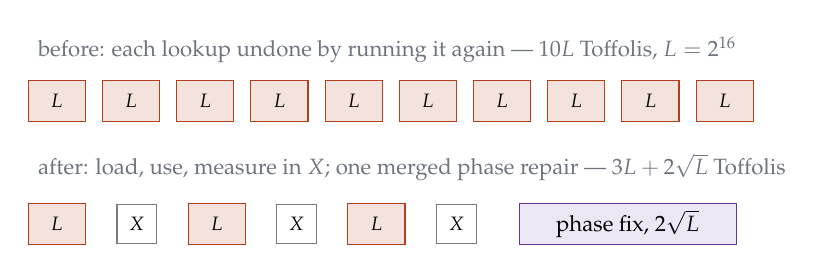
\begin{tikzpicture}[x=1.45mm,y=1.3mm,font=\footnotesize]
    \node[anchor=west,color=subtle] at (0,15) {before: each lookup undone by running it again --- $10L$ Toffolis, $L=2^{16}$};
    \foreach \i in {0,...,9}{\draw[fill=cverm!15,draw=cverm] (\i*6.5,8) rectangle (\i*6.5+5,12);
      \node[font=\scriptsize] at (\i*6.5+2.5,10) {$L$};}
    \node[anchor=west,color=subtle] at (0,3.5) {after: load, use, measure in $X$; one merged phase repair --- $3L+2\sqrt L$ Toffolis};
    \foreach \i in {0,1,2}{\draw[fill=cverm!15,draw=cverm] (\i*14,-4) rectangle (5+\i*14,0);
      \node[font=\scriptsize] at (2.5+\i*14,-2) {$L$};
      \node[meter,minimum size=5mm,font=\scriptsize] at (9.5+\i*14,-2) {$X$};}
    \draw[fill=cpurple!12,draw=cpurple] (43,-4) rectangle (62,0); \node at (52.5,-2) {phase fix, $2\sqrt L$};
  \end{tikzpicture}
  \vskip3mm
  \begin{columns}[T]
    \begin{column}{0.58\textwidth}
      \raggedright $X$-measuring a loaded register costs nothing but leaves the phase $(-1)^{m\cdot T[a]}$ on the address. A \emph{phase lookup} of $F[a]=m\cdot T[a]$ repairs it in $\approx2\sqrt L$ ANDs, against $L$ for a lookup. IonQ's step: the three unloads share one address, so their tables are XORed and one repair serves all three.
    \end{column}
    \begin{column}{0.38\textwidth}
      \begin{peachblock}\peachtitle{Measured, $n=256$, $w=16$}
        $1\,310\,700\to\mathbf{197\,364}$ Toffolis per addition.
      \end{peachblock}
    \end{column}
  \end{columns}
\end{frame}

\setcounter{framenumber}{166}
\begin{frame}[fragile]{2. The GCD: conditionally inverted steps}
  \begin{columns}[T]
    \begin{column}{0.53\textwidth}
      Two thirds of a point addition is the in-place multiplier, most of it the walk and replay of a binary GCD.
      \vskip2mm
      IonQ store $\tilde v=v+(1-a)u$, $a=v\bmod2$: both registers stay odd, the next parity is two CNOTs, and each update $\tilde v\leftarrow(\tilde v\pm u)/2$ is one \emph{uncontrolled} adder between two rows of CNOTs.
    \end{column}
    \begin{column}{0.43\textwidth}
      \code[basicstyle=\ttfamily\footnotesize]{ci_add.py}
      \vskip1mm
      {\small $n-1$ ANDs, where [1128] spends $2n$ on a controlled subtraction. The recorded bits are exactly the dialog's, so its replay and packing carry over.}
      \begin{peachblock}\peachtitle{Measured, $n=256$}
        in-place multiplication: $1\,955\,276\to\mathbf{720\,565}$
      \end{peachblock}
    \end{column}
  \end{columns}
\end{frame}

\setcounter{framenumber}{167}
\begin{frame}{Five GCDs behind one interface}
  \centering\small
  \renewcommand{\arraystretch}{1.15}
  \begin{tabular}{@{}lrr@{}}
    \toprule
    in-place multiplication, $n=256$ & rounds & Toffolis \\
    \midrule
    dialog [1128], exact, full width & 401 & 1\,955\,276 \\
    $+$ fused 77-bit compares, width schedule, pseudo-Mersenne & 401 & 865\,588 \\
    conditionally inverted (IonQ), IonQ replay & 401 & \textbf{720\,565} \\
    ping-pong (ECDSA.Fail) & 704 & 917\,565 \\
    Jump-2 (ECDSA.Fail) & 261 & 1\,161\,099 \\
    \bottomrule
  \end{tabular}
  \vskip3mm
  \raggedright \texttt{ec\_gcd.py} holds [1128]'s dialog, IonQ's conditionally inverted walk, and ECDSA.Fail's ping-pong and Jump-2 (with its base-5 transcript codec).
  \begin{takeaway}Ping-pong is cheapest per round but needs $2.75n$ rounds --- and exhaustively, $n=16$ needs $3.9n$.\end{takeaway}
\end{frame}

\setcounter{framenumber}{168}
\begin{frame}{The GCD, as a circuit: walk, record, replay}
  \centering
  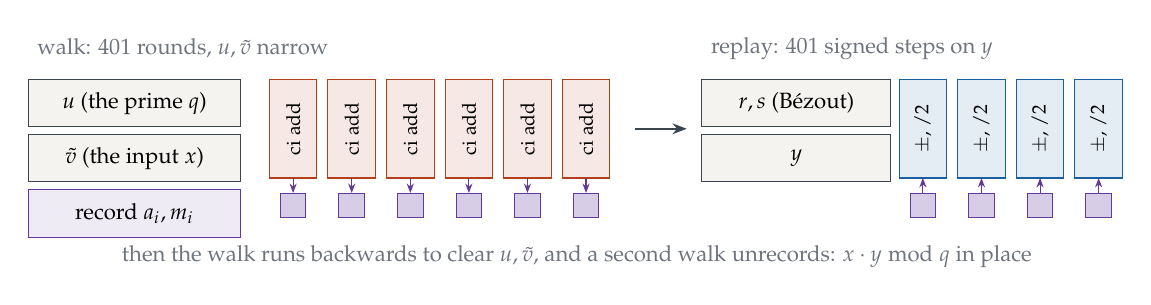
\begin{tikzpicture}[x=0.93mm,y=1.0mm,font=\footnotesize]
    \tikzset{reg/.style={draw=body,fill=greybox,minimum height=6mm,anchor=west,inner sep=2pt}}
    \node[reg,minimum width=27mm] (u) at (0,16) {$u$ (the prime $q$)};
    \node[reg,minimum width=27mm] (v) at (0,9) {$\tilde v$ (the input $x$)};
    \node[reg,minimum width=27mm,fill=cpurple!10,draw=cpurple] (r) at (0,2) {record $a_i,m_i$};
    \foreach \i in {0,...,5}{
      \pgfmathsetmacro{\x}{33+\i*8}
      \draw[fill=cverm!12,draw=cverm] (\x,6.5) rectangle (\x+6.5,19); \node[rotate=90,font=\scriptsize] at (\x+3.25,12.75) {ci add};
      \draw[cpurple,-{Stealth[length=1.2mm]}] (\x+3.25,6.5) -- (\x+3.25,4.6);
      \draw[fill=cpurple!25,draw=cpurple] (\x+1.5,1.5) rectangle (\x+5,4.5);}
    \node[color=subtle,anchor=west] at (0,23) {walk: 401 rounds, $u,\tilde v$ narrow};
    \draw[-{Stealth[length=1.8mm]},thick,color=body] (83,12.75) -- (90,12.75);
    \node[reg,minimum width=24mm] (s) at (92,16) {$r,s$ (Bézout)};
    \node[reg,minimum width=24mm] (y) at (92,9) {$y$};
    \foreach \i in {0,...,3}{
      \pgfmathsetmacro{\x}{119+\i*8}
      \draw[fill=cblue!12,draw=cblue] (\x,6.5) rectangle (\x+6.5,19); \node[rotate=90,font=\scriptsize] at (\x+3.25,12.75) {$\pm$, $/2$};
      \draw[cpurple,-{Stealth[length=1.2mm]}] (\x+3.25,4.6) -- (\x+3.25,6.5);
      \draw[fill=cpurple!25,draw=cpurple] (\x+1.5,1.5) rectangle (\x+5,4.5);}
    \node[color=subtle,anchor=west] at (92,23) {replay: 401 signed steps on $y$};
    \node[color=subtle] at (75,-3.5) {then the walk runs backwards to clear $u,\tilde v$, and a second walk unrecords: $x\cdot y\bmod q$ in place};
  \end{tikzpicture}
  \vskip3mm
  \raggedright\small
  \begin{itemize}
    \item The record is packed 5 Toffolis a round ([1128] Fig.~1) and grows into the qubits the narrowing walk frees: \emph{register sharing}.
    \item IonQ's replay cells: a phase-approximate adder whose carry is the reduction flag, 352 Toffolis a step against 712.
    \item It cannot see $x+y=p$, met once in the first 37 steps: those keep an exact ``careful'' cell.
  \end{itemize}
\end{frame}

\setcounter{framenumber}{169}
\begin{frame}{3. Squaring: a dedicated squarer and a pseudo-Mersenne fold}
  \begin{columns}[T]
    \begin{column}{0.52\textwidth}
      Step 10 subtracts $\lambda^2$; with the general multiplier that is two multiplications. IonQ's squarer:
      \[ x^2=-x+\sum_i(2x_i-1)\,2^{2i+1}(h_i+x_i) \]
      with $h_i=\lfloor x/2^{i+1}\rfloor$. Every term is an \emph{unconditional} signed subtraction on a window of $n+1-i$ bits: $\tfrac12n(n+3)$ ANDs. A fold $2^{256}\equiv2^{32}+977$ reduces into the accumulator.
    \end{column}
    \begin{column}{0.44\textwidth}
      \centering
      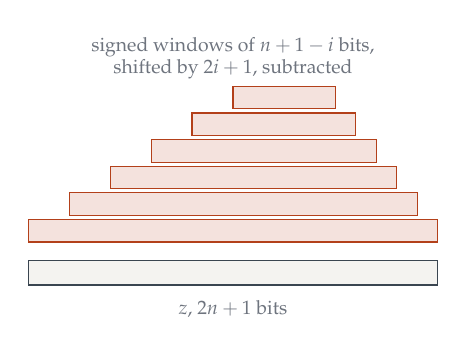
\begin{tikzpicture}[x=1.3mm,y=1.3mm,font=\scriptsize]
        \draw[fill=greybox,draw=body] (0,-1.2) rectangle (40,1.2); \node[color=subtle] at (20,-3.5) {$z$, $2n+1$ bits};
        \foreach \i in {0,...,5}{\draw[fill=cverm!15,draw=cverm] (\i*4,3+\i*2.6) rectangle (40-\i*2,5.2+\i*2.6);}
        \node[color=subtle,align=center] at (20,21) {signed windows of $n+1-i$ bits,\\shifted by $2i+1$, subtracted};
      \end{tikzpicture}
      \begin{peachblock}\peachtitle{Measured, $n=256$}
        square-subtract: $1\,050\,623\to\mathbf{79\,160}$ Toffolis.
      \end{peachblock}
    \end{column}
  \end{columns}
\end{frame}

\setcounter{framenumber}{170}
\begin{frame}[fragile]{The squarer, in code}
  \code[basicstyle=\ttfamily\footnotesize]{sqr_int.py}
  \vskip2mm
  Row $i$: flip $h$ by $x_i$ so the operand is $\pm(h_i+x_i)$ with sign $x_i$, subtract it from the window of $z$ at offset $2i+1$, flip back.
\end{frame}

\setcounter{framenumber}{171}
\begin{frame}[fragile]{Building 256 bits on a laptop: one gate per shape}
  \small One 256-bit point addition is tens of millions of gates but few distinct pieces: the replay calls one modular adder 800 times. \texttt{hier.tracing()} wraps the existing builders; each call is built once per \emph{shape} and appended as one opaque gate.\par
  \vskip1mm
  \code[basicstyle=\ttfamily\fontsize{7.6}{8.8}\selectfont]{boundary.py}
  \begin{columns}[T]
    \begin{column}{0.48\textwidth}
      {\small \textbf{Shape}: register widths, shared qubits, classical parameters. Run backwards, the gate is inverted.}
    \end{column}
    \begin{column}{0.48\textwidth}
      {\small \textbf{Checked}: equal to the flat count at toy size (8 configurations); Qualtran agrees on the exported bloqs.}
    \end{column}
  \end{columns}
\end{frame}

\setcounter{framenumber}{172}
\begin{frame}{The first full-size builds}
  \centering\footnotesize
  \renewcommand{\arraystretch}{1.12}
  \begin{tabular}{@{}lrr@{}}
    \toprule
    one windowed point addition, secp256k1, $w=16$ & Toffolis & qubits \\
    \midrule
    Qualtran's \texttt{ECAdd} (Litinski 2023), for reference & 8\,346\,972 & 1\,798 \\
    dialog [1128], exact arithmetic, MBU lookups & 5\,163\,617 & 2\,104 \\
    \quad $+$ 77-bit comparisons, width schedule, pseudo-Mersenne replay & 2\,972\,327 & 2\,251 \\
    \quad $+$ dedicated squarer and fold & 2\,000\,864 & 2\,251 \\
    conditionally inverted walk and replay (IonQ), squarer & \textbf{1\,711\,194} & 2\,251 \\
    ping-pong walk, 704 rounds (ECDSA.Fail), squarer & 2\,117\,534 & 2\,155 \\
    dialog, register sharing, Fig.~1 packing, squarer & 2\,006\,184 & \textbf{1\,873} \\
    \bottomrule
  \end{tabular}\par
  \vskip2mm
  \raggedright\small
  The whole algorithm builds too: 28 windowed additions, $47\,978\,966$ Toffolis on $2\,251$ qubits. On the same tree Qualtran counts $249\,846\,912$ Cliffords and $29\,873\,480$ measurements.
  \begin{takeaway}Two gaps remain: the best row is $23\%$ above IonQ's count, and every row needs more qubits than any paper reports.\end{takeaway}
\end{frame}

\setcounter{framenumber}{173}
\begin{frame}{4. Matching IonQ: the gap is in the replay}
  \begin{columns}[T]
    \begin{column}{0.55\textwidth}
      \centering\footnotesize
      \renewcommand{\arraystretch}{1.12}
      \begin{tabular}{@{}lrr@{}}
        \toprule
        $n=256$, Toffolis & before & after \\
        \midrule
        lookups, repair & 197\,364 & 197\,364 \\
        GCD walks, undone & 593\,432 & 593\,432 \\
        Bézout replays & 833\,312 & \textbf{564\,086} \\
        \quad of which signed additions & 569\,600 & 307\,574 \\
        square-subtract & 79\,160 & 79\,160 \\
        everything else & 7\,926 & 4\,571 \\
        \midrule
        one point addition & 1\,711\,194 & \textbf{1\,438\,613} \\
        \bottomrule
      \end{tabular}
    \end{column}
    \begin{column}{0.41\textwidth}
      \small The walk is already IonQ's; the replay is not. Each of its 800 steps adds $\pm r$ into $s$ modulo $p$, and the cell that did it costs \textbf{712} Toffolis --- of which only 256 are the addition.
      \vskip2mm
      The rest are top-bit tests: does the sum need reducing, is it exactly $p$, was the input $0$?
    \end{column}
  \end{columns}
  \vskip2mm
  {\small\raggedright After: $1\,426\,965$ executed, within $2.5\%$ of IonQ's $1\,392\,608$. The 28-addition algorithm: $40\,346\,698$ Toffolis, against IonQ's $39.0\times10^6$.\par}
\end{frame}

\setcounter{framenumber}{174}
\begin{frame}{IonQ's modular adder: the carry \emph{is} the flag}
  \centering
  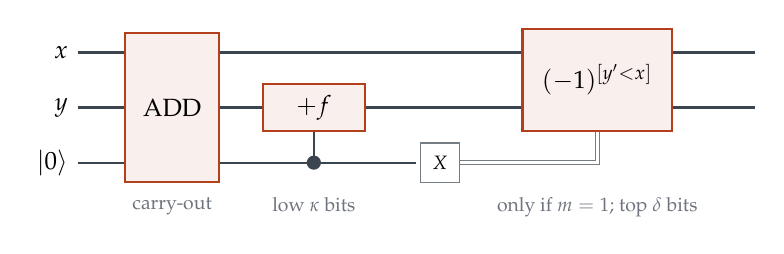
\begin{tikzpicture}[x=10mm,y=7mm]
    \foreach \y/\l in {2/{$x$},1/{$y$},0/{$|0\rangle$}} {\node[lab] at (0,\y) {\l};}
    \draw[wire] (0,2) -- (8.6,2); \draw[wire] (0,1) -- (8.6,1); \draw[wire] (0,0) -- (4.3,0);
    \node[op,minimum width=12mm,minimum height=19mm] at (1.2,1) {ADD};
    \node[note,anchor=north] at (1.2,-0.45) {carry-out};
    \draw[thick,color=body] (3,0) -- (3,0.7); \node[dot] at (3,0) {};
    \node[op,minimum width=13mm,minimum height=6mm] at (3,1) {$+f$};
    \node[note,anchor=north] at (3,-0.45) {low $\kappa$ bits};
    \node[meter] (m) at (4.6,0) {$X$};
    \draw[clw] (m.east) -- (6.6,0) -- (6.6,0.85);
    \node[op,minimum width=19mm,minimum height=13mm] at (6.6,1.5) {$(-1)^{[y'<x]}$};
    \node[note,anchor=north] at (6.6,-0.45) {only if $m=1$; top $\delta$ bits};
  \end{tikzpicture}
  \vskip3mm
  \raggedright
  \begin{columns}[T]
    \begin{column}{0.48\textwidth}
      \small If $x+y\ge2^{256}$ the carry is set, and subtracting $p$ is ``drop the carry, add $f=2^{32}+977$'': only the low $\kappa=65$ bits move. No test decides the reduction.
    \end{column}
    \begin{column}{0.48\textwidth}
      \small After the correction the carry equals $[y'<x]$: reduced, $y'=x+y-p<x$; not, $y'\ge x$. So it is $X$-measured, and half the time a $\delta=32$-bit comparator repairs the phase.
    \end{column}
  \end{columns}
  \begin{takeaway}352 Toffolis worst case, 336 counting what executes (IonQ's convention), against 712.\end{takeaway}
\end{frame}

\setcounter{framenumber}{175}
\begin{frame}[fragile]{IonQ's modular adder, in code}
  \code[basicstyle=\ttfamily\fontsize{7.6}{8.8}\selectfont]{modadd_pm_phase.py}
  \begin{columns}[T]
    \begin{column}{0.48\textwidth}
      {\small Approximate only to order $f/p$ or $2^{-\delta}$: sums in $[p,2^{256})$, a carry past bit $\kappa$, a tie in the top $\delta$ bits.}
    \end{column}
    \begin{column}{0.48\textwidth}
      {\small At toy primes: wrong on exactly the sums in $[p,2^n)$, phase-correct everywhere else, every measurement performed.}
    \end{column}
  \end{columns}
\end{frame}

\setcounter{framenumber}{176}
\begin{frame}{The one case that is not rare: 37 careful steps}
  \begin{columns}[c]
    \begin{column}{0.5\textwidth}
      \small The replay must pass through $0$. Dividing, the first swap moves a $0$ into $s$, and complementing it gives $2^{256}-1$, not a residue. Multiplying, the same step adds $x+y=p$ exactly: the one sum the carry cannot see.
      \vskip2mm
      The step is fixed by the 2-adic valuation of $x$: within the first $k$ steps with probability $1-2^{-k}$. So the first 37 steps keep the exact cell (IonQ: ``rounds with $x+y=p$: 37'').
    \end{column}
    \begin{column}{0.46\textwidth}
      \centering
      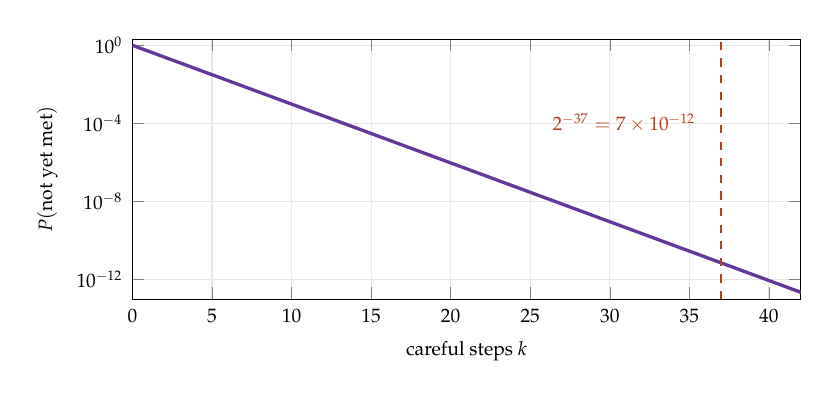
\begin{tikzpicture}
        \begin{axis}[scale only axis,width=0.7\linewidth,height=3.3cm,ymode=log,xmin=0,xmax=42,ymin=1e-13,ymax=2,
          xlabel={careful steps $k$},ylabel={$P(\text{not yet met})$},ytick={1,1e-4,1e-8,1e-12},
          grid=major,tick label style={font=\scriptsize},label style={font=\scriptsize}]
          \addplot[very thick,cpurple,domain=0:42,samples=43] {2^(-x)};
          \draw[cverm,thick,dashed] (axis cs:37,1e-13) -- (axis cs:37,2);
          \node[font=\scriptsize,cverm,anchor=east] at (axis cs:36,1e-4) {$2^{-37}=7\times10^{-12}$};
        \end{axis}
      \end{tikzpicture}\par
      {\scriptsize measured: the failure rate halves per careful step, zero at 37}
    \end{column}
  \end{columns}
  \vskip2mm
  {\small Multiplying gets its \textbf{own} replay: the inverse of ``measure, sometimes repair'' is ``recompute'', which always runs. Signed additions $569\,600\to307\,574$.}
\end{frame}

\setcounter{framenumber}{177}
\begin{frame}{Signed windows: half the table, and never $O$}
  \begin{columns}[c]
    \begin{column}{0.5\textwidth}
      \centering
      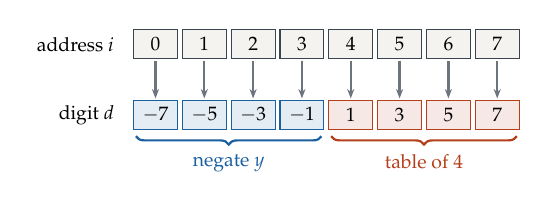
\begin{tikzpicture}[x=6.2mm,y=6mm]
        \node[lab,font=\scriptsize] at (-0.2,1.5) {address $i$};
        \node[lab,font=\scriptsize] at (-0.2,0) {digit $d$};
        \foreach \i/\dd in {0/-7,1/-5,2/-3,3/-1,4/1,5/3,6/5,7/7} {
          \draw[draw=body,fill=greybox] (\i,1.2) rectangle (\i+0.9,1.8); \node[font=\scriptsize] at (\i+0.45,1.5) {\i};
          \draw[thick,-{Stealth[length=1.2mm]},color=subtle] (\i+0.45,1.15) -- (\i+0.45,0.35);
          \ifnum\i<4 \draw[draw=cblue,fill=cblue!12] (\i,-0.3) rectangle (\i+0.9,0.3); \else \draw[draw=cverm,fill=cverm!12] (\i,-0.3) rectangle (\i+0.9,0.3); \fi
          \node[font=\scriptsize] at (\i+0.45,0) {$\dd$};}
        \draw[decorate,decoration={brace,amplitude=3pt,mirror},thick,color=cblue] (0.05,-0.45) -- (3.85,-0.45) node[midway,below=3pt,font=\scriptsize,color=cblue] {negate $y$};
        \draw[decorate,decoration={brace,amplitude=3pt,mirror},thick,color=cverm] (4.05,-0.45) -- (7.85,-0.45) node[midway,below=3pt,font=\scriptsize,color=cverm] {table of 4};
      \end{tikzpicture}\par
      \vskip1mm
      {\scriptsize $w=3$: $d=2i+1-2^w$, looked up by $|d|$ on $w-1$ bits}
    \end{column}
    \begin{column}{0.46\textwidth}
      \small Read the $w$ address bits as an odd digit. The lookup runs over $|d|$; the sign is a negation of $y$ before and after, and consecutive windows merge theirs into one, controlled by the XOR of the signs.
      \vskip2mm
      $2^{15}$ entries instead of $2^{16}$, and odd digits never give $O$.
    \end{column}
  \end{columns}
  \vskip3mm
  \begin{peachblock}[fontupper=\small]\peachtitle{Measured, $n=256$}
    One addition: $1\,340\,563$ Toffolis, $1\,328\,915$ executed --- $4.6\%$ below IonQ; $2\,745\,400$ fewer over the 28 additions.
  \end{peachblock}
\end{frame}

\setcounter{framenumber}{178}
\begin{frame}[fragile]{Signed windows, in code --- and the condition they need}
  \code[basicstyle=\ttfamily\fontsize{7.6}{8.8}\selectfont]{signed.py}
  \begin{columns}[T]
    \begin{column}{0.48\textwidth}
      {\small Needs $y\neq0$: every visited point of odd order. secp256k1 has prime order.}
    \end{column}
    \begin{column}{0.48\textwidth}
      {\small Order-43 curve, every input: one run finds $k$ $43\%$ of the time (ideal $77\%$).}
    \end{column}
  \end{columns}
\end{frame}

\setcounter{framenumber}{179}
\begin{frame}{IonQ's count, then IonQ's width, in one table}
  \centering\small
  \renewcommand{\arraystretch}{1.15}
  \begin{tabular}{@{}lrrr@{}}
    \toprule
    one windowed point addition, secp256k1 & Toffolis & executed & qubits \\
    \midrule
    IonQ-style walk and replay, squarer & 1\,711\,194 & 1\,711\,194 & 2\,251 \\
    $+$ phase-approximate adder in the replay & 1\,441\,968 & 1\,430\,352 & 2\,233 \\
    $+$ signed windows ($2^{15}$-entry tables) & 1\,340\,563 & 1\,328\,915 & 2\,233 \\
    $+$ packing, sharing, lean cells, CNOT ends & 1\,338\,469 & 1\,326\,821 & \textbf{1\,457} \\
    $+$ SELECT-SWAP on the $3x$ lookup & \textbf{1\,322\,341} & \textbf{1\,310\,693} & \textbf{1\,457} \\
    \midrule
    published: IonQ & & 1\,392\,608 & 1\,457 \\
    \bottomrule
  \end{tabular}
  \begin{takeaway}Whole ECDLP-256: \textbf{37\,084\,197 Toffolis (36\,758\,053 executed) on 1\,457 qubits}, 5.9\% below IonQ per addition.\end{takeaway}
\end{frame}

\setcounter{framenumber}{180}
\begin{frame}{Where the 1\,457 qubits go}
  \centering
  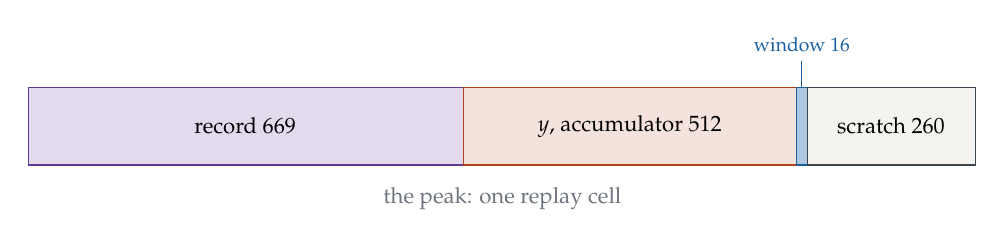
\begin{tikzpicture}[x=1.65mm,y=1.65mm,font=\footnotesize]
    \draw[fill=cpurple!18,draw=cpurple] (0,0) rectangle (33.5,6); \node at (16.7,3) {record 669};
    \draw[fill=cverm!15,draw=cverm] (33.5,0) rectangle (59.1,6); \node at (46.3,3) {$y$, accumulator 512};
    \draw[fill=cblue!35,draw=cblue] (59.1,0) rectangle (60,6);
    \draw[fill=greybox,draw=body] (60,0) rectangle (72.9,6); \node at (66.4,3) {scratch 260};
    \draw[cblue] (59.55,6) -- (59.55,8) node[above,font=\scriptsize] {window 16};
    \node[anchor=north,color=subtle] at (36.5,-1) {the peak: one replay cell};
  \end{tikzpicture}
  \vskip3mm
  \raggedright
  The peak moved four times, and none of the fixes adds a Toffoli:
  \begin{itemize}
    \item the careful cell's scratch is freed after its adder (259 qubits, not 647);
    \item the replay's opening and closing copies are $n$ CNOTs, not exact modular additions;
    \item the fold's 8 subtractions run on the phase adder;
    \item the walk's $u$ is shared with the record.
  \end{itemize}
\end{frame}

\setcounter{framenumber}{181}
\begin{frame}{5. SELECT-SWAP lookups: trade qubits that are free anyway}
  \begin{columns}[T]
    \begin{column}{0.5\textwidth}
      \small A lookup over the high $w-k$ address bits writes $2^k$ words at once; $k$ layers of Fredkins on the low bits move the addressed one into place: $2^{w-k}-2$ ANDs $+(2^k-1)b$ Fredkins.
      \vskip2mm
      The other words are a known function of the address: $X$-measured into the merged repair. The extra qubits live only during the load; at the $3x$ load only 798 are live, so $k=1$ is free under the $1\,457$ peak.
    \end{column}
    \begin{column}{0.46\textwidth}
      \centering
      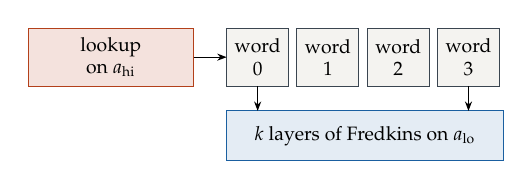
\begin{tikzpicture}[x=1.05mm,y=1.05mm,font=\scriptsize]
        \draw[fill=cverm!15,draw=cverm] (0,10) rectangle (20,17); \node[align=center] at (10,13.5) {lookup\\on $a_{\mathrm{hi}}$};
        \foreach \j in {0,1,2,3}{\draw[fill=greybox,draw=body] (24+\j*8.5,10) rectangle (31.5+\j*8.5,17); \node[align=center] at (27.75+\j*8.5,13.5) {word\\\j};}
        \draw[-{Stealth[length=1.2mm]}] (20,13.5) -- (24,13.5);
        \draw[fill=cblue!12,draw=cblue] (24,1) rectangle (57.5,7); \node at (40.75,4) {$k$ layers of Fredkins on $a_{\mathrm{lo}}$};
        \draw[-{Stealth[length=1.2mm]}] (27.75,10) -- (27.75,7); \draw[-{Stealth[length=1.2mm]}] (53.25,10) -- (53.25,7);
      \end{tikzpicture}
      \vskip2mm
      \footnotesize
      \renewcommand{\arraystretch}{1.1}
      \begin{tabular}{@{}lrrr@{}}
        \toprule
        $k$ (points, $3x$) & qubits & Toffolis & executed \\
        \midrule
        (0, 0) & 1\,457 & 1\,338\,469 & 1\,326\,821 \\
        (0, 1) & \textbf{1\,457} & 1\,322\,341 & \textbf{1\,310\,693} \\
        (1, 1) & 1\,565 & 1\,290\,597 & 1\,278\,949 \\
        (2, 2) & 2\,588 & 1\,268\,581 & 1\,256\,933 \\
        (3, 3) & 4\,635 & 1\,261\,413 & 1\,249\,765 \\
        \bottomrule
      \end{tabular}
    \end{column}
  \end{columns}
\end{frame}

\setcounter{framenumber}{182}
\begin{frame}[fragile]{SELECT-SWAP, in code}
  \code[basicstyle=\ttfamily\footnotesize]{select_swap.py}
  \vskip2mm
  Layer $i$ swaps block $j$ with block $j+2^i$ when address bit $i$ is set: after $k$ layers block 0 holds the addressed word. \texttt{unlookup} measures all blocks out and repairs the phases in one pass.
\end{frame}

\setcounter{framenumber}{183}
\begin{frame}{6. Fewer qubits: $1\,246$ on lean cells, $851$ on three field registers}
  \centering\small
  \renewcommand{\arraystretch}{1.15}
  \begin{tabular}{@{}lrr@{}}
    \toprule
    one windowed point addition; each row adds one option & qubits & Toffolis \\
    \midrule
    IonQ-style (cond.-inverted walk, PM arithmetic) & 2\,251 & 1\,711\,194 \\
    $+$ Fig.~1 packing, replay in $x$'s qubits & 1\,863 & 1\,716\,514 \\
    $+$ CDKM (1-ancilla) adders in replay, squarer, point adds & 1\,389 & 2\,335\,990 \\
    $+$ CDKM dialog walk, lean replay cells, CDKM squarer & 1\,246 & 2\,935\,857 \\
    $+$ Gidney adders where there is headroom, SELECT-SWAP & \textbf{1\,246} & \textbf{2\,821\,091} \\
    $+$ Luo's register-shared EEA instead of the dialog & 1\,107 & 86\,033\,905 \\
    three field registers (Luo et al.\ Sec.~5), signed windows & \textbf{851} & 85\,204\,396 \\
    \bottomrule
  \end{tabular}
  \vskip2mm
  \raggedright{\small $1\,246=4.87n$: record 669, $y$ and accumulator 512, window 16, scratch 38 ([1128]: $4.355n+O(\sqrt n)=1\,192$; IonQ 1\,457; Luo et al.\ 835).}
\end{frame}

\setcounter{framenumber}{184}
\begin{frame}{Chasing the peak: take the scratch out of whatever sets it}
  \begin{columns}[T]
    \begin{column}{0.47\textwidth}
      \centering
      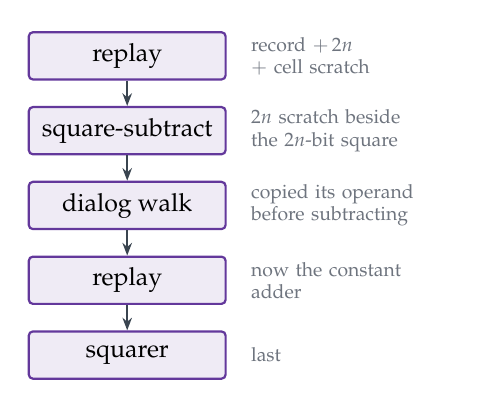
\begin{tikzpicture}[y=9.5mm,
          pk/.style={draw=cpurple,fill=cpurple!10,thick,rounded corners=1.5pt,minimum width=25mm,minimum height=6mm,font=\small},
          why/.style={font=\scriptsize,color=subtle,anchor=west,align=left,text width=26mm}]
        \foreach \y/\t/\w in {4/replay/{record $+\,2n$\\$+$ cell scratch},3/square-subtract/{$2n$ scratch beside\\the $2n$-bit square},2/dialog walk/{copied its operand\\before subtracting},1/replay/{now the constant\\adder},0/squarer/{last}} {
          \node[pk] (n\y) at (0,\y) {\t};
          \node[why] at (1.45,\y) {\w};}
        \foreach \a/\b in {4/3,3/2,2/1,1/0} \draw[-{Stealth[length=1.6mm]},thick,color=body] (n\a) -- (n\b);
      \end{tikzpicture}\par
      {\scriptsize where the peak sat, in the order it moved}\par
      \vskip3mm
      \raggedright{\small Each new cell gives the output of the one it replaces on every input tried, failures included.}
    \end{column}
    \begin{column}{0.49\textwidth}
      \small The qubit count is a statement about \emph{one moment}; every other step can borrow.
      \vskip2mm
      \blocktitle{The cells that come out}
      \begin{itemize}\setlength{\itemsep}{0.6mm}
        \item CDKM adders where no ancilla is free;
        \item a comparator on the CDKM carry chain: 1 ancilla, not $k$;
        \item an all-ones test in $\sqrt k$ chunks, ANDs parked in flags: $2\sqrt k$ ancillas, not $k-1$;
        \item a constant adder over the 33 bits of $f$, its carry added above by an \textbf{increment on borrowed qubits}.
      \end{itemize}
    \end{column}
  \end{columns}
\end{frame}

\setcounter{framenumber}{185}
\begin{frame}[fragile]{An increment on borrowed qubits}
  \begin{columns}[c]
    \begin{column}{0.48\textwidth}
      \centering
      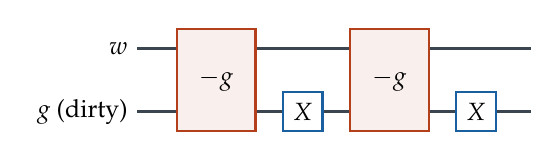
\begin{tikzpicture}[x=10mm,y=8mm]
        \node[lab] at (0,1) {$w$}; \node[lab] at (0,0) {$g$ (dirty)};
        \draw[wire] (0,1) -- (5,1); \draw[wire] (0,0) -- (5,0);
        \node[op,minimum width=10mm,minimum height=13mm] at (1,0.5) {$-g$};
        \node[hop] at (2.1,0) {$X$};
        \node[op,minimum width=10mm,minimum height=13mm] at (3.2,0.5) {$-g$};
        \node[hop] at (4.3,0) {$X$};
      \end{tikzpicture}\par
      \vskip2mm
      {\small $w-g-\overline g=w+1-2^{|w|}$\\for $g$ in \emph{any} state}
    \end{column}
    \begin{column}{0.48\textwidth}
      \small $g+\overline g$ is all ones, so two subtractions of a dirty register add 1 to $w$, and $g$ ends as it began (Gidney 2015).
      \vskip2mm
      No clean scratch: the qubits are borrowed from registers that are idle at that moment, whatever they hold.
    \end{column}
  \end{columns}
  \vskip2mm
  \code[basicstyle=\ttfamily\scriptsize]{inc_borrowed.py}
\end{frame}

\setcounter{framenumber}{186}
\begin{frame}{A controlled CDKM adder at $3n$ Toffolis, not $4n$}
  \begin{columns}[c]
    \begin{column}{0.44\textwidth}
      \centering
      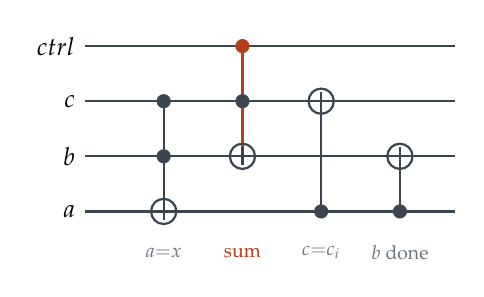
\begin{tikzpicture}[x=10mm,y=7mm]
        \foreach \y/\l in {3/ctrl,2/c,1/b,0/a} {\node[lab] at (0,\y) {$\l$}; \draw[wire] (0,\y) -- (4.7,\y);}
        \draw[thick,color=body] (1,2) -- (1,0); \node[dot] at (1,2) {}; \node[dot] at (1,1) {}; \oplusat{1}{0}
        \draw[thick,color=cverm] (2,3) -- (2,1); \node[dot,fill=cverm] at (2,3) {}; \node[dot] at (2,2) {}; \oplusat{2}{1}
        \draw[thick,color=body] (3,0) -- (3,2); \node[dot] at (3,0) {}; \oplusat{3}{2}
        \draw[thick,color=body] (4,0) -- (4,1); \node[dot] at (4,0) {}; \oplusat{4}{1}
        \node[note] at (1,-0.75) {$a{=}x$}; \node[note,color=cverm] at (2,-0.75) {sum};
        \node[note] at (3,-0.75) {$c{=}c_i$}; \node[note] at (4,-0.75) {$b$ done};
      \end{tikzpicture}\par
      \vskip1mm
      {\scriptsize the controlled UMA, after an \emph{uncontrolled} MAJ}
    \end{column}
    \begin{column}{0.52\textwidth}
      \small The package documented the textbook $3n$, but put the control on every MAJ and every UMA: $4n$.
      \vskip2mm
      Compute the carries \textbf{unconditionally} (one Toffoli a bit), and unwind them with a UMA that writes the sum bit only under the control (two). With the control off, $b$ returns to $y$.
      \vskip2mm
      {\color{cverm}\bfseries One of the lean cells corrected the package.}
    \end{column}
  \end{columns}
\end{frame}

\setcounter{framenumber}{187}
\begin{frame}[fragile]{The controlled CDKM adder, in code}
  \code[basicstyle=\ttfamily\scriptsize]{cdkm_cadd.py}
  \vskip2mm
  {\small On entry to \texttt{\_cuma}: $b=y\oplus x$, $c=c_i\oplus x$, $a=c_{i+1}$. The carries ripple up through plain MAJs and come down through controlled UMAs.}
\end{frame}

\setcounter{framenumber}{188}
\begin{frame}{Below 1\,000 qubits: share the lanes, vent a register}
  \begin{columns}[T]
    \begin{column}{0.47\textwidth}
      \blocktitle{Luo's extended Euclid}
      The remainders and cofactors share lanes, so the record disappears --- but each quotient bit costs a shifted comparison: $30\times$ the Toffolis for 139 qubits.
    \end{column}
    \begin{column}{0.47\textwidth}
      \blocktitle{Venting a register}
      Once $z=y/x$ exists, $y$ is a function of the others: it is $X$-measured and reused as the bank of the backward Euclid. The phase $(-1)^{b\cdot y}$ is cancelled by recomputing $y=xz$ around a $Z^b$.
    \end{column}
  \end{columns}
  \begin{takeaway}\texttt{ec\_mbu.vent} and \texttt{zfix}: the tests check that the phase cancels --- and that without the $Z^b$ it does not.\end{takeaway}
\end{frame}

\setcounter{framenumber}{189}
\begin{frame}{The register-shared Euclidean algorithm (Luo et al.)}
  \begin{columns}[c]
    \begin{column}{0.46\textwidth}
      \centering
      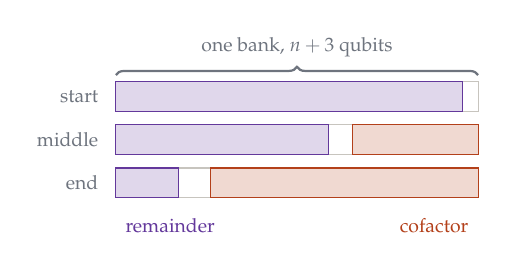
\begin{tikzpicture}[x=1mm,y=1mm]
        \foreach \y/\r/\c/\l in {11/44/0/start,5.5/27/16/{middle},0/8/34/end} {
          \draw[draw=rulegrey,fill=white] (0,\y) rectangle (46,\y+3.8);
          \draw[draw=cpurple,fill=cpurple!20] (0,\y) rectangle (\r,\y+3.8);
          \ifdim\c pt>0pt \draw[draw=cverm,fill=cverm!20] (46-\c,\y) rectangle (46,\y+3.8); \fi
          \node[font=\scriptsize,color=subtle,anchor=east] at (-1,\y+1.9) {\l};}
        \node[font=\scriptsize,color=cpurple,anchor=west] at (0,-3.5) {remainder};
        \node[font=\scriptsize,color=cverm,anchor=east] at (46,-3.5) {cofactor};
        \draw[decorate,decoration={brace,amplitude=3pt},thick,color=subtle] (0,15.6) -- (46,15.6) node[midway,above=3pt,font=\scriptsize] {one bank, $n+3$ qubits};
      \end{tikzpicture}
    \end{column}
    \begin{column}{0.5\textwidth}
      \small ECDSA.Fail's narrowest circuit drops the dialog: two remainders and two cofactors share two banks, the cofactors growing into the lanes the remainders free. \textbf{No record}.
      \vskip2mm
      The price: each quotient bit is a shifted comparison.
    \end{column}
  \end{columns}
  \vskip1.5mm
  \centering\footnotesize
  \renewcommand{\arraystretch}{1.05}
  \begin{tabular}{@{}rrrrrrr@{}}
    \toprule
    & \multicolumn{2}{c}{inversion} & \multicolumn{2}{c}{division} & \multicolumn{2}{c}{dialog division} \\
    \cmidrule(lr){2-3}\cmidrule(lr){4-5}\cmidrule(l){6-7}
    $n$ & qubits & Toffolis & qubits & Toffolis & qubits & Toffolis \\
    \midrule
    32 & 113 & 374\,232 & 177 & 779\,682 & 284 & 32\,686 \\
    64 & 183 & 1\,383\,179 & 311 & 2\,890\,248 & 546 & 120\,780 \\
    256 & \textbf{579} & 20\,433\,078 & \textbf{1\,091} & 42\,836\,318 & 2\,088 & \textbf{1\,749\,162} \\
    \bottomrule
  \end{tabular}\par
  \vskip1mm
  {\small Inversion: Luo's $2n+6\lfloor\log_2n\rfloor+19$ exactly. Division: half the dialog's qubits, $24\times$ its Toffolis.}
\end{frame}

\setcounter{framenumber}{190}
\begin{frame}{Three field registers, measured}
  \centering
  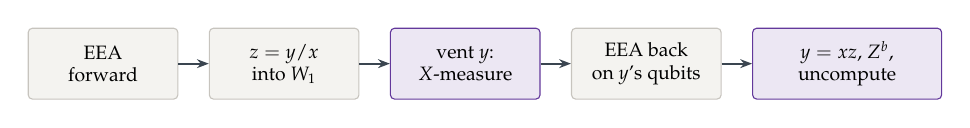
\begin{tikzpicture}[x=1mm,y=1mm,
      st/.style={draw=rulegrey,fill=greybox,rounded corners=1.5pt,minimum height=9mm,font=\scriptsize,align=center,inner sep=2pt},
      ar/.style={-{Stealth[length=1.5mm]},thick,color=body}]
    \node[st,minimum width=19mm] (a) at (0,0) {EEA\\forward};
    \node[st,minimum width=19mm] (b) at (23,0) {$z=y/x$\\into $W_1$};
    \node[st,minimum width=19mm,fill=cpurple!12,draw=cpurple] (c) at (46,0) {vent $y$:\\$X$-measure};
    \node[st,minimum width=19mm] (d) at (69,0) {EEA back\\on $y$'s qubits};
    \node[st,minimum width=24mm,fill=cpurple!12,draw=cpurple] (e) at (94.5,0) {$y=xz$, $Z^b$,\\uncompute};
    \foreach \u/\v in {a/b,b/c,c/d,d/e} \draw[ar] (\u) -- (\v);
  \end{tikzpicture}
  \vskip3mm
  \footnotesize
  \renewcommand{\arraystretch}{1.08}
  \begin{tabular}{@{}lrrr@{}}
    \toprule
    three field registers, secp256k1 & qubits & Toffolis & $X$-meas. \\
    \midrule
    in-place division (or multiplication) & \textbf{835} & 42\,103\,470 & 256 \\
    controlled addition of a classical point (Fig.~14) & 836 & 85\,039\,296 & 512 \\
    signed windowed addition, $w=16$ & \textbf{851} & 85\,204\,396 & 1\,792 \\
    whole ECDLP-256, 28 additions & 851 & 2\,385\,774\,798 & \\
    \midrule
    published: Luo et al.\ point addition & 835 & $70.29\times10^6$ & \\
    published: ECDSA.Fail, narrowest & 825--851 & & \\
    \bottomrule
  \end{tabular}\par
  \vskip2mm
  \raggedright{\small $3n+6\lfloor\log_2n\rfloor+19=835$ exactly, $+16$ window qubits. On Gidney's adder, exact for \emph{every} odd $p$: $835$ qubits, $44\,200\,815$ Toffolis.}
\end{frame}

\setcounter{framenumber}{191}
\begin{frame}[fragile]{Three field registers, in code}
  \code[basicstyle=\ttfamily\fontsize{7.3}{8.4}\selectfont]{div3.py}
  {\small Without the $Z^b$ the same circuit fails the phase check: the check can see what the vent does.}
\end{frame}

\setcounter{framenumber}{192}
\begin{frame}{7. Gidney's classical-quantum adder: $x\mathrel{+}=d$ on two clean qubits}
  \begin{columns}[T]
    \begin{column}{0.55\textwidth}
      The carries of $x+d$ are reproduced by adding $d$ into the complement of the result, so a streaming adder \emph{vents} each carry by $X$-measurement once its bit is summed.
      \vskip2mm
      The phases that leaves are undone on a \emph{dirty} register by $Z^m\cdot$carry-XOR$\cdot Z^m\cdot$carry-XOR.
      \vskip2mm
      {\small A vent cannot run backwards, so subtraction and halving are built forwards; on it the three-register circuits are exact for \emph{any} odd $p$.}
    \end{column}
    \begin{column}{0.41\textwidth}
      \begin{peachblock}\peachtitle{Measured, $n=256$}
        762 Toffolis ($2.98n$) on $n-1$ dirty $+$ 2 clean qubits.\par
        Luo's modular addition on it: 2\,813 ($10.99n$).
      \end{peachblock}
    \end{column}
  \end{columns}
\end{frame}

\setcounter{framenumber}{193}
\begin{frame}[fragile]{The vented adder, in code}
  \code[basicstyle=\ttfamily\scriptsize]{vented_add.py}
  {\small $c_{k+1}=\mathrm{maj}(x_k,d_k,c_k)$ costs one AND; $c_k$ is vented once $x_k$ is summed: two carry qubits suffice.}
\end{frame}

\setcounter{framenumber}{194}
\begin{frame}{The carry-XOR, derived rather than copied}
  \begin{columns}[T]
    \begin{column}{0.55\textwidth}
      \small The repair needs every carry XORed into a dirty $g$, since $Z_q\,CX_{c\to q}\,Z_q\,CX_{c\to q}=Z_c$. With $w_k=c_k\oplus x_k$ and $y_k=x_k\oplus d_k$:
      \[ w_{k+1}=(x_k\oplus x_{k+1})\oplus y_k\,w_k , \]
      one product per bit. Let $P$ be that pass on $g$, and $Q$ the same pass without the constants. Then $P(g)=w\oplus Q(g)$ with $Q$ linear and invertible, so
      \[ P\big(Q^{-1}(g)\big)=g\oplus w . \]
      Run $Q$ descending, then $P$, then XOR $x_k$ in to turn $w$ into $c$.
    \end{column}
    \begin{column}{0.41\textwidth}
      \begin{greyblock}[fontupper=\small]
        $\approx2n$ Toffolis, \textbf{no ancilla}. $d$ enters only through $X$ and CNOT gates, so a control on the constant costs nothing.
      \end{greyblock}
      \vskip1mm
      \centering\footnotesize
      \renewcommand{\arraystretch}{1.08}
      \begin{tabular}{@{}lrr@{}}
        \toprule
        $n=256$ & Toffolis & clean \\
        \midrule
        adder, $n-1$ dirty & 762 & 2 \\
        adder, no dirty & 1\,015 & 3 \\
        modular addition & 2\,813 & 5 \\
        modular doubling & 1\,535 & 4 \\
        \bottomrule
      \end{tabular}\par
      {\scriptsize $11.0n$ and $6.0n$: Luo et al.\ give $11n$ and $6n$}
    \end{column}
  \end{columns}
\end{frame}

\setcounter{framenumber}{195}
\begin{frame}[fragile]{The carry-XOR, in code}
  \code[basicstyle=\ttfamily\scriptsize]{carry_xor.py}
  \vskip1mm
  \begin{columns}[T]
    \begin{column}{0.48\textwidth}
      {\small The adder XORs each carry into $g$ as it goes: one carry-XOR then finishes the repair, $3n$ in all.}
    \end{column}
    \begin{column}{0.48\textwidth}
      {\small No dirty qubits: each half of the target serves the other, $4n$. A vent cannot be inverted.}
    \end{column}
  \end{columns}
\end{frame}

\setcounter{framenumber}{196}
\begin{frame}{8. Depth: carry-lookahead adders}
  \begin{columns}[c]
    \begin{column}{0.4\textwidth}
      \centering
      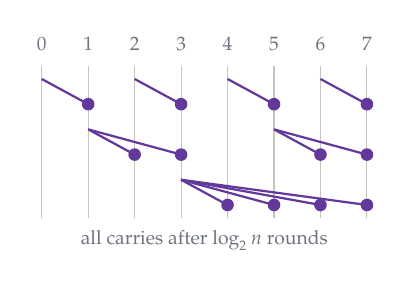
\begin{tikzpicture}[x=5.9mm,y=6.4mm]
        \foreach \i in {0,...,7} {\draw[color=rulegrey] (\i,3) -- (\i,0); \node[font=\scriptsize,color=subtle] at (\i,3.45) {\i};}
        \foreach \l/\s in {0/1,1/2,2/4} {
          \pgfmathtruncatemacro{\yy}{2-\l}
          \foreach \i in {0,...,7} {
            \pgfmathtruncatemacro{\b}{mod(floor(\i/\s),2)}
            \ifnum\b=1
              \pgfmathtruncatemacro{\j}{floor(\i/\s)*\s-1}
              \draw[thick,color=cpurple] (\j,\yy+0.75) -- (\i,\yy+0.25);
              \node[circle,fill=cpurple,inner sep=0pt,minimum size=1.6mm] at (\i,\yy+0.25) {};
            \fi}}
        \node[font=\scriptsize,color=subtle] at (3.5,-0.45) {all carries after $\log_2 n$ rounds};
      \end{tikzpicture}
    \end{column}
    \begin{column}{0.56\textwidth}
      \small On an error-corrected machine, time is Toffoli depth. Ripple adders, and the GCD's sequential rounds, make depth $0.8$--$0.95\times$ the Toffoli count.
      \vskip2mm
      [106] uses Draper--Kutin--Rains--Svore: carries as a prefix over (generate, propagate) pairs. The propagate rounds write clean ancillas: temporary ANDs, free to uncompute.
    \end{column}
  \end{columns}
  \vskip2mm
  \centering\footnotesize
  \renewcommand{\arraystretch}{1.05}
  \begin{tabular}{@{}rrrrrrr@{}}
    \toprule
    & \multicolumn{3}{c}{carry-lookahead} & \multicolumn{3}{c}{Gidney ripple} \\
    \cmidrule(lr){2-4}\cmidrule(l){5-7}
    $n$ & Toffolis & depth & qubits & Toffolis & depth & qubits \\
    \midrule
    8 & 27 & 11 & 25 & 7 & 7 & 23 \\
    64 & 395 & 23 & 243 & 63 & 63 & 191 \\
    256 & 1\,723 & \textbf{31} & 1\,007 & 255 & 255 & 767 \\
    \bottomrule
  \end{tabular}\par
  {\scriptsize depth $\approx4\log_2n$ for $\approx7n$ Toffolis}
\end{frame}

\setcounter{framenumber}{197}
\begin{frame}{Depth of one point addition: spend lookahead where the depth is}
  \centering\footnotesize
  \renewcommand{\arraystretch}{1.12}
  \begin{tabular}{@{}lrrr@{}}
    \toprule
    one windowed point addition, $n=256$, $w=16$ & qubits & Toffolis & Toffoli depth \\
    \midrule
    dialog, pseudo-Mersenne replay (ripple adders) & 2\,251 & 2\,000\,864 & 1\,503\,533 \\
    \quad $+$ carry-lookahead replay & 2\,601 & 6\,769\,556 & 936\,530 \\
    \quad $+$ carry-lookahead walk & 2\,601 & 8\,655\,996 & 456\,379 \\
    \quad $+$ carry-lookahead squarer & 2\,601 & 9\,184\,472 & 394\,281 \\
    \quad $+$ register sharing, Fig.~1 packing & 2\,223 & 9\,189\,792 & \textbf{394\,917} \\
    \bottomrule
  \end{tabular}\par
  \vskip3mm
  \raggedright
  \begin{columns}[T]
    \begin{column}{0.48\textwidth}
      \small \textbf{Fan out the controls.} $n$ Toffolis sharing one control take $n$ steps: a qubit is in one gate at a time. Copy the control to $n$ qubits with CNOTs first --- no Toffoli depth.
    \end{column}
    \begin{column}{0.48\textwidth}
      \small \textbf{Measured, not estimated.} \texttt{hier.exact\_depth} schedules the cached hierarchy gate by gate without building the flat circuit; at toy size it equals the flat depth.
    \end{column}
  \end{columns}
  \begin{takeaway}Depth $\div3.8$ for $4.6\times$ the Toffolis --- at the same width, once the record is shared.\end{takeaway}
\end{frame}

\setcounter{framenumber}{198}
\begin{frame}{The depth frontier, and the floor the lookups set}
  \begin{columns}[c]
    \begin{column}{0.62\textwidth}
      \centering
      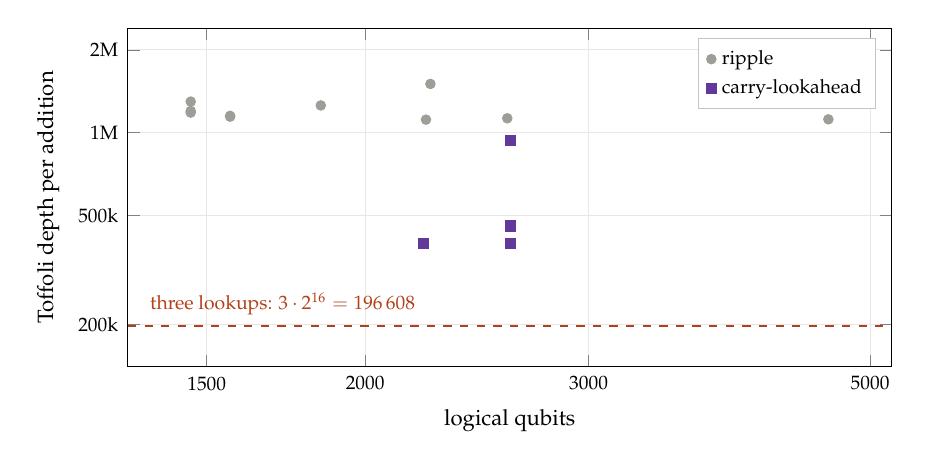
\begin{tikzpicture}
      \begin{axis}[scale only axis,width=0.8\linewidth,height=4.3cm,xmode=log,ymode=log,xmin=1300,xmax=5200,ymin=1.4e5,ymax=2.4e6,
        ytick={2e5,5e5,1e6,2e6},yticklabels={200k,500k,1M,2M},
        xlabel={logical qubits},ylabel={Toffoli depth per addition},xtick={1500,2000,3000,5000},xticklabels={1500,2000,3000,5000},
        grid=both,clip mode=individual,legend style={at={(0.98,0.97)},anchor=north east,font=\scriptsize}]
        \addplot[only marks,mark=*,mark size=1.7pt,rulegrey!80!black] coordinates {
          (2251,1503533) (2233,1114102) (1845,1255253) (1457,1296204) (1457,1198152) (1457,1182024)
          (1565,1150276) (1565,1142347) (2588,1126989) (4635,1117009)};\addlegendentry{ripple}
        \addplot[only marks,mark=square*,mark size=1.8pt,cpurple] coordinates {
          (2601,936530) (2601,456379) (2601,394281) (2223,394917)};\addlegendentry{carry-lookahead}
        \draw[cverm,thick,dashed] (axis cs:1300,196608) -- (axis cs:5200,196608);
        \node[font=\scriptsize,cverm,anchor=south west] at (axis cs:1330,200000) {three lookups: $3\cdot2^{16}=196\,608$};
      \end{axis}
      \end{tikzpicture}
    \end{column}
    \begin{column}{0.35\textwidth}
      \small Unary iteration over $2^{16}$ entries is $2^{16}$ steps deep, so no arithmetic gets below the floor.
      \vskip2mm
      \textbf{Reusing a qubit orders the steps that use it.} The $1\,457$-qubit circuit is $33.6$M deep in all; the $2\,233$-qubit one, $29.5$M.
    \end{column}
  \end{columns}
\end{frame}

\setcounter{framenumber}{199}
\begin{frame}{9. Catalogue: a looked-up addend in Jacobian coordinates}
  \begin{columns}[T]
    \begin{column}{0.54\textwidth}
      \centering\footnotesize
      \renewcommand{\arraystretch}{1.1}
      \begin{tabular}{@{}lrr@{}}
        \toprule
        one addition, $n=32$ & qubits & Toffolis \\
        \midrule
        affine, in place, controlled & 540 & 262\,797 \\
        Jacobian $+$ classical affine & 742 & 157\,680 \\
        Jacobian $+$ quantum affine & 806 & 174\,900 \\
        \quad controlled & 903 & 175\,250 \\
        Jacobian $+$ quantum Jacobian & 998 & 257\,460 \\
        \quad controlled & 1\,095 & 257\,810 \\
        \midrule
        to affine, once per run & 571 & 139\,066 \\
        \bottomrule
      \end{tabular}
    \end{column}
    \begin{column}{0.42\textwidth}
      \small [106] Alg.~4 with the addend looked up rather than classical (\texttt{ec\_proj\_q}).
      \vskip2mm
      \textbf{A cheaper addition is not a cheaper oracle.} A projective triple depends on the path that made it, so the chain must be undone before anything is read.
    \end{column}
  \end{columns}
  \vskip3mm
  \centering
  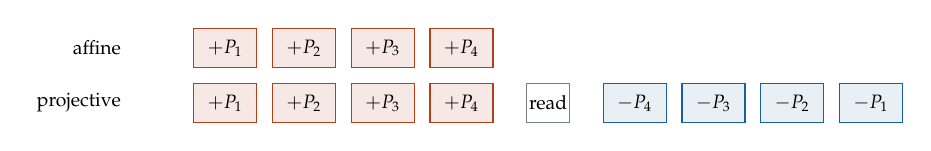
\begin{tikzpicture}[x=1mm,y=1mm,ad/.style={draw=cverm,fill=cverm!12,minimum width=8mm,minimum height=5mm,font=\scriptsize,inner sep=1pt},un/.style={draw=cblue,fill=cblue!10,minimum width=8mm,minimum height=5mm,font=\scriptsize,inner sep=1pt}]
    \node[font=\scriptsize,anchor=east] at (-2,7) {affine};
    \foreach \i in {1,...,4} \node[ad] at (\i*10,7) {$+P_\i$};
    \node[font=\scriptsize,anchor=east] at (-2,0) {projective};
    \foreach \i in {1,...,4} \node[ad] at (\i*10,0) {$+P_\i$};
    \node[meter] at (51,0) {read};
    \foreach \i in {4,...,1} \node[un] at (102-\i*10,0) {$-P_\i$};
  \end{tikzpicture}\par
  {\scriptsize Undoing doubles the additions: at toy size the projective oracle costs about twice the affine one.}
\end{frame}

\setcounter{framenumber}{200}
\begin{frame}{Catalogue: twisted Edwards curves}
  \begin{columns}[c]
    \begin{column}{0.5\textwidth}
      \small Extended twisted Edwards coordinates ([106] Sec.~4.4, \texttt{ec\_edwards}) have a \textbf{complete} addition law: no exceptional cases at all.
      \vskip2mm
      7 multiplications where Jacobian needs 11.
    \end{column}
    \begin{column}{0.46\textwidth}
      \begin{peachblock}[fontupper=\small]\peachtitle{With a classical addend}
        $3.2\times$ fewer Toffolis and $26\%$ fewer qubits than Weierstrass Jacobian, at both sizes.
      \end{peachblock}
    \end{column}
  \end{columns}
  \vskip4mm
  \centering\footnotesize
  \renewcommand{\arraystretch}{1.15}
  \begin{tabular}{@{}rrrrr@{}}
    \toprule
    & \multicolumn{2}{c}{Edwards (Ed25519-shaped)} & \multicolumn{2}{c}{Weierstrass Jacobian} \\
    \cmidrule(lr){2-3}\cmidrule(l){4-5}
    $n$ & Toffolis & qubits & Toffolis & qubits \\
    \midrule
    32 & \textbf{44\,438} & 550 & 143\,796 & 742 \\
    64 & \textbf{172\,090} & 1\,094 & 566\,132 & 1\,478 \\
    \bottomrule
  \end{tabular}\par
  \vskip2mm
  {\scriptsize secp256k1 is not an Edwards curve: this is a catalogue entry, not a step of the ECDLP-256 circuit.}
\end{frame}

\setcounter{framenumber}{201}
\begin{frame}{Catalogue: batch inversion}
  \begin{columns}[c]
    \begin{column}{0.5\textwidth}
      \centering
      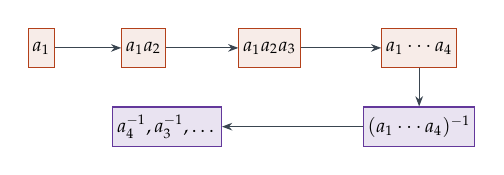
\begin{tikzpicture}[x=1mm,y=1mm,
          bx/.style={draw=cverm,fill=cverm!10,minimum height=5mm,font=\scriptsize,inner sep=1.5pt},
          iv/.style={draw=cpurple,fill=cpurple!14,minimum height=5mm,font=\scriptsize,inner sep=1.5pt},
          ar/.style={-{Stealth[length=1.3mm]},color=body}]
        \node[bx] (p1) at (0,10) {$a_1$};
        \node[bx] (p2) at (13,10) {$a_1a_2$};
        \node[bx] (p3) at (29,10) {$a_1a_2a_3$};
        \node[bx] (p4) at (48,10) {$a_1\cdots a_4$};
        \foreach \u/\v in {p1/p2,p2/p3,p3/p4} \draw[ar] (\u) -- (\v);
        \node[iv] (inv) at (48,0) {$(a_1\cdots a_4)^{-1}$};
        \draw[ar] (p4) -- (inv);
        \node[iv] (o) at (16,0) {$a_4^{-1},a_3^{-1},\dots$};
        \draw[ar] (inv) -- (o);
      \end{tikzpicture}\par
      {\scriptsize one inversion, $3(k-1)$ multiplications}
    \end{column}
    \begin{column}{0.46\textwidth}
      \small Litinski shares one inversion across $k$ independent affine additions. Built \emph{clean}, every intermediate uncomputed: 2 inversions $+\,5(k-1)$ multiplications, against $2k$ inversions.
    \end{column}
  \end{columns}
  \vskip2mm
  \centering\footnotesize
  \renewcommand{\arraystretch}{1.05}
  \begin{tabular}{@{}rrlrrrr@{}}
    \toprule
    & & & \multicolumn{2}{c}{Toffolis} & \multicolumn{2}{c}{qubits} \\
    \cmidrule(lr){4-5}\cmidrule(l){6-7}
    $n$ & $k$ & what & separate & batched & separate & batched \\
    \midrule
    64 & 2 & inversions & 703\,732 & 516\,346 & 1\,054 & 1\,118 \\
    64 & 8 & inversions & 2\,814\,928 & \textbf{1\,503\,226} & 1\,822 & 2\,510 \\
    256 & 4 & inversions & 22\,169\,576 & 13\,414\,394 & 5\,156 & 5\,924 \\
    256 & 4 & point additions & 65\,369\,012 & 46\,815\,704 & 5\,672 & 7\,445 \\
    \bottomrule
  \end{tabular}\par
  \vskip1mm
  \raggedright{\small Always fewer Toffolis, always more qubits --- and only on the Kaliski path: in the dialog a multiplication costs as much as an inversion.}
\end{frame}

\setcounter{framenumber}{202}
\begin{frame}[fragile]{Catalogue: ECDSA.Fail's fire census}
  \begin{columns}[T]
    \begin{column}{0.54\textwidth}
      \code[basicstyle=\ttfamily\scriptsize]{census.py}
    \end{column}
    \begin{column}{0.42\textwidth}
      \centering\footnotesize
      \renewcommand{\arraystretch}{1.1}
      \begin{tabular}{@{}rrr@{}}
        \toprule
        sample & Toffolis left & wrong \\
        \midrule
        10 & 752 & 98.0\% \\
        30 & 891 & 65.2\% \\
        100 & 957 & 10.2\% \\
        300 & 984 & 2.8\% \\
        every input & 991 & 0 \\
        \bottomrule
      \end{tabular}\par
      {\scriptsize the $q=61$ dialog multiplier (1\,680 Toffolis); wrong: share of fresh inputs}
    \end{column}
  \end{columns}
  \vskip3mm
  \begin{columns}[T]
    \begin{column}{0.48\textwidth}
      \small Run a sample, record which Toffolis ever fired, delete the rest. Over \emph{every} input it is exact dead-code removal; over a sample it is a guess.
    \end{column}
    \begin{column}{0.48\textwidth}
      \small The dead code is the round budget's padding. At $n=256$ that is the $2.4\sqrt n$ margin rounds: a census finds only what they never did \emph{on the inputs it saw}.
    \end{column}
  \end{columns}
\end{frame}

\setcounter{framenumber}{203}
\begin{frame}{10. RSA at size: Gidney 2025's residue arithmetic, loop for loop}
  Per prime of the residue system: look up and add the dlogs of the window multipliers, reduce mod $p-1$, exponentiate by windowed multiplications (old results measured out), subtract the truncated CRT term into an $f$-bit accumulator.
  \vskip2mm
  \centering\small
  \renewcommand{\arraystretch}{1.15}
  \begin{tabular}{@{}rrrrr@{}}
    \toprule
    $n$ & primes & Toffolis, built & Gidney 2025 & qubits, built (paper) \\
    \midrule
    1024 & 6\,242 & $1.18\times10^9$ & $1.1\times10^9$ & 800 (742) \\
    2048 & 21\,320 & $\mathbf{6.95\times10^9}$ & $6.5\times10^9$ & 1\,467 (1\,399) \\
    3072 & 47\,814 & $1.97\times10^{10}$ & $1.9\times10^{10}$ & 2\,115 (2\,043) \\
    4096 & 74\,245 & $4.29\times10^{10}$ & $4\times10^{10}$ & 2\,766 (2\,692) \\
    \bottomrule
  \end{tabular}
  \vskip2mm
  \raggedright{\small At toy $N$ the circuit equals a bit-exact model on every exponent; at size one prime's iteration is built and multiplied by the number of primes.}
\end{frame}

\setcounter{framenumber}{204}
\begin{frame}{ECDLP against RSA, on one surface-code model}
  \centering\small
  \renewcommand{\arraystretch}{1.15}
  \begin{tabular}{@{}lrrrr@{}}
    \toprule
    whole algorithm (built) & logical qubits & Toffolis & physical qubits & time \\
    \midrule
    ECDLP-256, IonQ cells, signed windows & 1\,457 & $3.7\times10^7$ & 2.14M & 15 min \\
    ECDLP-256, dialog, space cells & 1\,246 & $7.9\times10^7$ & 1.85M & 33 min \\
    ECDLP-256, three registers & 851 & $2.4\times10^9$ & 1.32M & 0.73 d \\
    RSA-2048, Gidney 2025 & 1\,467 & $7.0\times10^9$ & 0.97M & 2.1 d \\
    RSA-3072, Gidney 2025 & 2\,115 & $2.0\times10^{10}$ & 1.26M & 6.4 d \\
    \bottomrule
  \end{tabular}
  \vskip2mm
  \raggedright{\small One model for every row: $p=10^{-3}$, $1\,\mu$s cycle, $10\,\mu$s reaction, six CCZ factories. It reproduces Gidney's 897\,864 qubits / 4.96 days.}
  \begin{takeaway}At comparable width, secp256k1 costs $189\times$ fewer Toffolis than RSA-2048 and $537\times$ fewer than RSA-3072, its classical-security equal.\end{takeaway}
\end{frame}

\setcounter{framenumber}{208}
\begin{frame}{Act XII in plain words (3/3)}
  \centering\footnotesize
  \renewcommand{\arraystretch}{1.15}
  \begin{tabular}{@{}>{\raggedright}p{30mm}>{\raggedright}p{63mm}>{\raggedright\arraybackslash\leavevmode\color{cverm}}p{40mm}@{}}
    \toprule
    optimisation & what it does & \color{ink}what it bought \\
    \midrule
    \textbf{Luo's register-shared Euclid} & remainders and cofactors share qubit banks, so no record is kept & $1\,246\to1\,107$ qubits for $30\times$ the Toffolis \\
    \textbf{Three registers, venting $y$} & measure $y$ away once it can be recomputed; repair the phase with $Z$ around $y=xz$ & 851 qubits, $85.2$M Toffolis per addition \\
    \textbf{Gidney's adder, carry-XOR} & add a constant on 2 clean and borrowed dirty qubits; vented carries repaired by a derived carry-XOR & 762 Toffolis; exact for any odd $p$ \\
    \textbf{Carry-lookahead, fan-out} & log-depth carries; each shared control copied onto $n$ qubits first & depth $1.50\to0.39$M, $4.6\times$ the Toffolis \\
    \bottomrule
  \end{tabular}
  \par\vskip1mm{\scriptsize\color{subtle}The catalogue entries (looked-up addend, Edwards curves, batch inversion, fire census) are built and measured but not in the headline circuit.}
\end{frame}

% ======================================================================
\appendix
\setbeamertemplate{footline}{\hfill{\scriptsize\color{ink}B\insertframenumber}\hspace*{5mm}\vskip3mm}
\begin{frame}{Backup --- why the QFT ends with swaps}
  Output qubit $q$ needs the phase $e^{2\pi i\,j2^q/2^n}$, which depends only on the lowest $n-q$ bits of $j$. The in-place loop builds that factor on qubit $n-1-q$.
  \vskip2mm
  \centering\small
  \begin{tabular}{lccc}
    \toprule
    phase on each qubit ($\times2\pi$), input $|1\rangle$, $n=3$ & qubit 0 & qubit 1 & qubit 2 \\
    \midrule
    required: $j2^q/2^n$ & 0.125 & 0.250 & 0.500 \\
    the loop without the swaps & 0.500 & 0.250 & 0.125 \\
    \texttt{qft()}, with the swaps & 0.125 & 0.250 & 0.500 \\
    \bottomrule
  \end{tabular}
  \vskip2mm
  \raggedright
  \begin{takeaway}The swaps are bookkeeping (3 CNOT, 0 T): before a measurement, inside an adder, or in the semiclassical QFT the reversal is absorbed by relabelling.\end{takeaway}
\end{frame}

\begin{frame}{Backup --- measured counts against the formulas}
  \begin{columns}[c]
  \begin{column}{0.62\textwidth}
  \centering\footnotesize
  \setlength{\tabcolsep}{3pt}
  \begin{tabular}{@{}rrrrrrrr@{}}
    \toprule
    $n$ & $N$ & qubits & $4n+2$ & Toffoli & $8n^3+22n^2$ & CP & formula \\
    \midrule
    4 & 15 & 18 & 18 & 864 & 864 & 7\,068 & 7\,068 \\
    5 & 21 & 22 & 22 & 1\,550 & 1\,550 & 16\,245 & 16\,245 \\
    6 & 33 & 26 & 26 & 2\,520 & 2\,520 & 32\,322 & 32\,322 \\
    7 & 65 & 30 & 30 & 3\,822 & 3\,822 & 58\,107 & 58\,107 \\
    8 & 129 & 34 & 34 & 5\,504 & 5\,504 & 96\,888 & 96\,888 \\
    \bottomrule
  \end{tabular}
  \end{column}
  \begin{column}{0.36\textwidth}
  \centering\fig[width=\textwidth]{factoring_scaling.pdf}
  \end{column}
  \end{columns}
\end{frame}

\begin{frame}[fragile]{Backup --- counting in code}
  \begin{columns}[T]
    \begin{column}{0.56\textwidth}
      \code[basicstyle=\ttfamily\footnotesize]{resources.py}
      {\small prints \texttt{18 864 7068 12855} and \texttt{14309 978434}.}
    \end{column}
    \begin{column}{0.4\textwidth}
      \scriptsize
      \renewcommand{\arraystretch}{1.1}
      \begin{tabular}{ll}
        \toprule
        gate & priced as \\
        \midrule
        CCX, CSWAP & 1 Toffoli, 7 T \\
        MCX, $k$ controls & $2k-3$ Toffolis \\
        MCP, $k$ controls & $2(k-1)$ Toffolis + CP \\
        $\mathrm{CP}(\theta)$ & 2 CNOT + 3 $P(\pm\theta/2)$ \\
        $P(\theta)$, $\theta\notin\frac\pi4\mathbb{Z}$ & 1 small rotation \\
        temporary AND & 4 T, uncompute 0 \\
        \bottomrule
      \end{tabular}
    \end{column}
  \end{columns}
\end{frame}

\begin{frame}[fragile]{Backup --- Draper's adder in Qiskit}
  \code[basicstyle=\ttfamily\scriptsize]{add_const.py}
\end{frame}

\begin{frame}[fragile]{Backup --- the modular adder in Qiskit}
  \code[basicstyle=\ttfamily\scriptsize]{c_add_mod.py}
\end{frame}

\begin{frame}[fragile]{Backup --- the ripple-carry adder in Qiskit}
  \code[basicstyle=\ttfamily\footnotesize]{rc_add.py}
  \vskip2mm
  {\small \texttt{ctrls} reach only the two CNOTs into $b$ of each MAJ and UMA (\texttt{rc\_majuma.py}, Act VII).}
\end{frame}

\begin{frame}[fragile]{Backup --- the ripple-carry modular adder: control on two blocks}
  \code[basicstyle=\ttfamily\fontsize{7.2}{8.3}\selectfont]{rc_c_add_mod.py}
\end{frame}

\begin{frame}[fragile]{Backup --- factoring end to end, retrying}
  \code[basicstyle=\ttfamily\footnotesize]{find_factor.py}
  \vskip2mm
  \texttt{run}: any circuit $\to$ counts.
\end{frame}

\begin{frame}[fragile]{Backup --- the garbage demo is one extra line}
  \code[basicstyle=\ttfamily\footnotesize]{garbage.py}
\end{frame}

\begin{frame}[fragile]{Backup --- ECDLP: votes for $k$}
  \code[basicstyle=\ttfamily\footnotesize]{ecdlp_post.py}
\end{frame}

\begin{frame}[fragile]{Backup --- ECDLP end to end}
  \code[basicstyle=\ttfamily\footnotesize]{ecdlp_run.py}
\end{frame}

\begin{frame}{Backup --- how the circuits are verified}
  \begin{columns}[T]
    \begin{column}{0.31\textwidth}
      \begin{greyblock}[fontupper=\small]
        \blocktitle{Arithmetic, exactly}
        Every block on every basis input; every ancilla checked back to $|0\rangle$ where it is freed.
      \end{greyblock}
    \end{column}
    \begin{column}{0.31\textwidth}
      \begin{greyblock}[fontupper=\small]
        \blocktitle{Distributions, exactly}
        Closed-form $P(y)$ against Aer's exact probabilities: equal to $10^{-14}$.
      \end{greyblock}
    \end{column}
    \begin{column}{0.31\textwidth}
      \begin{greyblock}[fontupper=\small]
        \blocktitle{Samples, statistically}
        Every histogram within the distance a perfect sampler reaches at that shot count.
      \end{greyblock}
    \end{column}
  \end{columns}
  \vskip3mm
  \begin{takeaway}Test the distribution, not the factors: a broken circuit gives a flat histogram, and the classical checks can still print the right factors by luck.\end{takeaway}
\end{frame}

\begin{frame}{Backup --- elliptic curves against RSA, across key sizes}
  \centering\small
  \begin{tabular}{rrr@{\hspace{10mm}}rrr}
    \toprule
    ECC bits & qubits & Toffoli & RSA bits & qubits & Toffoli \\
    \midrule
    160 & 1\,466 & $3.0\times10^{10}$ & 1\,024 & 2\,050 & $5.8\times10^{11}$ \\
    224 & 2\,042 & $8.4\times10^{10}$ & 2\,048 & 4\,098 & $5.2\times10^{12}$ \\
    256 & 2\,330 & $1.3\times10^{11}$ & 3\,072 & 6\,146 & $1.9\times10^{13}$ \\
    384 & 3\,484 & $4.5\times10^{11}$ & 7\,680 & 15\,362 & $3.3\times10^{14}$ \\
    521 & 4\,719 & $1.1\times10^{12}$ & 15\,360 & 30\,722 & $2.9\times10^{15}$ \\
    \bottomrule
  \end{tabular}
  \vskip3mm
  \raggedright{\small Rows pair comparable classical security. Minimal-width logical counts: Roetteler--Naehrig--Svore--Lauter (2017; $9n+2\lceil\log_2 n\rceil+10$ qubits, $(448\log_2 n+4090)\,n^3$ Toffolis) and Häner--Roetteler--Svore (2017; $2n+2$ qubits). Error correction multiplies both sides by comparable factors.}
\end{frame}

\begin{frame}[fragile]{Backup --- reproduce every number}
\begin{lstlisting}[language=bash,basicstyle=\ttfamily\small,morekeywords={}]
python3 -m venv venv && venv/bin/pip install -r requirements.txt
./run_tests.sh fast      # incl. semiclassical QFT and resource counts
./run_tests.sh full      # + end-to-end factoring on Aer
./run_tests.sh ec        # the ECDLP suite
venv/bin/jupyter lab notebooks/shor_walkthrough.ipynb
venv/bin/python presentation/make_figures.py    # this deck's figures
venv/bin/python presentation/make_listings.py   # its code, checked
\end{lstlisting}
\end{frame}

\begin{frame}{Backup --- references, Acts I--IX}
  \footnotesize
  \begin{itemize}\setlength{\itemsep}{1.2mm}
    \item P. W. Shor, SIAM J. Comput. 26 (1997). \quad S. Beauregard, Quantum Inf. Comput. 3 (2003).
    \item T. G. Draper, quant-ph/0008033. \quad S. Cuccaro, T. Draper, S. Kutin, D. Moulton, quant-ph/0410184.
    \item R. Griffiths, C.-S. Niu, Phys. Rev. Lett. 76 (1996). \quad C. H. Bennett, IBM J. Res. Dev. 17 (1973). \quad T. Toffoli, ICALP 1980.
    \item C. Dawson, M. Nielsen, quant-ph/0505030. \quad N. J. Ross, P. Selinger, arXiv:1403.2975.
    \item C. Gidney, arXiv:1709.06648 (temporary AND); arXiv:1905.07682 (windowing); arXiv:2505.15917 (2025).
    \item C. Gidney, M. Ekerå, Quantum 5, 433 (2021). \quad D. Litinski, arXiv:2306.08585 (2023).
    \item M. Roetteler, M. Naehrig, K. Svore, K. Lauter, ASIACRYPT 2017. \quad T. Häner, M. Roetteler, K. Svore, arXiv:1611.07995.
    \item Kim et al., eprint 2026/106. \quad A. Schrottenloher, eprint 2026/1128. \quad NIST SP 800-57; FIPS 203, 204.
  \end{itemize}
\end{frame}

\begin{frame}{Backup --- references, the optimisations (Acts VII, VIII, XII)}
  \footnotesize
  \begin{itemize}\setlength{\itemsep}{1.1mm}
    \item \textbf{Factoring.} C. Zalka, quant-ph/9806084; quant-ph/0601097 (coset representation). \ C. Gidney, M. Ekerå, Quantum 5, 433 (2021). \ R. Griffiths, C.-S. Niu, quant-ph/9511007. \ A. Barenco et al., quant-ph/9601018.
    \item S. Cuccaro, T. Draper, S. Kutin, D. Moulton, quant-ph/0410184. \ C. Gidney, Quantum 2, 74 (2018) (temporary AND); arXiv:1905.07682 (windows). \ R. Babbush et al., Phys. Rev. X 8, 041015 (2018) (unary iteration).
    \item \textbf{ECDLP.} H. Kim et al., eprint 2026/106. \ A. Schrottenloher, eprint 2026/1128. \ T. Häner, S. Jaques, M. Naehrig, M. Roetteler, M. Soeken, PQCrypto 2020. \ T. Khattar et al., arXiv:2510.10967. \ M. Grassl et al., PQCrypto 2016 (zig-zag).
    \item \textbf{Act XII.} IonQ, arXiv:2609.05625. \ ECDSA.Fail, arXiv:2609.09582. \ H. Luo et al., arXiv:2607.13816. \ D. Litinski, arXiv:2306.08585. \ G. H. Low, V. Kliuchnikov, L. Schaeffer, arXiv:1812.00954.
    \item T. Draper, S. Kutin, E. Rains, K. Svore, quant-ph/0406142 (carry-lookahead). \ C. Gidney, \emph{Constructing large increment gates} (2015); arXiv:2507.23079. \ T. Häner, M. Roetteler, K. Svore, arXiv:1611.07995.
  \end{itemize}
\end{frame}

\begin{frame}{Backup --- references, Act X (Hamiltonians and hardware)}
  \footnotesize
  \begin{itemize}\setlength{\itemsep}{1.2mm}
    \item R. W. Brockett, SIAM J. Control 10 (1972). \ V. Jurdjevic, H. Sussmann, J. Diff. Eq. 12 (1972). \ D. D'Alessandro, \emph{Quantum Control and Dynamics} (2021).
    \item N. Khaneja, S. Glaser, quant-ph/0010100. \ B. Kraus, J. I. Cirac, quant-ph/0011050. \ J. Zhang et al., quant-ph/0209120 (Weyl chamber). \ R. Wiersema et al., npj QI 10, 110 (2024).
    \item J. Koch et al., cond-mat/0703002 (transmon). \ F. Motzoi et al., 0901.0534 (DRAG). \ E. Magesan, J. Gambetta, 1804.04073 (cross-resonance). \ Google, Willow spec sheet (2024).
    \item A. S{\o}rensen, K. M{\o}lmer, quant-ph/9810039. \ A. C. Hughes et al., arXiv:2510.17286 (99.99\%). \ A. Ransford et al., Nature 655, 81 (2026) (Helios).
    \item D. Jaksch et al., quant-ph/0004038. \ H. Levine et al., 1908.06101. \ S. Jandura, G. Pupillo, 2202.00903. \ S. Evered et al., Nature 622, 268 (2023); arXiv:2604.25987.
    \item D. Loss, D. DiVincenzo, cond-mat/9701055. \ P. Steinacker et al., Nature 646, 81 (2025). \ E. Knill, R. Laflamme, G. Milburn, quant-ph/0006088. \ PsiQuantum, Nature 641, 876 (2025).
    \item S. Puri et al., 1605.09408 (Kerr cat). \ H. Putterman et al., Nature 638, 927 (2025). \ Y. Wu et al., 2201.03540 (erasure). \ Tutorial \S9--\S10 and Appendix C: derivations and numerical checks.
  \end{itemize}
\end{frame}

\begin{frame}{Backup --- references, Acts XI--XII}
  \footnotesize
  \begin{itemize}\setlength{\itemsep}{1.2mm}
    \item \textbf{Act XI.} Babbush et al., arXiv:2603.28846. \ Schrottenloher, arXiv:2606.02235. \ Luo et al., arXiv:2607.13816. \ ECDSA.Fail, arXiv:2609.09582. \ IonQ, arXiv:2609.05625.
    \item Webster et al., arXiv:2602.11457 (Pinnacle). \ Cain et al., arXiv:2603.28627 (Oratomic). \ Bravyi et al., Nature 627 (2024). \ Gidney, Shutty, Jones, arXiv:2409.17595. \ Müller et al., arXiv:2506.01779.
    \item \textbf{Act XII.} Gidney, arXiv:2507.23079. \ Low, Kliuchnikov, Schaeffer, arXiv:1812.00954. \ \texttt{shor-complete.tex} Parts VII--VIII; \texttt{bench/}.
  \end{itemize}
\end{frame}

\end{document}
